%%%%%%%%%%%%%%%%%%%%%%%%%%%%%%%%%%%%%%%%%%%%%%%%%%%%%%%
%
%                                                       Example IS Template
%
% \documentclass{woosterthesis} must be at the beginning of every IS. Options are the same as
% for the report class with some additional options: abstractonly, acs, alltt, apa, blacklinks, chicago,
% code, colophon, dropcaps, euler, foreignlanguage, gauss, index, kaukecopyright, lshortwooster, maple, mla, palatino, picins,tikz,
% verbatim, wblack, and woostercopyright. The kaukecopyright option will put the arch symbol with the word mark on the
% copyright page. The woosterthesis class is based on the report class. One thing to note is that
% the ``%'' symbol comments out all characters that follow it on the line.
%
%%%%%%%%%%%%%%%%%%%%%%%%%%%%%%%%%%%%%%%%%%%%%%%%%%%%%%%

%%%%%%%%%%%%%%%%%%%%%%%%%%%%%%%%%%%%%%%%%%%%%%%%%%%%%%%
%
% Checked on 8/26/22 and compiles with no fatal errors. Users must have the latest version of the TeXLive software and
% have installed all available packages from CTAN to ensure this thesis class compiles with no fatal errors. Also, you must
% run pdfLaTex, Biber, MakeIndex, padfLaTeX, pdfLaTeX to get all the numbering and references resolved. This is the
% first year the template uses Biber for references.
%
%%%%%%%%%%%%%%%%%%%%%%%%%%%%%%%%%%%%%%%%%%%%%%%%%%%%%%%

%%%%%%%%%%%%%%%%%%%%%%%%%%%%%%%%%%%%%%%%%%%%%%%%%%%%%%%
% use this declaration for a draft  version of your IS
\documentclass[10pt,palatino,code,picins,tikz,kaukecopyright,openright,lshortwooster,dropcaps,verbatim,index,euler]{woosterthesis}
% Note that you can specify the acs option to use the American Chemical Society citation format, apa option to use the American
% Psychological Association citation format, chicago option to use the Chicago citation format, mla option to use the Modern Language
% Association citation format, wblack option for a grayscale Wooster "W" on the cover, and scottie option for a grayscale Scottie Mascot
% on the cover. See exampleis_manual.pdf for an explanation of all the options.
%
%%%%%%%%%%%%%%%%%%%%%%%%%%%%%%%%%%%%%%%%%%%%%%%%%%%%%%%
%
% use this declaration for the print version of your IS
%\documentclass[12pt,code,palatino,picins,blacklinks,kaukecopyright,openright]{woosterthesis} % probably what most students would use
%
%%%%%%%%%%%%%%%%%%%%%%%%%%%%%%%%%%%%%%%%%%%%%%%%%%%%%%%
%
% use this declaration for the PDF version of your IS
%\documentclass[12pt,code,palatino,picins,kaukecopyright,openright]{woosterthesis}
%
%%%%%%%%%%%%%%%%%%%%%%%%%%%%%%%%%%%%%%%%%%%%%%%%%%%%%%%

%%%%%%%%%%%%%%%%%%%%%%%%%%%%%%%%%%%%%%%%%%%%%%%%%%%%%%%
%
%                                                       Load Packages
%
%   To load packages in addition to the ones that are loaded by default, please place your
%   usepackage commands in the packages.tex file in the styles folder.
%
%%%%%%%%%%%%%%%%%%%%%%%%%%%%%%%%%%%%%%%%%%%%%%%%%%%%%%%

%%%%%%%%%%%%%%%%%%%%%%%%%%%%%%%%%%%%%%%%%%%%%%%%%%%%%%%%%%%%%%%%%%%%%%%%%%%%%%%%%%%%%%%%%%%%%%
%
%                                                       Packages
%
% Do not add any other packages without consulting with Dr. Breitenbucher as they may break the functionality of the class.
%
%%%%%%%%%%%%%%%%%%%%%%%%%%%%%%%%%%%%%%%%%%%%%%%%%%%%%%%%%%%%%%%%%%%%%%%%%%%%%%%%%%%%%%%%%%%%%%

\ifxetex%
	\defaultfontfeatures{Mapping=tex-text,Ligatures=TeX}%
		\setmainfont[Numbers=OldStyle,BoldFont={* Semibold}]{Adobe Garamond Pro}% select the body font other choices would be Baskerville, Optima Regular, Didot, Georgia, Cochin
                      \setmathrm{Adobe Garamond Pro}
                      \setmathfont[Digits,Latin]{Adobe Garamond Pro}
		\setsansfont[Scale=.87,Fractions=On,Numbers=Lining]{Myriad Pro}% select the sans serif font other choices would be Skia, Arial, Helvetica, Helvetica Neue
%		\setmonofont[Scale=.88,Fractions=On]{Prestige Elite Std Bold}% set the mono font other choices would be Courier, Monaco, American Typewriter
	           \setmonofont[Scale=.9]{Courier Std}%
%	    \setromanfont[Fractions=On,Numbers=OldStyle, BoldFont={Warnock Pro Semibold}]{Warnock Pro}%
%	    \setsansfont[Scale=.95,Fractions=On,Numbers=Lining]{Myriad Pro}%
%	    \setmonofont[Scale=.91,Fractions=On]{Courier Std Medium}%
%	    \setmonofont[Scale=.88,Fractions=On]{American Typewriter}%
%		\setmonofont[Scale=.94,Fractions=On]{Prestige Elite Std Bold}
%    		\setromanfont[Fractions=On,Numbers=OldStyle]{Minion Pro}
 %    	\setsansfont[Scale=.9,Fractions=On,Numbers=Lining]{Myriad Pro}
%     	\setmonofont[Scale=.93,Fractions=On]{Courier Std Medium}
%     	\setromanfont[Fractions=On,Numbers=OldStyle]{Minion Pro}
%     	\setsansfont[Scale=.85,Fractions=On,Numbers=Lining]{News Gothic Std}
%    		\setmonofont[Scale=.93,Fractions=On]{Prestige Elite Std}
%		\setromanfont[Fractions=On,Numbers=OldStyle]{Minion Pro}
%		\setsansfont[Scale=.9,Fractions=On,Numbers=Lining]{Bell Gothic Std Bold}
%		\setmonofont[Scale=.95,Fractions=On]{Prestige Elite Std Bold}
\fi

%%%%%%%%%%%%%%%%%%%%%%%%%%%%%%%%%%%%%%%%%%%%%%%%%%%%%%%
%
%                                                       Load Personal commands
%                                                                    
%  There will be certain commands that you use frequently in the thesis. You can give these
%  commands new names which are easier for you to remember. You can also combine several
%  commands into a new command of your own. See The LaTeX Companion or Guide to LaTeX
%  for examples on defining your own commands. These are commands that I defined to cut
%  down on typing. You can enter your commands in the personal.tex file in the styles folder.
%
%%%%%%%%%%%%%%%%%%%%%%%%%%%%%%%%%%%%%%%%%%%%%%%%%%%%%%%

%%%%%%%%%%%%%%%%%%%%%%%%%%%%%%%%%%%%%%%%%%%%%%%%%%%%%%%%%%%%%%%%%%%%%%%%%%%%%%%%%%%%%%%%%%%%%%
%
%                                                       Personal Commands
%                                                                    
% There will be certain commands that you use frequently in the thesis. You can give these
% commands new names which are easier for you to remember. You can also combine several
% commands into a new command of your own. See The LaTeX Companion or Guide to LaTeX for
% examples on defining your own commands. These are commands that I defined to cut down on typing.
%
%%%%%%%%%%%%%%%%%%%%%%%%%%%%%%%%%%%%%%%%%%%%%%%%%%%%%%%%%%%%%%%%%%%%%%%%%%%%%%%%%%%%%%%%%%%%%%

\newcommand{\fl}{\ell}
\newcommand{\lt}{\LaTeX\ }
\newcommand{\msw}{Word\texttrademark\ }
\newcommand{\xt}{\ifthenelse{\boolean{xetex}}{\XeTeX\ }{XeTeX} }
%\newcommand{\Cl}{\ensuremath{\textup{C}_\fl}}
%\newcommand{\bCl}{C$_{\ell}$}
%\newcommand{\Al}{\ensuremath{\textup{A}_\fl}}
%\newcommand{\msum}{{(m_1+\cdots+m_\ell)}}
%\newcommand{\Nsum}{{(N_1+\cdots+N_\ell)}}
%\newcommand{\ysum}{{(y_1+\cdots+y_\ell)}}
%\newcommand{\Nsub}{{N_1+\cdots+N_\ell}}
%\newcommand{\ysub}{{y_1+\cdots+y_\ell}}
%\newcommand{\xsub}{{x_1+\cdots+x_\ell}}
%\newcommand{\ysqsum}{{y_1^2+\cdots +y_{\fl}^2}}
%\newcommand{\msqsum}{{m_1^2+\cdots +m_{\fl}^2}}
%\newcommand{\ratio}{\left(\frac{\beta}{\alpha}\right)}
%\newcommand{\LT}{\ensuremath{\LaTeX{}}}

%%%%%%%%%%%%%%%%%%%%%%%%%%%%%%%%%%%%%%%%%%%%%%%%%%%%%%%%%%%%%%%%%%%%%%%%%%%%%%%%%%%%%%%%%%%%%%
% These commands have one argument and are entered as \commandname{argument}.
%%%%%%%%%%%%%%%%%%%%%%%%%%%%%%%%%%%%%%%%%%%%%%%%%%%%%%%%%%%%%%%%%%%%%%%%%%%%%%%%%%%%%%%%%%%%%%

%\newcommand{\bd}[1]{\textbf{#1}}
\newcommand{\mbd}[1]{{\mathbf{#1}}}
%\newcommand{\abs}[1]{\vert{#1}\vert}
\newcommand{\bvec}[1]{{\mbd{#1}}}
%\newcommand{\lvec}[1]{\abs{\bvec{#1}}}
%\newcommand{\nesmallprod}[1]{\prod_{\substack{#1=1\\
%#1\neq p}}^{\fl}}
%\newcommand{\esec}[1]{e_{2}({#1}_1,\ldots ,{#1}_\fl)}
%\newcommand{\smallprod}[1]{\prod_{#1=1}^{\fl}}
%\newcommand{\incsum}[1]{{#1}_2+2{#1}_3+\cdots +(\fl -1){#1}_\fl}
%\newcommand{\binomsum}[1]{\binom{{#1}_1}{2}+\cdots +\binom{{#1}_\fl}{2}}
%\newcommand{\imultsum}[1]{\multsum{{#1}_k\ge 0}{k=1,\ldots ,\fl}}
%\newcommand{\diagsum}[1]{\sum _{\substack{{#1}_k\ge 0\\
%k=1, \ldots ,\fl\\
%\lvec{#1}=m}}}
%\newcommand{\Mb}[1][\fl]{\ensuremath{\textup{\bd{M}}_b^{(#1)}}}
%\newcommand{\HLV}[1]{\ensuremath{\textup{\bd{H}}_{#1}}}
%\newcommand{\Rq}[1][p]{\ensuremath{\textup{R}_q^{(#1)}}}
\newcommand{\degree}[1]{\ensuremath{#1^{\circ}}}
\newcommand{\ip}[1]{\texttt{#1}\index{packages!#1}}
\newcommand{\ic}[1]{\texttt{$\backslash$#1}\index{commands!#1}}
\newcommand{\ie}[1]{#1\index{#1}}

%%%%%%%%%%%%%%%%%%%%%%%%%%%%%%%%%%%%%%%%%%%%%%%%%%%%%%%%%%%%%%%%%%%%%%%%%%%%%%%%%%%%%%%%%%%%%%
% These commands have 2 or more arguments some with default values for the first argument. You
% can learn a lot about constructing complicated equations by studying the commands in this %section.
%%%%%%%%%%%%%%%%%%%%%%%%%%%%%%%%%%%%%%%%%%%%%%%%%%%%%%%%%%%%%%%%%%%%%%%%%%%%%%%%%%%%%%%%%%%%%%

%\newcommand{\qbinom}[2]{\ensuremath{\left[{#1}\atop{#2}\right]_q}}
%\newcommand{\sqprod}[2]{\prod_{#1,#2=1}^{\fl}}
%\newcommand{\triprod}[2]{\prod_{1\le #1<#2\le \fl}}
%\newcommand{\nesqprod}[2]{\prod_{\substack{#1,#2=1\\
%#1,#2\neq p}}^{\fl}}
%\newcommand{\netriprod}[2]{\prod_{\substack{1\le #1<#2\le \fl\\
%#1,#2\neq p}}}
\newcommand{\qrfac}[3][\ ]{\left({#2}\right)_{#3}^{#1}}
%\newcommand{\multsum}[2]{\sum_{\substack{{#1}\\
%\\
%{#2}}}}
%\newcommand{\fmultsum}[2][N]{\multsum{0\le {{#2}_k}\le {{#1}_k}}{k=1,\ldots ,\fl}}
%\newcommand{\pq}[2]{\ _{#1}\varphi_{#2}}
%\newcommand{\mess}[2][y_k]{\frac{\qrfac{\alpha x_k}{#2}\qrfac{qx_k\beta^{-1}}{#2}}{\qrfac{\beta x_k}{#1}
%\qrfac{qx_k\alpha^{-1}}{#1}}}
%\newcommand{\MG}[7][\fl]{\ensuremath{\left[\textup{MG}\right]_{#2}^{(#1)}{#3}q;{#4};{#5}^{#6}{#7}}}

%%%%%%%%%%%%%%%%%%%%%%%%%%%%%%%%%%%%%%%%%%%%%%%%%%%%%%%%%%%%%%%%%%%%%%%%%%%%%%%%%%%%%%%%%%%%%%
% These commands define new environments
%%%%%%%%%%%%%%%%%%%%%%%%%%%%%%%%%%%%%%%%%%%%%%%%%%%%%%%%%%%%%%%%%%%%%%%%%%%%%%%%%%%%%%%%%%%%%%

\newcounter{unnumft}
\setcounter{unnumft}{0}
\newenvironment{unnumft}[2]{\renewcommand{\thefootnote}{}\footnote{#1}\footnote{#2}} {\addtocounter{footnote}{-2}}
\newenvironment{wooexample}{\small
\begin{singlespace}
\begin{example}}{\end{example}
\end{singlespace}}

\graphicspath{{./figures/}}% for setting where to look for figures
%\citestyle{wooster}% change the style of citations. Math and CS people should leave this alone.

%%%%%%%%%%%%%%%%%%%%%%%%%%%%%%%%%%%%%%%%%%%%%%%%%%%%%%%%%%%%%%%%%%%%%%%%%%%%%%%%%%%%%%
% Modify the formatting of the back references
%%%%%%%%%%%%%%%%%%%%%%%%%%%%%%%%%%%%%%%%%%%%%%%%%%%%%%%%%%%%%%%%%%%%%%%%%%%%%%%%%%%%%%
\DefineBibliographyStrings{english}{%
	backrefpage  = {page }, % for single page number
	backrefpages = {pages } % for multiple page numbers
}






%%%%%%%%%%%%%%%%%%%%%%%%%%%%%%%%%%%%%%%%%%%%%%%%%%%%%%%
%
%                                                       Load Theorem formatting information
%
%  If you need to define an new theorem style or want to see what theorem like environments 
%  are available please look at the theorems.tex file in the styles folder.
%
%%%%%%%%%%%%%%%%%%%%%%%%%%%%%%%%%%%%%%%%%%%%%%%%%%%%%%%

%%%%%%%%%%%%%%%%%%%%%%%%%%%%%%%%%%%%%%%%%%%%%%%%%%%%%%%%%%%%%%%%%%%%%%%%%%%%%%%%%%%%%%%%%%%%%%
%
% This is where one would tell \LaTeX{} how to format Theorems, Definitions, etc. and also
% indicate the environment names. You need the amsthm package (loaded in the woosterthesis %class) in order for these commands to work.
%
%%%%%%%%%%%%%%%%%%%%%%%%%%%%%%%%%%%%%%%%%%%%%%%%%%%%%%%%%%%%%%%%%%%%%%%%%%%%%%%%%%%%%%%%%%%%%%

% an example of defining your own theoremstyle
%\newtheoremstyle{break}% name
%  {\topsep}%      Space above
%  {\topsep}%      Space below
%  {\itshape}%         Body font
%  {}%         Indent amount (empty = no indent, \parindent = para indent)
%  {\bfseries}% Thm head font
%  {.}%        Punctuation after thm head
%  {\newline}%     Space after thm head: " " = normal interword space;
%        %       \newline = linebreak
%  {}%         Thm head spec (can be left empty, meaning `normal')
\newtheoremstyle{scthm}{\topsep}{\topsep}{\itshape}{}{\bfseries\scshape}{}{ }{}% small cap font for the heading
\newtheoremstyle{itdefn}{\topsep}{\topsep}{\itshape}{}{\bfseries}{.}{ }{}% italic definitions
\newtheoremstyle{scdefn}{\topsep}{\topsep}{\itshape}{}{}{}{ }{\thmname{\textbf{#1}}\thmnumber{ \textbf{#2}}\thmnote{ \scshape #3:}}% small cap headings and italic text.

\theoremstyle{break}% this theoremstyle will put the text of the theorem on a new line.
\newtheorem{thm}{Theorem}[chapter]%number theorems within chapters 
%\newtheorem{cor}[thm]{Corollary}%by using [thm] we are numbering these environments with the theorems.
\newtheorem{cor}{Corollary}[chapter]%number corollaries within chapters .
%\newtheorem{lem}[thm]{Lemma}
\newtheorem{lem}{Lemma}[chapter]
%\newtheorem{prop}[thm]{Proposition}
\newtheorem{prop}{Proposition}[chapter]

\theoremstyle{scdefn}
%\newtheorem{defn}[thm]{Definition}
\newtheorem{defn}{Definition}[chapter]
\theoremstyle{remark}
%\newtheorem{rem}[thm]{Remark}
\newtheorem{rem}{Remark}[chapter]
\renewcommand{\therem}{}
%\newtheorem{ex}[thm]{Example}
\newtheorem{ex}{Example}[chapter]

\theoremstyle{plain}
%\newtheorem{note}[thm]{Notation}
\newtheorem{note}{Notation}[chapter]
\renewcommand{\thenote}{}
%\newtheorem{nts}[thm]{Note to self}%use to remind yourself of things yet to do
\newtheorem{nts}{Note to self}[chapter]
\renewcommand{\thents}{}
%\newtheorem{terminology}[thm]{Terminology}
\newtheorem{terminology}{Terminology}[chapter]
\renewcommand{\theterminology}{}

\theoremstyle{itdefn}
\newtheorem{bdefn}{Definition}[chapter]
\newsavebox{\fmbox} 
\newenvironment{boxeddefn}[2] 
{\begin{lrbox}{\fmbox}\begin{minipage}{0.9 \linewidth }\begin{singlespace}\begin{bdefn}[{#1}]\label{#2}\vspace{0.2cm}} 
{\end{bdefn}\end{singlespace}\end{minipage}\end{lrbox}\fbox{\usebox{\fmbox}}}

\setcounter{secnumdepth}{5}% controls the numbering of sections
\setcounter{tocdepth}{6}% controls the number of levels in the Contents

%%%%%%%%%%%%%%%%%%%%%%%%%%%%%%%%%%%%%%%%%%%%%%%%%%%%%%%
%
%  This is where one enters their bibilography file name.
%
%%%%%%%%%%%%%%%%%%%%%%%%%%%%%%%%%%%%%%%%%%%%%%%%%%%%%%%

\addbibresource{references.bib}

%%%%%%%%%%%%%%%%%%%%%%%%%%%%%%%%%%%%%%%%%%%%%%%%%%%%%%%
%
%  This is where one enters the information about the thesis.
%
%%%%%%%%%%%%%%%%%%%%%%%%%%%%%%%%%%%%%%%%%%%%%%%%%%%%%%%

\title{Reverse Engineering a Bluetooth Application: Discovering the Secrets of a Makeup Printing Device}
\thesistype{Independent Study Thesis} % you should make this Independent Study Thesis
\author{Natalie Pargas}
%\presentdegrees{Ph.D.} % you should comment this line
\degreetoobtain{Your degree}
\presentschool{The College of Wooster}
\academicprogram{Department of Your Department}
\gradyear{2025}
\advisor{Your advisor (Department)}
%\secondadvisor{Second Advisor}
%\reader{Reader}
\copyrighted   
%\copyrightdate{}                  
\makeindex % comment this line if you do not have an index

%%%%%%%%%%%%%%%%%%%%%%%%%%%%%%%%%%%%%%%%%%%%%%%%%%%%%%%
%
%  This is where the commands for the document begin. All \LaTeX{} documents must have a
%  \begin{document} text .... \end{document} structure.
%
%%%%%%%%%%%%%%%%%%%%%%%%%%%%%%%%%%%%%%%%%%%%%%%%%%%%%%%

\begin{document}

%%%%%%%%%%%%%%%%%%%%%%%%%%%%%%%%%%%%%%%%%%%%%%%%%%%%%%%
%
%  The front matter includes acknowledgments, dedications, vitas, list of tables, list of figures,
%  copyright, abstract, title page, and contents.
%
%%%%%%%%%%%%%%%%%%%%%%%%%%%%%%%%%%%%%%%%%%%%%%%%%%%%%%%

\frontmatter
\maketitle
\ClearShipoutPicture
\clearpage\thispagestyle{empty}\null\clearpage
\disscopyright 

%%%%%%%%%%%%%%%%%%%%%%%%%%%%%%%%%%%%%%%%%%%%%%%%%%%%%%%
%                                                                                       
%                                                       Abstract						
%                                                                                       
%%%%%%%%%%%%%%%%%%%%%%%%%%%%%%%%%%%%%%%%%%%%%%%%%%%%%%%

\begin{abstract}
Include a short summary of your thesis, including any pertinent results.  This section is \emph{not} optional, and the reader should be able to learn the meat of your thesis by reading this (short) section.
\end{abstract}

%%%%%%%%%%%%%%%%%%%%%%%%%%%%%%%%%%%%%%%%%%%%%%%%%%%%%%%
%                                                                                       
%                                                       Dedications					
%                                                                                       
%%%%%%%%%%%%%%%%%%%%%%%%%%%%%%%%%%%%%%%%%%%%%%%%%%%%%%%

\dedication{This work is dedicated to the future generations of Wooster students.}


%%%%%%%%%%%%%%%%%%%%%%%%%%%%%%%%%%%%%%%%%%%%%%%%%%%%%%%
%                                                                                       
%                                                       Acknowledgments					
%                                                                                       
%%%%%%%%%%%%%%%%%%%%%%%%%%%%%%%%%%%%%%%%%%%%%%%%%%%%%%%

\begin{acknowl}  
I would like to acknowledge Prof. Lowell Boone in the Physics Department for his suggestions and code.
\end{acknowl}

%%%%%%%%%%%%%%%%%%%%%%%%%%%%%%%%%%%%%%%%%%%%%%%%%%%%%%%
%                                                                                       
%                                                       Vita					
%                                                                                       
%%%%%%%%%%%%%%%%%%%%%%%%%%%%%%%%%%%%%%%%%%%%%%%%%%%%%%%

\begin{vita} 
% You talk about yourself and how you got to where you are now. There is a structured form for the Vita that can be used if you want, but I don't encourage it.

%%%%%%%%%%%%%%%%%%%%%%%%%%%%%%%%%%%%%%%%%%%%%%%%%%%%%%%
%
%  The list below is for a thesis that requires a more structured Vita such as a masters or Ph.D.
%
%%%%%%%%%%%%%%%%%%%%%%%%%%%%%%%%%%%%%%%%%%%%%%%%%%%%%%%

%\begin{datelist}
%\item[August 11, 1990]Chosen to present an undergraduate paper at the 75th meeting of the MAA, Columbus, Ohio
%\item[August 1990--August 1991]President Wooster Student Chapter of the MAA, The College of Wooster, Wooster, Ohio
%\item[August 1991--May 1992]Secretary Wooster Student Chapter of the MAA, The College of Wooster, Wooster, Ohio
%\item[1992]\emph{Phi Beta Kappa} (on junior standing), The College of Wooster, Wooster, Ohio
%\item[1992]Elizabeth Sidwell Wagner Prize in Mathematics, The College of Wooster
%\item[1992]William H. Wilson Prize in Mathematics, The College of Wooster
%\item[May 11, 1992]B.A., Mathematics, The College of Wooster
%\item[1997]Finalist for Graduate Teaching Award, The Ohio State University, Columbus, Ohio
%\item[June 21-25, 1998]Participant in the AMS-IMS-SIAM Summer Research Conferences: q-Series, Combinatorics, and Computer Algebra, Mt. Holyoke, Massachusetts
%\item[October 1998--October 1999]Graduate student representative to The Ohio State University Department of Mathematics Graduate Studies Committee, Columbus, Ohio
%\item[January 1999]q-series seminar address, The Ohio State University, Columbus, Ohio
%\item[2000]Finalist for Departmental Teaching Award, The Ohio State University, Columbus, Ohio
%\item[2000]Nominated for Graduate Teaching Award, The Ohio State University, Columbus, Ohio
%\item[April 2000]Invited colloquium talk at The College of Wooster, Wooster, Ohio
%\item[1992-- present]Graduate Teaching and Research Associate, The Ohio State University
%\end{datelist}
%
%%%This is for any publications you might have.%%%%%

\begin{publist}  
\pubitem{\quad}
\pubitem{\quad}
\end{publist} 

\begin{fieldsstudy} 
    \majorfield{Major}
	\minorfield{Minor}
    \specialization{Area of IS research}
    %\begin{studieslist}
   %\studyitem{Abstract Algebra}{Hampton}
   %\end{studieslist}
  \end{fieldsstudy}
\end{vita}

%%%%%%%%%%%%%%%%%%%%%%%%%%%%%%%%%%%%%%%%%%%%%%%%%%%%%%%
%
%  We now create the contents page and if necessary the list of figures and list of tables.
%
%%%%%%%%%%%%%%%%%%%%%%%%%%%%%%%%%%%%%%%%%%%%%%%%%%%%%%%


\cleardoublepage
\phantomsection
\addcontentsline{toc}{chapter}{Contents}

\tableofcontents
\listoffigures %Use if you have a list of figures.
\listoftables%Use if you have a list of tables.
\lstlistoflistings% Use if you are using the code option

%%%%%%%%%%%%%%%%%%%%%%%%%%%%%%%%%%%%%%%%%%%%%%%%%%%%%%%


%%%%%%%%%%%%%%%%%%%%%%%%%%%%%%%%%%%%%%%%%%%%%%%%%%%%%%%
\mainmatter

%%%%%%%%%%%%%%%%%%%%%%%%%%%%%%%%%%%%%%%%%%%%%%%%%%%%%%%
%
%                                                       Thesis Chapters
%
% This is where the main text of the thesis goes. I have written this template assuming that
% each chapter is a separate file. You do not have to do this but it makes things easier to find
% for editing. You can use the sample chapters to help you figure out how to type things into
% your thesis. To include a chapter just use the \include{chaptername} command. Chapters are
% included in the order listed.
%
%%%%%%%%%%%%%%%%%%%%%%%%%%%%%%%%%%%%%%%%%%%%%%%%%%%%%%%

%!TEX root = ../main.tex\
\chapter{Introduction}\label{intro}

\section{What is Reverse Engineering?}
Reverse Engineering is the process of disassembling something in order to understand how it works. 
It has been done long before it was used for technology. For example, the dissections that were a common high school experience.
They were done to break down something as mystifying as life into clear components and functionalities. 
One of the best ways to fully understand how something works is to open it up.

Reverse engineering software can be done in many ways. 
The methods of analysis can be divided into two categories, static and dynamic analysis. 
Static analysis involves combing over a snapshot of the code in a single state.
 Dynamic analysis is done when the program is being executed and changing states. To start reverse engineering, usually a program’s executable is passed to a disassembler which will break it down into the assembly level code. 
A programmer can use system monitoring tools to display information that was gathered by the operating system on the program and how it interacts with its environment. 
A debugger shows what happens in the CPU with the disassembled code one line at a time.
Using these different tools, the programmer must use their intuition to guide the reversing process. 

There are many reasons why someone might want to reverse engineer software. 
The only time that the workings of software is available to anyone is when that software is open source.
Open source software is freely available source code that anyone can view, share, and modify. 
However, software developers sometimes opt out of publicly distributing the source code. 
There are a number of potential causes for this, including licensing and ownership issues, the need to preserve proprietary data, or other personal reasons.

Some of the most common reasons a person would choose to reverse engineer software is so that they can perform malware analysis, improve programming skills, recover lost source code, and implement interoperability between programs. 
My first introduction to reverse engineering was through a video where the creator was reverse engineering Apple’s Facetime for Mac so he could reinstate closed captioning for his hearing impaired mother. 
The list of uses is as extensive as programs out there.

 Most software developers know reverse engineering in the context of malware analysis. 
 A classic example is a Trojan virus. Malicious developers can hide malware in programs that are designed to look innocuous. 
 Breaking apart these programs will unveil the malware hidden inside. Developers also often call on external libraries. 
 With large projects, keeping track of dependencies can be hard. Hackers can hide entry points in these libraries so they can access unauthorized information. 
 Reverse engineering is the only foolproof way to reveal exactly what is happening at each step of a program’s execution.

Learning how something is being done can be great to improve skills. 
Reverse engineering requires extensive knowledge of both assembly code and how high level code structuring. 
Reverse engineering someone else's code is no simple feat and will cause the reverser to need to learn in depth the possible ways a program could be constructed. 
This project will be an endeavor in learning both forward engineering and reverse engineering.  

People may reverse engineer their own program to recover lost source code. 
While this is no easy task, it is possible to use reverse engineering to recover source code. 
Many software developers know the pain of losing source code and, with an executable, reverse engineering offers a potential solution.

Interoperability is one of the reasons a person might choose to reverse engineer something. 
This purpose is also only able to be accomplished through reverse engineering. 
When working with external libraries or operating systems that have documentation on usage but no source code, oftentimes documentation doesn’t cover all use cases. 
While a programmer could keep throwing things at the wall or try to contact the vendor, reverse engineering provides a surefire way of figuring things out.

\section{Java RE}
\subsection{JVM}
\subsection{Reversing Bytecode}
\subsection{Java Name Obfuscation}
\subsubsection{Obfuscating names for .class file}

\section{Mobile RE}
\subsection{Hybrid Approach}
\subsection{Symbolic Execution}
\subsection{Generating UML Diagram}
\subsection{Android}
\subsubsection{Tools}
\paragraph{Dalvik VM Android}
\paragraph{APK Tools}
\subsection{Apple?}
\subsubsection{Obj C tools}

%!TEX root = ../main.tex
\chapter{Bluetooth}\label{text}
\section{Bluetooth}

Bluetooth is a widely adopted wireless technology that has seen rapid growth over the past decade. Originally developed to eliminate the need for short-range wired connections, Bluetooth is now used in countless applications—from music and video streaming to medical devices requiring continuous data updates. 
While it operates similarly to WiFi in some respects, the key difference is its scope: WiFi connects multiple devices to the internet, whereas Bluetooth focuses on direct device-to-device communication and offers more diverse use cases \cite{intelBLEguide}.

Another distinction is how Bluetooth is optimized for low-latency applications that transmit small bursts of data quickly and efficiently.
 This makes it ideal for scenarios where power conservation and responsiveness are more important than high throughput.

\subsection{Bluetooth Types}

There are two main types of Bluetooth technology: \textit{Bluetooth Basic Rate (BR)}, also referred to as \textit{Bluetooth Classic}, and \textit{Bluetooth Low Energy (BLE)}. Of the two, BLE has gained far more traction in modern applications.

Bluetooth Basic Rate is the older of the two technologies, supported in versions 1.0 through 3.0. It is primarily used for wireless audio streaming in devices like headphones, speakers, and in-car entertainment systems, and it relies on point-to-point communication.

Bluetooth Low Energy, introduced in version 4.0 and further enhanced in version 5.0, offers a broader range of capabilities. In addition to supporting audio and data transfer, BLE enables device networking and location services. It supports multiple communication topologies including point-to-point, mesh, and broadcast, making it far more versatile than its predecessor. One of BLE’s standout features is its utility in high-accuracy location services. By leveraging nearby devices, BLE can determine relative positioning and provide precise location tracking.

\section{Pairing-Based Network}

The core of Bluetooth is creating a network where two (or slightly more) devices pair with each other, since Bluetooth was designed to replace corded connections. The devices being paired can be broken down into the \textit{Central} and \textit{Peripheral(s)}. These terms are specific to newer Bluetooth standards and can be used interchangeably with the older terms \textit{Master} and \textit{Slave}.

The Central device coordinates the data being sent between it and any Slaves. This includes handling time synchronization, sleep scheduling, and configuring the channels used through frequency hopping \cite{nextgenBLE}. Peripheral devices can communicate bi-directionally with the Master device, sending or receiving data depending on the request.

Figure \ref{fig:centralperipheral} shows an example of Central and Peripheral devices. Classic Bluetooth includes two network topology configurations: \textbf{Piconet} and \textbf{Scatternet}.

\begin{figure}[h]
    \caption{Central and Peripheral device relationship}
    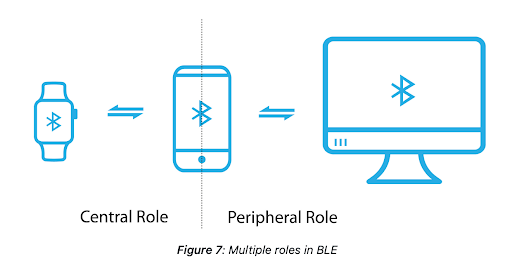
\includegraphics[scale=.7]{centralperipheral.png}
    \label{fig:centralperipheral}
    \end{figure}

\subsection{Piconet}

A piconet is a type of ad hoc network topology that operates without preestablished infrastructure. Devices in a piconet communicate directly with one another without the need for a centralized device like a router or access point. The network is organized with one central device and one or more peripheral devices. A single central can support up to seven active peripherals, while each peripheral can only connect to one central \cite{nextgenBLE}. The central manages the timing and synchronization of all devices in the piconet. Peripheral devices cannot communicate directly with each other; the central acts as a relay, forwarding data between them.

Figure \ref{fig:piconet} shows the structure of a piconet.

\begin{figure}[h]
    \caption{Piconet Topology}
    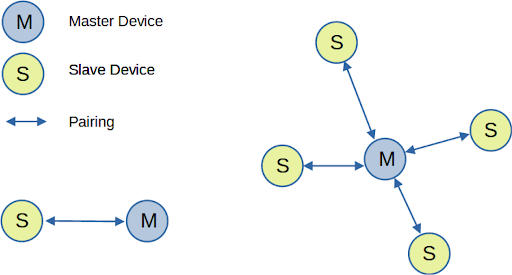
\includegraphics[scale=.7]{piconet.png}
    \label{fig:piconet}
    \end{figure}

All connections made using a BR/EDR controller occur within a piconet. BR/EDR devices communicate over the same physical channel by synchronizing with a shared clock and hopping sequence \cite{bluetoothcorespec6}. The piconet clock follows the central device's clock configuration, and the hopping sequence is also derived from the central’s clock and Bluetooth device address.

Multiple independent piconets can exist in the same area. Each operates on a separate channel and is organized around a different central device. Bluetooth devices can also participate in multiple piconets simultaneously. While a Bluetooth device can only act as the central in one piconet at a time, it can serve as a peripheral in several.


\subsection{Scatternet}

A scatternet is formed by connecting multiple piconets together. Unlike a piconet, a peripheral in a scatternet can connect to multiple central devices. Central devices can also connect to each other, sometimes serving dual roles as both central and peripheral.

For example, a scatternet might include a central laptop connected to a Bluetooth speaker, while also acting as a peripheral to a smartphone and printer. Figure \ref{fig:scatternet} shows a diagram of a typical scatternet. Despite the increased complexity, peripherals still do not communicate directly with each other.

Piconets and scatternets are associated with Classic Bluetooth but are still supported in BLE and later Bluetooth versions \cite{nextgenBLE}. Although BLE—with its advertising mode—has seen growing popularity, traditional Bluetooth methods still offer advantages such as added security during pairing. BLE services enhance the piconet and scatternet model, providing better security, more efficient pairing, and broader support for services.

\begin{figure}[h]
    \caption{Scatteret Topology}
    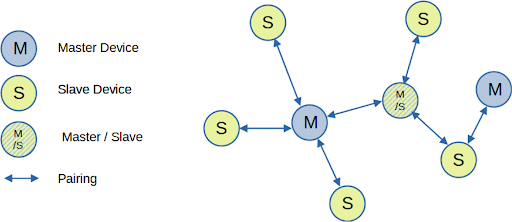
\includegraphics[scale=.7]{scatternet.png}
    \label{fig:scatternet}
    \end{figure}

\section{BLE Mesh Networks}

Mesh networking, introduced with BLE, marks a significant evolution in Bluetooth topologies. In a mesh network, nodes are arranged in a self-configuring mesh, where each node relays traffic between peers when the destination is not directly connected \cite{buildingBLEsystems}.

This structure ensures a reliable path for data packets. If one path is blocked or unavailable, the network reroutes traffic dynamically. The self-organizing nature of mesh networks means they adapt in real-time to changes, such as nodes joining, leaving, or moving within the network.

For example, Figure \ref{fig:mesh} shows Device 1 out of range of Device 3. Device 2, within range of both, acts as a router forwarding messages between them.
\begin{figure}[h]
    \caption{Mesh topology}
    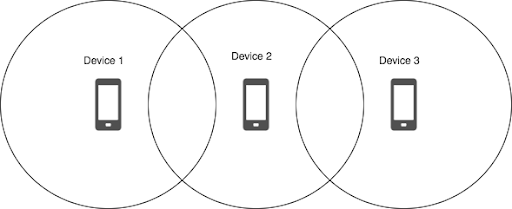
\includegraphics{mesh.png}
    \label{fig:mesh}
    \end{figure}

\section{Broadcast Network from LE}

BLE introduces a new feature called \textit{advertising mode}, which operates differently from the traditional pairing between a central and peripheral. In advertising mode, a device broadcasts data openly to any BLE devices within range that are tuned to the same channel. These listening devices can receive the data and use it as needed—without any pairing, connection, or formal association.

This topology loosely resembles a multi-peripheral piconet, but with a key difference: advertising mode removes the need for a dedicated central or established links. There’s no synchronization or connection—just open broadcasting.

Advertising mode has been a major factor in expanding the possibilities of Bluetooth. By offloading the overhead of pairing, BLE made room for a wider variety of lightweight, low-latency applications. This performance shift is part of why so many modern devices—from smart beacons to virtual reality headsets—are feasible today. Devices like VR headsets, which require fast, efficient data sharing without constant handshaking, would be nearly impossible to build the same way without Bluetooth.

\section{Connections and Mixed Topology}

A connection becomes necessary when data needs to flow in both directions or when there’s more data than can fit into the two available advertising payloads. Connections in BLE are more persistent—they allow devices to remember each other and avoid reestablishing the connection every time. Once established, connections support periodic data exchanges between two devices.

This connection-based pairing is what underpins piconets and scatternets. These connections are private by design: only the two participating devices exchange data (barring external sniffing). As covered earlier, connections involve one central device and one or more peripheral devices.

BLE networks can also incorporate mixed topology configurations depending on the use case. A device that supports both BR/EDR and LE can serve as a bridge between traditional Bluetooth and BLE communication, enabling broader interoperability across protocols. The possibilities for combining these configurations are only constrained by the capabilities of the individual devices' radios and protocol stacks.

Figure \ref{fig:mixedtopology} provides an example of a mixed topology Bluetooth network.

\begin{figure}[h]
    \caption{Mixed Topology}
    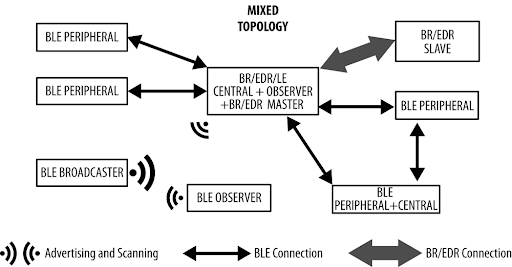
\includegraphics{mixedtopology.png}
    \label{fig:mixedtopology}
    \end{figure}

\section{SCO and ACL Logical Transports}

\subsection{BR/EDR Asynchronous Connection-Oriented (ACL)}

ACL links are the primary way Bluetooth devices using BR/EDR exchange general data. These links handle both control signals (like LMP and L2CAP) and typical user data. ACL is \textit{asynchronous}, meaning data is sent when available rather than on a fixed schedule.

Every Peripheral in a Bluetooth piconet gets one default ACL link to the Central. This link is established when the device first connects and is identified by a Logical Transport Address (LT\_ADDR) assigned by the Central. This LT\_ADDR is also used when identifying the physical connection between devices.

However, because multiple types of logical transports (like SCO links, which are used for voice) might use the same LT\_ADDR, it’s not enough to identify the ACL connection by LT\_ADDR alone. Devices also rely on the packet type to tell them which kind of transport is being used.

ACL links can also carry isochronous data—data that needs to arrive on time, like audio streams—by setting them to automatically drop old packets. At the same time, asynchronous traffic (like file transfers) can still be sent if it’s marked not to auto-flush. This means both types of traffic can share the same ACL link if configured correctly.

If the ACL link is removed or if the device loses sync with the piconet, all other connections between the Central and that Peripheral (like SCO) are also dropped immediately \cite{bluetoothcorespec6}.

\subsection{BR/EDR Synchronous Connection-Oriented (SCO)}

SCO links are designed specifically for real-time data like voice. They create a fixed, circuit-like connection between a Central and a Peripheral by reserving slots on the Bluetooth physical channel. These connections carry 64 kbps of data, usually for audio, and are synchronized with the piconet’s clock.

There are several SCO configurations that balance audio quality, latency, and bandwidth usage. Every SCO connection uses the same LT\_ADDR as the ACL link, so to identify an SCO packet, a device must look at the slot number, packet type, and LT\_ADDR together.

Even though SCO reserves bandwidth, the system can override these slots if higher-priority data (like control messages over ACL) needs to get through. This helps maintain overall system reliability and meet Quality of Service (QoS) requirements.

Unlike ACL links, SCO links don’t carry complex protocols or layered data structures. They just send a steady stream of audio—either in a standard format or as raw data for the application to decode \cite{bluetoothcorespec6}.

\section{Bluetooth Low Energy Broadcasting and Observing}

Bluetooth Low Energy devices communicate with the outside world in two primary ways: \textit{broadcasting} and \textit{connecting}. Both methods are governed by the Generic Access Profile (GAP), which outlines how devices discover and interact with each other \cite{gettingstartedwble}.

Broadcasting enables BLE devices to send data one-way to any scanner or receiver within range. It’s a form of open communication where any nearby device capable of listening can receive the broadcasted data. Figure \ref{fig:broadcastobserve} illustrates this communication model. In the diagram, two roles are shown: the \textit{Broadcaster}, which periodically sends non-connectable advertising packets, and the \textit{Observer}, which continually scans for those packets \cite{gettingstartedwble}.

\begin{figure}[h]
    \caption{Broadcasting and Observing}
    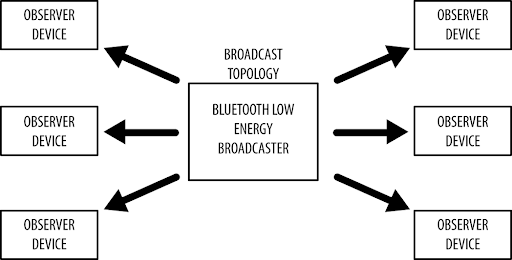
\includegraphics{broadcastobserve.png}
    \label{fig:broadcastobserve}
    \end{figure}

Broadcasting is a key concept in BLE because it’s the only mechanism that allows a device to communicate with multiple other devices simultaneously. This functionality is made possible by BLE’s advertising feature.

A standard advertising packet contains a 31-byte payload, which includes information about the broadcasting device and what it offers. This data can be customized to suit different applications, providing useful context to observing devices. If 31 bytes isn’t enough, BLE allows for a secondary packet called a \textit{Scan Response}, which provides an additional 31 bytes of payload. Observers can request this secondary data if they need more information \cite{gettingstartedwble}.

Broadcasting is quick, efficient, and ideal for sending small amounts of data on a regular schedule to multiple receivers. However, it does come with limitations—particularly around security. Since any device within range can intercept a broadcast, there’s virtually no privacy. Because of this, broadcasting isn’t well-suited for transmitting sensitive or private data.
\section{Bluetooth Protocols and Profiles}

Bluetooth has always had a distinction between protocols and profiles. A protocol is a lower layer foundational block that gets used by all devices that have Bluetooth capabilities. They deal with the layers that implement the different packet formats, routing, encoding, decoding, and multiplexing that allows data to be properly sent between peers \cite{gettingstartedwble}. Profiles are ``vertical slices'' of functionality that encompass either fundamental modes of operation common to all devices (such as the Generic Access Profile and Generic Attribute Profile) or support specific use cases (like the Proximity Profile or Glucose Profile). They essentially define how protocols should be applied to accomplish a particular objective, whether general or specialized.

\section{Bluetooth Low Energy Profiles}

Profiles specify how BLE protocols are to be used to achieve interoperability and support a wide range of applications. These profiles fall into two primary categories: generic profiles, which are fundamental to all BLE operations, and use-case-specific profiles, which are built on top of the generic layers to support particular functionalities.

\subsection{Generic Profiles}

Generic profiles are defined by the Bluetooth Core Specification and provide the foundational mechanisms required for BLE communication. These profiles ensure that devices from different manufacturers can interoperate seamlessly. Two such profiles—Generic Access Profile (GAP) and Generic Attribute Profile (GATT)—are mandatory for all BLE-compliant devices and serve as the cornerstones of BLE communication.

\subsubsection{Generic Access Profile (GAP)}

The Generic Access Profile defines the roles, procedures, and operational modes required for device discovery, broadcasting, connection establishment, connection management, and security negotiation. GAP operates as the top-level control layer within the BLE protocol stack, orchestrating the basic behaviors necessary for device interaction. All BLE devices must implement and conform to the GAP specifications to ensure compatibility and reliable communication.

\subsubsection{Generic Attribute Profile (GATT)}

GATT focuses primarily on how data is exchanged. GATT defines a universal data model and a set of procedures that enable devices to discover, read, write, and notify data values. It functions as the uppermost data layer in BLE and serves as the foundational framework upon which most BLE applications and services are constructed.

Due to their foundational roles, GAP and GATT are commonly exposed through application programming interfaces (APIs), making them the primary entry points for developers interacting with the BLE protocol stack.

\subsection{Use-Case-Specific Profiles}

Beyond the generic profiles, the Bluetooth Special Interest Group (SIG) has defined a series of use-case-specific profiles. These profiles are designed to standardize behavior for specific applications and are exclusively built upon the GATT framework. At the time of writing, no BLE profiles exist outside the GATT structure. However, the introduction of connection-oriented L2CAP channels in Bluetooth version 4.1 may pave the way for future GATT-less profiles.

\subsubsection{SIG-Defined GATT-Based Profiles}

The Bluetooth SIG provides an extensive catalog of standardized profiles, each tailored to support a specific application or device type. These profiles fully specify the required procedures and data formats, facilitating rapid development and ensuring interoperability across implementations.

Examples of SIG-defined GATT-based profiles include:

\begin{itemize}
    \item \textbf{Find Me Profile:} Enables physical location of nearby BLE devices (e.g., locating a lost phone or keyring).
    \item \textbf{Proximity Profile:} Detects when a connected device moves beyond a designated range, triggering alerts.
    \item \textbf{HID over GATT Profile:} Facilitates the transmission of Human Interface Device (HID) data over BLE for peripherals such as keyboards, mice, and remote controls.
    \item \textbf{Glucose Profile:} Securely transmits glucose measurement data for health monitoring applications.
    \item \textbf{Health Thermometer Profile:} Enables transfer of body temperature readings from wearable or medical devices.
    \item \textbf{Cycling Speed and Cadence Profile:} Allows cycling sensors to relay speed and cadence information to companion applications or devices.
\end{itemize}

A comprehensive list of SIG-adopted profiles is available on the Bluetooth SIG Specification Adopted Documents webpage. Developers may also consult the Bluetooth Developer Portal for up-to-date listings of adopted services and characteristics.

\subsubsection{Vendor-Specific Profiles}

While the SIG provides a broad range of standardized profiles, the BLE specification also permits the definition of vendor-specific profiles. These profiles are often developed to support proprietary use cases not covered by SIG standards. Vendor-specific profiles can be implemented privately between two devices (such as with a health accessory and a smartphone) or published to enable broader adoption.

Notable examples of vendor-defined profiles include:

\begin{itemize}
    \item \textbf{Apple iBeacon:} A proprietary proximity-sensing profile used for indoor positioning and location-based services.
    \item \textbf{Apple Notification Center Service (ANCS):} Enables wearable devices or external displays to access and display iOS notifications.
\end{itemize}

These profiles demonstrate the flexibility of the BLE specification in accommodating both standardized and proprietary communication models.

\section{Bluetooth Low Energy (BLE) Architecture}

Although most users will only ever interact with the top layers of the Bluetooth Low Energy (BLE) protocol stack, having a basic understanding of the full stack can provide helpful context. This overview lays the groundwork for understanding how BLE devices work and why each part of the system is important. A typical single-mode BLE device is made up of three main parts: the controller, the host, and the application. Each of these parts contains multiple layers, each responsible for specific tasks that allow the device to communicate and perform its intended functions. Figure \ref{fig:bleprotocolstack} shows the BLE protocol stack.

\begin{figure}[h]
    \caption{BLE Protocol Stack}
    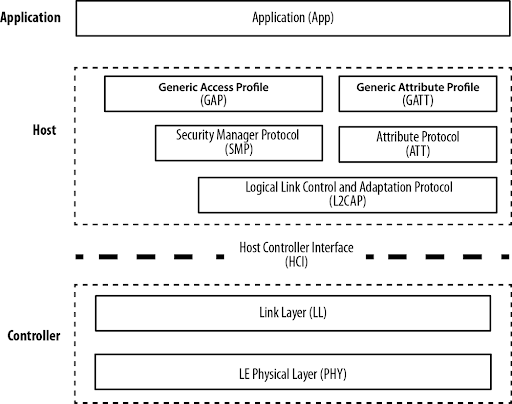
\includegraphics[scale=.7]{bleprotocolstack.png}
    \label{fig:bleprotocolstack}
    \end{figure}

\subsection{Application}

The application layer sits at the top of the BLE protocol stack. It includes all the logic, data handling, and user interface components that define how a device behaves in a specific use case. This layer is highly customized and varies from one implementation to another \cite{nextgenBLE}.

\subsection{Host}

Below the application is the host, which includes several critical layers that manage communication and device behavior:

\begin{itemize}
    \item \textbf{Generic Access Profile (GAP):} Controls how devices advertise themselves, discover others, establish connections, and manage roles and security \cite{nextgenBLE}.
    \item \textbf{Generic Attribute Profile (GATT):} Organizes and manages how data is exchanged between connected devices.
    \item \textbf{Logical Link Control and Adaptation Protocol (L2CAP):} Handles multiplexing and segmentation of data packets.
    \item \textbf{Attribute Protocol (ATT):} Supports data operations such as reads and writes via attribute handles.
    \item \textbf{Security Manager (SM):} Manages pairing, authentication, and encryption.
    \item \textbf{Host Controller Interface (HCI) – Host Side:} Facilitates communication between the host and controller \cite{nextgenBLE}.
\end{itemize}

\subsection{Controller}

At the bottom of the Bluetooth stack, the controller is responsible for radio operations and low-level data transport. It typically includes the following components:

\begin{itemize}
    \item \textbf{Physical Layer (PHY):} Manages the actual transmission and reception of radio signals.
    \item \textbf{Link Layer (LL):} Controls advertising, scanning, and maintaining connections.
    \item \textbf{HCI (Controller Side):} Complements the host side of HCI to enable structured data flow between layers \cite{nextgenBLE}.
\end{itemize}

According to the Bluetooth Core Specification, a Bluetooth implementation includes a single controller, which may be configured as one of the following:

\begin{itemize}
    \item A \textbf{BR/EDR controller}, containing the Radio, Baseband, Link Manager, and optionally HCI.
    \item An \textbf{LE controller}, including the LE PHY, Link Layer, and optionally HCI.
    \item A \textbf{dual-mode controller} that combines both BR/EDR and LE controller functions into a single unit.
\end{itemize}

Together, these layers ensure that BLE devices can connect reliably and communicate efficiently. This layered architecture is often described from the bottom up — starting at the antenna and PHY layer and moving up through the stack to the user-facing application.

\section{BLE Link Layer and Device Addressing}

In the Bluetooth Low Energy (BLE) protocol stack, the Link Layer serves as a crucial interface between the Physical Layer—which handles the actual radio transmission—and the upper protocol layers. It acts as the controller for radio operations and is essential for managing the states and timing mechanisms that define BLE communication. One of the key responsibilities of the Link Layer is to abstract the radio hardware, allowing higher-level layers to interact with it through the Host Controller Interface (HCI) \cite{introtoble}. 

In addition to timing and control, the Link Layer manages several hardware-accelerated tasks. These include generating cyclic redundancy checks (CRC) for error detection, producing random numbers for cryptographic operations, and performing encryption to secure data transfer \cite{introtoble}. These operations ensure the performance, integrity, and security of BLE communications.

\subsection{Link Layer States}

BLE devices operate in a well-defined set of five main states, each with specific behaviors and transitions:

\begin{itemize}
    \item \textbf{Standby:} This is the default state, where the radio is idle and not transmitting or receiving any packets.
    \item \textbf{Advertising:} In this state, the device broadcasts data packets at regular intervals, making itself discoverable to other devices.
    \item \textbf{Scanning:} Devices in this state listen for advertising packets from others, searching for devices they might want to connect with.
    \item \textbf{Initiating:} When a scanning device decides to connect to an advertising device, it enters this state and sends a connection request.
    \item \textbf{Connected:} A persistent communication link is established. Devices in this state can exchange data regularly. The device that initiated the connection becomes the master, while the other becomes the slave \cite{introtoble}.
\end{itemize}

This framework enables BLE to support dynamic and responsive device discovery and communication, while keeping energy consumption minimal.
\section{Advertising, Scanning, and Connecting}

Advertising and scanning are complementary operations: advertising devices periodically transmit small packets of data, while scanning devices listen for and interpret these packets. If the advertiser allows connections, and a scanning device decides to initiate one, both devices transition into the connected state \cite{introtoble}. These processes form the backbone of BLE interactions and are covered in more depth in subsequent chapters of most BLE technical literature.

\section{Bluetooth Device Address}

Every Bluetooth device is identified by a 48-bit device address, which serves a function similar to a MAC address in networking. BLE supports two major types of device addresses: public addresses and random addresses, which influence how discoverable and trackable a device is.

\subsection{Public Address}

A public address is a globally unique, fixed identifier that is factory-programmed and registered with the IEEE. Because of this registration requirement, it ensures uniqueness across all BLE devices worldwide. However, it can also present privacy concerns, since it does not change and is easily traceable \cite{introtoble}.

\subsection{Random Address}

Random addresses, by contrast, provide more flexibility and are often preferred in consumer devices to protect user privacy. These addresses can either be static or private, and they do not require IEEE registration.

\begin{itemize}
    \item \textbf{Static Address:} Used as a drop-in replacement for public addresses. A static address remains the same between sessions but can be regenerated at boot or kept for the lifetime of the device until a power cycle occurs.
    \item \textbf{Private Addresses:} These are designed to change regularly and enhance privacy. They come in two subtypes:
    \begin{itemize}
        \item \textbf{Non-resolvable private addresses} are temporary, randomly generated, and cannot be traced back to a specific device. They are rarely used due to limited functionality.
        \item \textbf{Resolvable private addresses} use an Identity Resolving Key (IRK) and a random number to generate temporary addresses. These change over time, making the device hard to track by unknown parties. However, trusted or bonded devices that have the IRK stored can resolve these addresses, allowing them to re-identify the device securely \cite{introtoble}.
    \end{itemize}
\end{itemize}

This system allows BLE to balance two key goals: persistent connectivity with trusted devices and protection against unwanted tracking or eavesdropping by unknown entities.

\section{Host Controller Interface (HCI) Layer}

The Host Controller Interface (HCI) serves as the communication bridge between the host and controller layers in a Bluetooth system. These components can be implemented on the same chipset or on separate chipsets. When they are on separate chipsets, HCI is critical for enabling interoperability and communication between them. In such cases, HCI defines both the standardized protocol and the physical transport mechanisms that facilitate message exchange. As shown in Figure \ref{fig:hosthcicontroller}, the host, HCI, and controller are depicted as distinct components. HCI commonly uses transport technologies such as UART, USB, and SDIO to establish physical connections between the host and controller. When the host and controller are integrated on the same chipset, HCI functions as a logical interface rather than a physical one \cite{introtoble}.

\begin{figure}[h]
    \caption{Host, HCI, and Controller components}
    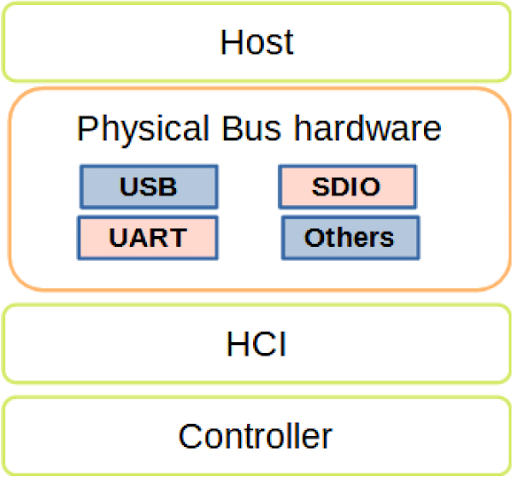
\includegraphics[scale=.6]{hosthcicontroller.png}
    \label{fig:hosthcicontroller}
    \end{figure}

\subsection{Universal Asynchronous Rx/Tx (UART)}

UART is a serial communication protocol that uses wired connections to exchange data between devices. It is commonly found in integrated circuits and is especially favored in devices like mobile phones and laptops, where the entire Bluetooth stack is implemented on a single chipset. UART is also well-suited for small, resource-constrained devices powered by microcontrollers, as it is lightweight and efficient in its use of system resources \cite{nextgenBLE}.

In the context of the HCI UART protocol, four types of packet transmissions are defined: the Command packet (identified by 0x01), Event packet (0x04), Asynchronous Connection-Less (ACL) packet (0x02), and Synchronous Connection-Oriented (SCO) packet (0x03). Because the receiving HCI layer cannot distinguish these packet types based on content alone, each transmission begins with a leading byte — known as an indicator — which acts as a header to identify the type of packet that follows \cite{nextgenBLE}.

\section{Connection}

To establish a connection in Bluetooth Low Energy (BLE), the central device begins by scanning for advertising peripheral devices that are currently accepting connection requests. Advertising packets can be filtered based on the Bluetooth Address or the contents of the advertising data itself. Once a suitable advertiser is detected, the master sends a connection request packet. If the slave responds, a connection is established \cite{gettingstartedwble}.

This connection request packet includes several critical parameters:
\begin{itemize}
    \item \textbf{Frequency hop increment:} Defines the hopping sequence used for the duration of the connection.
    \item Three additional connection parameters:
    \begin{itemize}
        \item \textbf{Connection interval:} The time between the start of two consecutive connection events. This can range from 7.5 ms (for high throughput) to 4 seconds (for minimal power usage).
        \item \textbf{Slave latency:} The number of connection events the slave is allowed to skip without causing a disconnection.
        \item \textbf{Connection supervision timeout:} The maximum allowed time between receiving valid packets before the connection is considered lost \cite{gettingstartedwble}.
    \end{itemize}
\end{itemize}

Once connected, communication happens through repeated connection events — periodic time slots where the master and slave take turns exchanging packets. A connection event:
\begin{itemize}
    \item Always begins with a packet from the central.
    \item Requires the peripheral to respond if it receives a packet.
    \item Continues until both sides have no more data to send.
    \item Is repeated at the connection interval until the connection is either closed or lost.
    \item Can be closed by either the master or the slave. If the central sends a packet and does not receive a response, it waits until the next connection event to resume \cite{introtoble}.
\end{itemize}

To manage interference and ensure privacy or security, BLE supports a white list mechanism at the Link Layer. This list defines which Bluetooth device addresses are of interest. Devices not on the list are ignored — their advertising (by scanners) or connection request packets (by advertisers) are simply dropped \cite{gettingstartedwble}.

\section{Services and Characteristics}

\subsection{Attribute Protocol (ATT)}

The Attribute Protocol (ATT) defines how a server exposes its data to a client, and how that data is organized and accessed in a Bluetooth Low Energy (BLE) system \cite{introtoble}.

\subsubsection{Roles in ATT}

There are two main roles in ATT communication:
\begin{itemize}
    \item \textbf{Server:} The server is the device that stores and exposes data, and may allow certain behaviors to be remotely controlled. It receives commands from peer devices and sends responses, notifications, or indications in return. For example, a thermometer acts as a server when it provides access to its current temperature, unit of measurement, battery level, or the interval at which it records readings. Instead of requiring the client to repeatedly poll for changes, the server can proactively notify the client when data updates occur \cite{introtoble}.
    \item \textbf{Client:} The client is the device that reads data from the server or controls the server's behavior. It sends commands and requests, and accepts incoming notifications and indications. In the thermometer example, a mobile device that connects to the thermometer and reads temperature values is operating as the client \cite{introtoble}.
\end{itemize}

\subsubsection{Data Format: Attributes}

The data exposed by the server is organized into attributes. An attribute is a general term for any piece of data available on the server, such as services or characteristics (described later).

Each attribute consists of the following elements:
\begin{itemize}
    \item \textbf{Attribute Type (UUID):} This is a Universally Unique Identifier (UUID) used to distinguish the type of data.
    \begin{itemize}
        \item A 16-bit UUID is used for Bluetooth SIG-adopted attributes.
        \item A 128-bit UUID is used for custom or vendor-specific attributes defined by developers \cite{introtoble}.
    \end{itemize}
    \item \textbf{Attribute Handle:} This is a 16-bit value that acts like an address assigned by the server to each of its attributes. The handle uniquely identifies an attribute during the lifetime of the connection, allowing the client to reference it directly. Handle values range from 0x0001 to 0xFFFF, while 0x0000 is reserved \cite{introtoble}.
    \item \textbf{Attribute Permissions:} Permissions control whether an attribute can be read, written, notified, or indicated, and what security requirements are necessary for each operation. These permissions are not specified within ATT itself, but are defined at a higher layer—typically the GATT (Generic Attribute Profile) or application layer \cite{introtoble}.
\end{itemize}
\section{Profiles}

\subsection{Generic Attribute Profile (GATT)}

The Generic Attribute Profile (GATT) defines how BLE devices organize, expose, and exchange data over a connection. It builds directly on top of the Attribute Protocol (ATT), using it as the transport layer for transmitting structured data known as attributes \cite{introtoble}.

GATT introduces a hierarchical data model centered around three key concepts:
\begin{itemize}
    \item \textbf{Services}
    \item \textbf{Characteristics}
    \item \textbf{Profiles} \cite{introtoble}
\end{itemize}

These elements allow BLE devices to encapsulate user-facing data and device functionality in a standardized, interoperable way. All BLE application-level interactions happen within the framework defined by GATT \cite{gettingstartedwble}.

\subsection{GATT Roles}

Like ATT, GATT supports client and server roles, which are dynamic per transaction rather than fixed per device. This means a single device can simultaneously act as a GATT server for one connection and a GATT client in another \cite{introtoble}.

\begin{itemize}
    \item \textbf{GATT Server:} Stores and exposes attributes to the client. It responds to requests and may send unsolicited updates via notifications or indications. Every BLE device must at least support a minimal GATT server, even if only to respond with error codes \cite{gettingstartedwble}.
    \item \textbf{GATT Client:} Initiates communication by performing service discovery, reading/writing attributes, and subscribing to updates. The client has no prior knowledge of the server’s structure—it learns through discovery procedures \cite{gettingstartedwble}.
\end{itemize}

\subsection{Services}

A service is a logical grouping of one or more attributes that collectively provide a certain function on the server. A service always includes at least one characteristic, and often contains supporting attributes like declarations, descriptors, and included services (used to reference other services) \cite{introtoble}.
\begin{itemize}
    \item \textbf{Primary Services:} Represent core functionality (e.g., Battery Service).
    \item \textbf{Secondary Services:} Offer auxiliary support and must be referenced by primary services (rarely used) \cite{introtoble}.
\end{itemize}

The Bluetooth SIG maintains a set of adopted services with published specifications to ensure interoperability across vendors. If a product claims compliance with one of these services, it must strictly follow its specification \cite{introtoble}.

\subsection{Characteristics}

A characteristic is the smallest logical unit of user-accessible data on a BLE server. It always belongs to a service and includes:
\begin{itemize}
    \item \textbf{Value:} The actual data being exposed.
    \item \textbf{Properties:} Operations permitted on the value (e.g., read, write, notify, indicate).
    \item \textbf{Descriptors:} Metadata about the value (e.g., format, units, configuration settings) \cite{introtoble}.
\end{itemize}

For example, the battery level characteristic within the Battery Service lets clients read the device's current power level \cite{introtoble}.

\subsection{Profiles}

While services and characteristics define how data is stored and exposed on the server, profiles describe how clients and servers interact, including service usage, connection procedures, and security requirements. Profiles are not discovered over BLE connections like services are; instead, they exist as specification documents, often adopted by the Bluetooth SIG. These define how multiple services should be used together to achieve specific use cases (e.g., Heart Rate Profile, Blood Pressure Profile) \cite{introtoble}.

Each profile specification includes:
\begin{itemize}
    \item Required services and characteristics
    \item Interaction behaviors for both server and client
    \item Connection and security requirements
    \item Example usage diagrams and workflows \cite{introtoble}
\end{itemize}

\section{Nordic Semiconductor}

\subsection{nRF Connect}

nRF Connect for Mobile—formerly known as the nRF Master Control Panel—is a feature-rich application designed for developers working with Bluetooth Low Energy (BLE) devices. Created by Nordic Semiconductor, this free app is available on both Android and iOS platforms and is widely regarded as one of the most powerful tools for BLE development and testing \cite{buildingBLEsystems}.

The application supports numerous Bluetooth SIG-adopted profiles, including Over-the-Air Device Firmware Updates (OTA DFU), making it especially useful for firmware deployment and debugging \cite{buildingBLEsystems}.

\subsubsection{Key Features} \cite{buildingBLEsystems}:
\begin{itemize}
    \item \textbf{BLE Device Scanning with RSSI Graphs:} Visualize signal strength (RSSI) for nearby devices in real-time.
    \item \textbf{Advertisement Data Parsing:} Inspect general advertisements and manufacturer-specific payloads.
    \item \textbf{GATT Client Functionality:} Connect to BLE peripherals and display their services and characteristics.
    \item \textbf{Characteristic Interaction:} Perform reads, writes, and observe values from server-side characteristics.
    \item \textbf{Support for Notifications and Indications:} Enable and receive updates directly from connected devices.
    \item \textbf{GATT Server Emulation:} Simulate a GATT server with built-in configuration presets.
    \item \textbf{OTA Firmware Updates:} Flash firmware over-the-air for supported devices.
    \item \textbf{Automated Testing:} Execute test cases defined in XML scripts for BLE device behavior validation.
    \item \textbf{UART Service Support:} Communicate via UART-over-BLE channels.
\end{itemize}

\subsubsection{Compatibility:}
\begin{itemize}
    \item \textbf{Android:} Version 4.3 and higher
    \item \textbf{iOS:} Version 8.0 and higher
\end{itemize}

With its comprehensive feature set, nRF Connect is an essential tool for BLE developers, from prototyping and debugging to final deployment \cite{buildingBLEsystems}.



%!TEX root = ../main.tex

\chapter{Reverse Engineering}

\section{Analysis Methods and Tools}
\subsection{Static Analysis}
Static analysis is a practice of analyzing code without executing it. 
It can  be used to help inform dynamic analysis. 
Static analysis tools can analyze at either the source code level with code that hasn’t been compiled yet or machine language level with code that has. 
Static analysis tools can be used by reverse engineers to retrieve and comb over assembly level code.
This is one of the most basic functions of any static analysis tool, but many of them offer a lot more functionality to help reverse engineers. 
Most static analysis tools are designed to help give the reverse engineer a starting off point with interpreting assembly level functions.

\subsubsection{Disassembler}
One of the most key static analysis tools for a reverse engineer is a disassembler. 
Disassemblers are applications that take in a program’s executable file and generate a file with the assembly code.
This isn’t too difficult because assembly is just a text translation of the machine readable binary code. 
Unfortunately, that makes it a lot less clear than higher level programming languages.  
Disassembly is also unique to a person’s processor, but there are disassemblers that can support more than one CPU architecture.
Some examples of disassemblers are IDA, Binary Ninja, Hopper, Ollydbug, Radare2, and Ghidra.

\subsubsection{Decompiler}
Decompilers are similar but more complex than disassemblers.
 Instead of just producing the assembly language code, decompilers attempt to produce high-level readable code. 
 They attempt to produce something that looks as close to the source code as possible by reversing the compilation process~\cite{Reversing}. 
 The front end of the decompiler decodes low-level assembly instructions and translates it into an intermediate representation specific to the decompiler. 
 The intermediate representation is then iterated on to remove as many extraneous details as possible while preserving the important details. 
 Lastly the back end takes the polished up intermediate representation and translates it again into a high level language.

While this may sound like a simple way to retrieve the source code, it is highly unlikely the high level language returned will be something that actually matches. 
Anyone who has ever run text through a translation website multiple times knows that each iteration causes a loss in fidelity and oftentimes the end result will be gibberish. 
Decompilers go a step further and have no immediate knowledge of things like function or variable names and structures. 
This does not make them useless, though. For example, a text translator will usually return your original result when given a simple phrase. 
Similarly a decompiler will most likely be able to pick up on more straightforward functions such as adding a + b. 
Decompilers offer hints and snippets into what the source code may look like which is valuable information for a reverse engineer. 
Most of the examples for disassemblers listed also count as decompilers.

\subsubsection{Dumping Tools}
Executable dumping is usually the first step in reverse engineering a program. 
Executable dumping helps inform a reverse engineer what a program does, how it interacts with external elements, and general knowledge of how a file is structured. 
Using dumping tools, a reverse engineer will start by figuring out what type of file they’re dealing with. 
They will then start to unpack the format. 
Extracting strings will immediately offer insight into what language the source code is written in, what library modules it uses, what kinds of data it is dealing with, and what the goals of program functions may be. 
Other useful information we can retrieve is the layout of the file in memory and what the general logical structure of the file is. Once we know the type of file we also know which tools we can use. 
For example, some debuggers only work with certain high and low level languages. 
Some popular executable dumping programs are ones already built into your machine like DUMPBIN for windows or otool for mac. 

Otool is identifies a file's mach header. 
On systems with a Mach kernel like macOS and iOS, the executable binaries they use will have a mach header. 
All headers have a magic number to identify them. T
hin binaries only have that number while fat binaries with fat headers will have locations of the other executable's headers in them

\subsection{Dynamic Analysis}
Dynamic Analysis occurs when the program or section being analyzed is run during the analysis process. 
Because dynamic analysis requires the program to execute with unknown results, it is safest to do it in an enclosed or sandboxed environment to protect the rest of the system. 
Thus easily manipulated virtual machines are usually set up during the dynamic analysis process.
Many tools can be part of the dynamic analysis process. 
Anything that needs to run and monitor some output is considered dynamic. 
Tools may run the full program, a portion of the program, or even just a single line. 
Tools that monitor the external environment while the program runs are also considered dynamic.

\subsubsection{Debugger}
Debuggers are a tool usually used for developers to locate and work through errors in their programs, but they’re also vital tools in reverse engineering. 
Many debuggers can work through assembly language. 
While assembly language may be difficult for a human to parse through, it is the exact same logic that gets broken down and sent to a computer meaning that the computer can show what each assembly instruction is intended to do. 
Most debuggers software engineers use were actually designed from the ground up with the purpose of stepping through assembly code. 
The debugger can show the state of CPU registers along with a memory dump that shows what’s in the stack. 
Debuggers usually contain disassemblers which as discussed is a vital reverse engineering tool. 
Many debuggers also contain both software and hardware breakpoints. 
Software breakpoints are instructions added into the code during runtime to pause and hand control over to the debugger. 
Hardware breakpoints are a CPU feature which allow the processor to pause execution when a certain memory address is reached and hand control over to the debugger. 
A reverse engineer can use insert breakpoints at data structures of interest and use the debugger to reveal what they are. 
Debuggers also offer a clear view of registers and memory to aid in a reverse engineer's ability to process low level information.

\paragraph{\underline{User Mode Debuggers}}
Most debuggers that a programmer will use are user mode debuggers. 
They run on a system like any other application then seize control of the target program to debug ~\cite{Reversing}.
An advantage to them is that they are easier to set up and navigate than their kernel-mode counterparts.
Usually it’s fine to stay limited to user mode viewing of an application. 
It only creates troublesome limitations when the target application has kernel mode components such as device drivers. 
User mode debuggers are also not always sufficient when trying to debug a program before it reaches the main entry point. 
These kinds of programs are usually ones that have a lot of statically linked libraries in the executable. 
The final and most likely to be problematic issue is that user-mode debuggers can only view a single process in a program. 
This can cause issues when the target application has processes that interact in unknown ways. 
The user may not know which process to zero in on that has the code of interest.

\paragraph{\underline{Kernel Mode Debuggers}}
Kernel mode debuggers are different from user-mode debuggers because they capture the entire system and not just a single process. 
Instead of running atop the operating system, kernel mode debuggers sit alongside the system kernel and stay ready to capture the entire system’s stats. 
Kernel mode debuggers can be more helpful to reverse engineers because they offer more clues as to what’s going on with the system. 
A key tool for kernel-mode debuggers is that they allow the placement of low level code breakpoints. 
As a reverse engineer working with assembly code, being able to test different sets of assembly instructions that may be the code section a reverser is looking for is incredibly useful.

For example, picture a scenario where a reverse engineer is looking for the API responsible for handling moving windows? 
That will need to be managed by a windows manager in the kernel. 
The complexity is introduced when trying to identify which API moves a particular window. 
Since there are multiple APIs that can be used to move a window, pinpointing the one you are trying to focus on is a difficult task. 
This is where kernel mode debuggers come in handy. 
Low level breakpoints in the operating system responsible for shifting windows around will help you identify which API is getting called when a window is moved~\cite{Reversing}. 
From there the reverse engineer will be able to hone in on that API.

Unfortunately, kernel mode debuggers come with their own drawbacks. 
Setting them up can be challenging because they require access to the full system. 
They need to suspend the entire system while running so they can go line by line, which means the system can no longer have multiple threads going~\cite{Reversing}. 
They will also usually need to be set up inside a Virtual Machine which will be discussed in a later section~\cite{PracticalRE}. 
These are reasons why a reverser should exhaust their other options before jumping into using a kernel mode debugger. 
Still, they are powerful tools when the scenario calls for it.

\subsubsection{System Monitor}
System monitoring can be a crucial part of the reverse engineering process. 
In some cases, a reverse engineer can figure out what they need through system monitoring tools without ever looking at the decompiled code. 
System monitoring tools can capture what happens between the code and hardware using the intermediate channels of input/output~\cite{Reversing}. 
For local system monitoring, tools monitor things such as file operations (creating, deleting, moving, etc). 
For programs that communicate over networks, system monitoring might look like recording all TCP/UDP network traffic. 
System monitoring tools are commonly used in virtual machines.


\subsubsection{Virtual Machine}
Many programmers will encounter virtual machines (VM) at some point during their career. 
It’s not uncommon for an application to interface exclusively with one type of operating system. 
One reason is because writing applications to work with different operating systems adds time and complexity that not all programmers can afford.
Choosing to write in a high level language may make code more portable because there’s more verbose built-in libraries or interpreters that deal with the specifics of the systems without the need for any programmer intervention.
But high level languages often trade performance for convenience which is not a trade that a developer working with large amounts of data can necessarily afford to take.
What happens when a developer has an application that runs on Windows while they have a Mac? 
This is where a virtual machine enters into the mix. Virtual machines are safe sandboxed environments that work as miniature computers with their own operating systems within a computer. 
They are constructed with an interpreter and bytecode. 
During compile time, select code snippets are compiled specific for the VM target architecture and then inserted into the program along with the interpreter. 
During run-time, the interpreter begins executing the bytecode. 
Virtual machines are costly to implement because they are so expansive which is why only the necessary code snippets get rendered~\cite{MasteringRE}.
Because virtual machines work in their own isolated environment, they offer powerful protections against unknown or potentially malicious software. 
This makes them a useful tool for reverse engineers who deal with software that they do not know the contents of. 
The level of control over virtual machines also makes them a useful tool because there is ultimate knowledge of system conditions.


\section{Compiled Code RE}
It is important for a reverser to understand the different goals of high level and low level languages. 
Understanding these differences will help with interpretation of why code is structured a certain way.


\subsection{High level languages}
High level languages exist to take away the complexity of system specific programming.
High level languages work so that a programmer can focus on specifying the clean structural logic without needing to dedicate time to figuring out system specific details. 
While writing in something like assembly can be very performative, it would be nearly impossible for a standalone human to write a modern application in assembly.
Because high level languages favor simplicity over the flexibility to do exactly what is the most efficient for achieving a program’s goals, many programmers don’t even know what is going on at the assembly level. 
A reverse engineer will be forced to pick apart what potentially roundabout ways a program’s goals are being achieved. 
The main goal of a reverse engineer is to use what they know about what the program was trying to do, potential ways that can be accomplished in high level code, and how to read assembly code to make their best educated guess on what’s happening where.
For reverse engineers, the most important thing to know about a high level language is to what level does it abstract or conceal the underlying machine code~\cite{Reversing}. 
Languages like Python that have a built in interpreter will abstract it a lot. 
These programs may be full of extraneous machine code. On the other hand, languages like C are written much closer to the target processor and won’t have nearly as much separation between the source and machine code.

\subsubsection{Control Flow}
Control flow is what makes code more user friendly. 
This manifests through statements like conditionals that give general instructions for what a program should do when. '
A processor has no knowledge what statements like ‘if’ or ‘while’ mean. 
Under the hood, these statements translate into verbose and daunting assembly code. 
This is because high level conditional statements are often broken down into operation sequences because it would otherwise overwhelm the processor~\cite{Reversing}.

Other typical structural components of programs that aid in control flow are switch blocks and loops. 
Switch blocks, or \(n-way\) conditionals, take in an input and have \(n\) number of code blocks that are potentially executed depending on the input value. 
Each block of code gets assigned at least one value prior to runtime. 
The compiler also generates code to receive the input value and search for the proper code block to execute. 
The values for the code blocks are usually stored in a lookup table that has pointers to each corresponding code block.  
Depending on the input value, the program will go through the process of searching the lookup table then jumping to the proper code block at runtime~\cite{Reversing}. 
Loops work to allow a program to repeatedly execute a certain code block multiple times. A loop has a counter to keep track of how many iterations it has performed. 
There is also a conditional statement that determines when the loop will stop. 
Loops and conditionals are inherently intertwined. 
The difference is that loops execute over and over until the condition is no longer met.

To understand control flow sequences, one must understand how low level control flow is implemented. 
This means that a reverse engineer needs to know the specific rules of each kind of low level architecture because low level control flow is individual to the platform and therefore the language.

\subsection{Low level languages}
Earlier we mentioned that complexity is introduced when working with low level system specific details. 
This is especially true when the goal is to translate high level logic into something that will be understood by your machine. 
Of course, there must be a way to do this because the CPU does it anytime a modern application is run. 
But it often involves keeping track of more details than a sole human is capable of. 
That is why a reverse engineer must develop the skill of parsing through assembly code and being able to create a kind of ‘mental image’ of how it relates to high level constructs.
Data management is one of the things that a person’s computer keeps track of that would be difficult for a human to do.
 To understand why this is, we can look at the data management of a relatively low level language, C, versus the assembly representation. 
 Consider the code: 
\begin{lstlisting}

int divide(int a, int b) {
    int result;
    result = a // b;
    return result;
}
\end{lstlisting}
While this function may seem incredibly simple, there is no direct translation into a machine code representation. 
To execute this in a low level language, it would require first storing the machine state. 
Then memory would need to get allocated for result. Variables a and b would need to get loaded from memory into a register. 
Then a would need to be divided by b and the result would need to get stored in the register that got loaded in the beginning. 
The machine state from before would need to get reloaded. The pointer would need to return to the caller and bring back result~\cite{Reversing}.
One line of high level code could result in any number of assembly instructions.
Managing data is one of the biggest challenges of reverse engineering.


\subsubsection{Registers}
To keep from needing to constantly access RAM, microprocessors have a smaller internal memory that can be accessed with barely any performance cost~\cite{Reversing}. 
There are multiple types of internal memories that microprocessors keep and registers are one of them.
Registers are little pieces of internal memory that live within the processor and are able to be accessed with an imperceptible cost to performance~\cite{PracticalRE}.
The biggest problem with registers is that there are not very many of them. 
One of the most popular processors, the IA-32, only has eight 32-bit registers that can be used for anything. 
It does have more registers, but they all have highly specific use cases. 
Assembly language is written around utilizing registers because they’re so performant. 
They are not good for long term storage, though, that is when RAM becomes the better choice. 
One of the most important things to take away is that CPUs do not automatically manage this. 
Data management is outlined in the assembly code which is what reverse engineers will need to get comfortable sorting through.

One thing that reverse engineers will need to do is focus on figuring out what kind of values are getting loaded into a register. 
For example, it is easy to see when a register is only being used to grant instructions access to a specific value because that register will only show up when transferring value from memory to the instruction or vice versa.
Another example is when a register shows up many times in one function. 
This is a good clue that one of the function's local variables is being stored in that register.
\begin{figure}[h]
    \caption{Figure modified using Intel® 64 and IA-32 Architectures Software Developer’s Manual and https://flint.cs.yale.edu/cs422/doc/pc-arch.html\#register}
    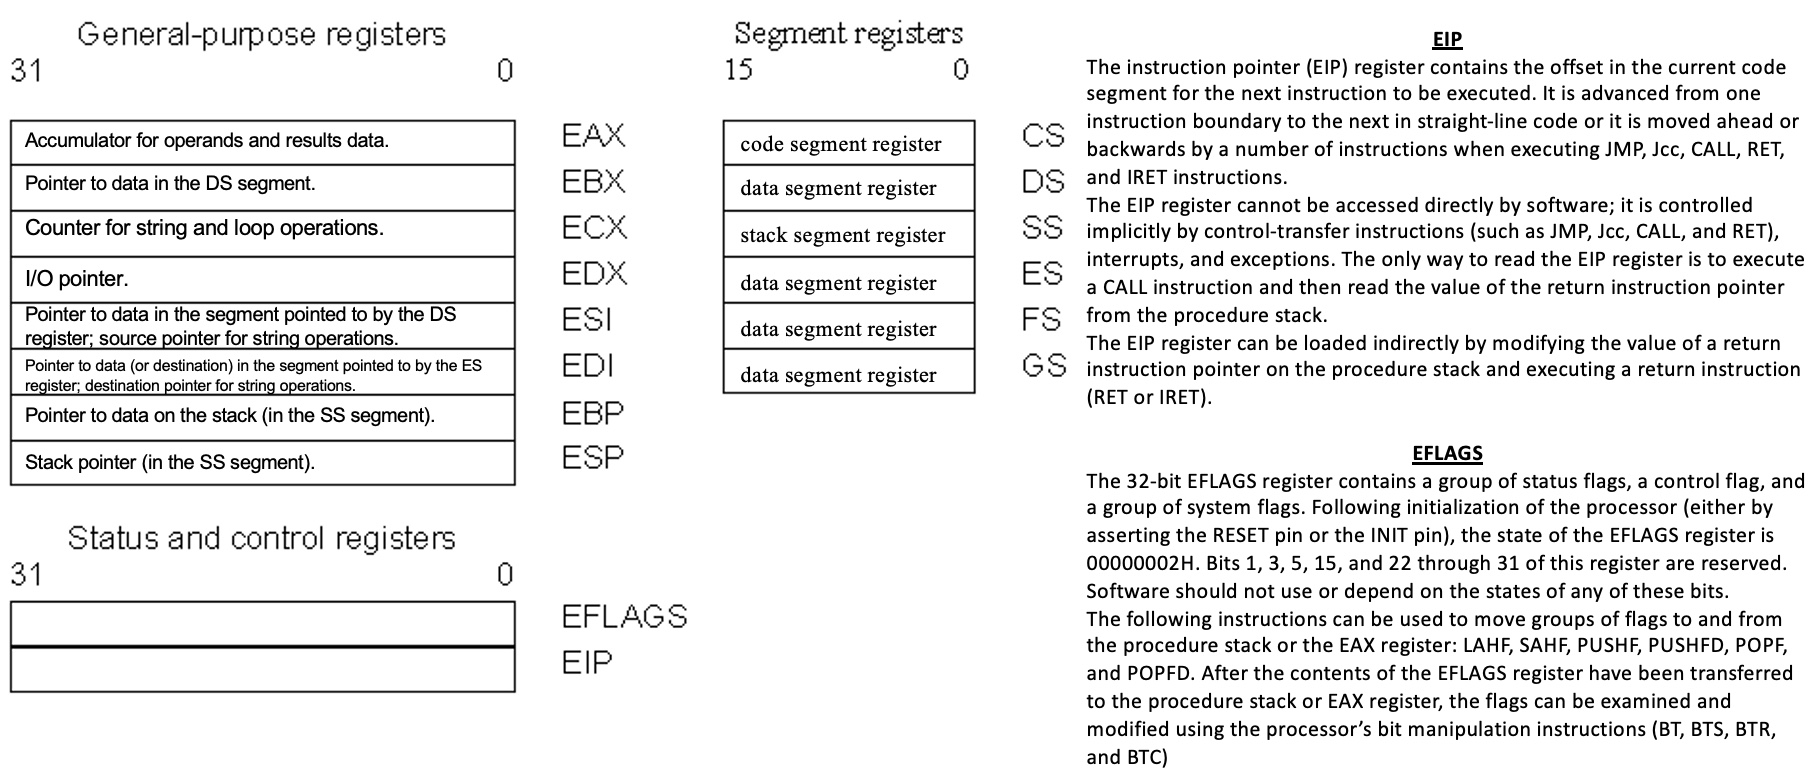
\includegraphics[scale=.27]{Register Diagram.jpeg}
\end{figure}

\subsubsection{The Stack}
The stack is one of two places that a value can be set aside. 
Registers are not managed by a processor and to use one you just need to load a value in it. 
Often there will not be registers available or there is a particular reason a variable will need to reside in RAM instead of in a register. 
That’s when you’d put a variable on the stack instead~\cite{Reversing}.

The stack is a short term storage space in memory that gets utilized by both the CPU and the program. 
It is the spot where short term information gets put when a register can not be used for whatever reason. 
Registers are for the shortest term data while the stack is for the second shortest. 
The stack lives in RAM like all other data and is just a carved out section for intermediate term data. 
Modern operating systems tend to manage multiple stacks at the same time. 
Each of the concurrently running stacks is a representation of a program or thread~\cite{MasteringRE}.

Stacks use Last In First Out data management. 
Items are pushed on the top of the stack and popped from the bottom of the stack. 
Memory in stacks is allocated from the top down where the first in address is allocated and used first while the stack grows backwards towards lower addresses~\cite{Reversing}.

\subsubsection{Flags}
One of the registers you may have noticed from the previous figure is the EFLAGS register. 
This is a collection of special IA-32 registers that contain system and status flags. 
The system flags’ job is to manage the different modes and states of the processor. 
The status flags are what a reverse engineer will typically be more interested in and are used by the processor to record its current logical state~\cite{Reversing}. 
They are often updated by various logical and integer instructions so they can record the outcome of these actions. 
There are also instructions whose operation conditions are dependent on the values for the status flags. 
This is what allows sequences of instructions to run different operations depending on what different input values may be, etc. 

Flags in IA-32 are the crux of conditional code. 
Arithmetic instructions check operand conditions and then set processor flag conditions based on the resulting values. 
There are also sets of instructions designed to read the flags and do different operations based on the value. 
An example of a popular instruction set is Jcc or the Conditional Jump. 
It tests for predefined flag values and then jump depending on whether or not it matches with the specified conditional code~\cite{intelManual}.

\subsubsection{Functions}
Instructions are the actual actions specified in assembly code. 
They are formatted with operation code (opcode) and one or two operands~\cite{Reversing} 
The opcode is what you are asking the computer to do such as MOV or JMP. 
The operand is the parameters that get passed to the opcode or the data being manipulated. 
Certain instructions will have no parameters. Data in assembly comes in three basic forms. 
There are register names, immediate data, and memory addresses. 
Register names are the names of the general purpose registers to be read from or written to like the EAX, EBX, etc. 
Immediate data is constant values that are embedded into the code and usually indicates there was a hard coded value in the source code. 
Memory addresses are the locations of operands stored in RAM. 
It can be hard coded and tell the processor where to read to and write from. 
It could also be a register with a value that will be used as a memory address. 
It is also possible to combine a register with an arithmetic operation and a constant so that there is some base address and then an index offset~\cite{Reversing}.

General purpose instructions are the ones that deal with program flow, logic, arithmetic, string operations, and basic data movement. 
They deal with data stored in memory at the general purpose registers, EFLAGS register, segment registers, and address information stored in memory ~\cite{Reversing}.

The MOV instruction shows up most frequently in most IA-32 instruction sets. 
This one deals with basic data movement. 
It takes in a destination operand and a source operand then moves the data from the source to the destination. 
The sources can be registers, immediate, or memory addresses. 
It is important to note that MOV cannot transfer data through memory, it can only take it out or put it in. 
The destination address can be a memory address (using a register or an immediate) or a register~\cite{Reversing}.




\section{Example Problems}
\subsection{Reversing Hello World}
Before taking on the larger endeavor of reversing a program written in a declarative language (SwiftUI), it’s important to start with the basics. 
Figure [insert figure here] shows a simple ‘Hello World’ program in C. 
To add some complexity, a few random variables and data structures were thrown in as Easter eggs. 
This is the program whose decompilation will be used as a jumping off point.
\begin{figure}[h]
\caption{Hello World Program}
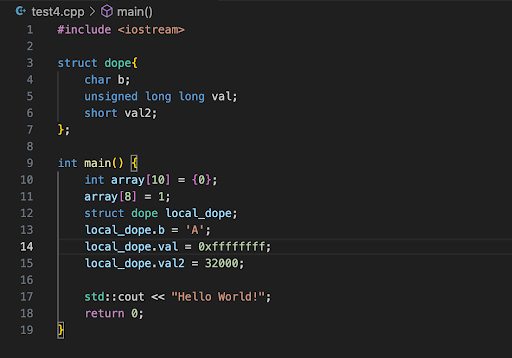
\includegraphics[scale=.75]{HelloWorldSource.png}
\end{figure}
Figure 3 is the decompilation of the program once it was put through Ghidra. 
The first thing to note is how with even a relatively low level language like C, the instructions in the code more than doubled. 
The disassembly being shown in the figure is also only a portion of Ghidra’s output. 
The figure only shows the function section of the program output when imports, exports, labels, classes, etc take up the large majority of the program. 
One important part of reverse engineering is sorting through all of the information to find out what exactly is important to the reverser. 
Some reverse engineers refer to this process as finding the shape and edges of the data. 
\begin{figure}[h]
\caption{Hello World Disassembly}
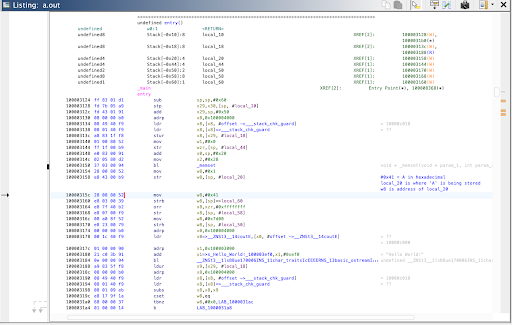
\includegraphics{HelloWorldGhidra.png}
\end{figure}
With the important section identified, it is time to analyze the assembly code.
One thing to keep in mind with the disassembled code is that all the values will be stored in hexadecimal. 
A good place to start is with the values we know will need to be stored. 
In the array there are 10 variables which all get set to 0, except for the eighth array member which is changed to equal 1. 
In our local\_dope struct there are three variables equal to ‘A’, ‘0xffffffff’, and 32000. 
The highlighted line in the figure shows ‘A’ being stored in the register w8. Shortly after, \#0xfffffff shows up without needing to be translated into hexadecimal. 
\#0x7d000 is the hex for 32000. 
This surface level analysis offers a glimpse into the methodology of more complex reverse engineering. 
Lastly, the 'Hello\_World!' gives us the final piece of information we need to know about what the program is.

\subsection{Crack Me}
The next step in practicing reverse engineering is trying a Crack Me problem. 
Crack Me problems are toy problems designed by other software developers to help reverser's practice their skills. 
Usually there’s an executable that opens up a little puzzle. 
The puzzles usually involve finding a password but can involve any number of things like decryption, key generation, etc. 
This section will cover the process of reverse engineering a simple crack me.

The first step I took in reversing this program was checking the header and libraries as shown in Figure 4 and 5.
\begin{figure}[h]
\caption{Crack Me Header}
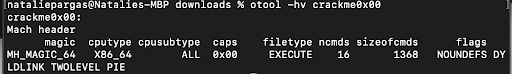
\includegraphics{crackmeheader.png}
\end{figure}
\begin{figure}[h]
\caption{Crack Me Libraries}
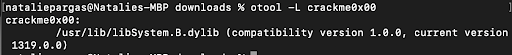
\includegraphics{crackmelibs.png}
\end{figure}
  
Both of these steps were done with an executable dumping tool called ‘otool’. 
The header information shows that the assembly language being used is x86. 
The library dump shows that the only library being linked is the system library. 
While these tools didn’t offer that much information about this particular program, they are very useful in programs that have more dependencies and more specific assembly languages. 
These dumping tools ended up being vital later in the project because they offered insight into what libraries were being linked from the project's declarative language as well as what assembly language was being used with Apple’s modified version of ARM64. 
Next, otool was used once again to list the strings. 
This is a vital part of reverse engineering and is useful to be able to refer back to during the process. 
Figure 6 shows the result of the string dump.

\begin{figure}[h]
\caption{Crack Me Strings}
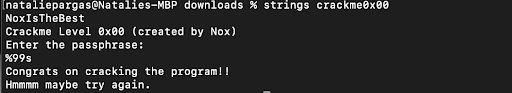
\includegraphics{crackmestrings.png}
\end{figure}
  
Examining this more closely, you can see that there’s only a few strings that give a very clear idea of what the program is designed to do. 
There’s a random string, the title of the program, a passphrase prompt, a string indicating the expected input, a congratulations message, and an incorrect guess message. 
With just this information, you could easily make an educated guess on what the password is. 
Most likely the passphrase will be the one random string that doesn’t get given easily in the executable. 
But for the sake of gaining understanding of the process, it’s good to go over the decompiled code. 
Figure 7 shows the decompiled code.
  
\begin{figure}[h]
\caption{Crack Me Ghidra Disassembly}
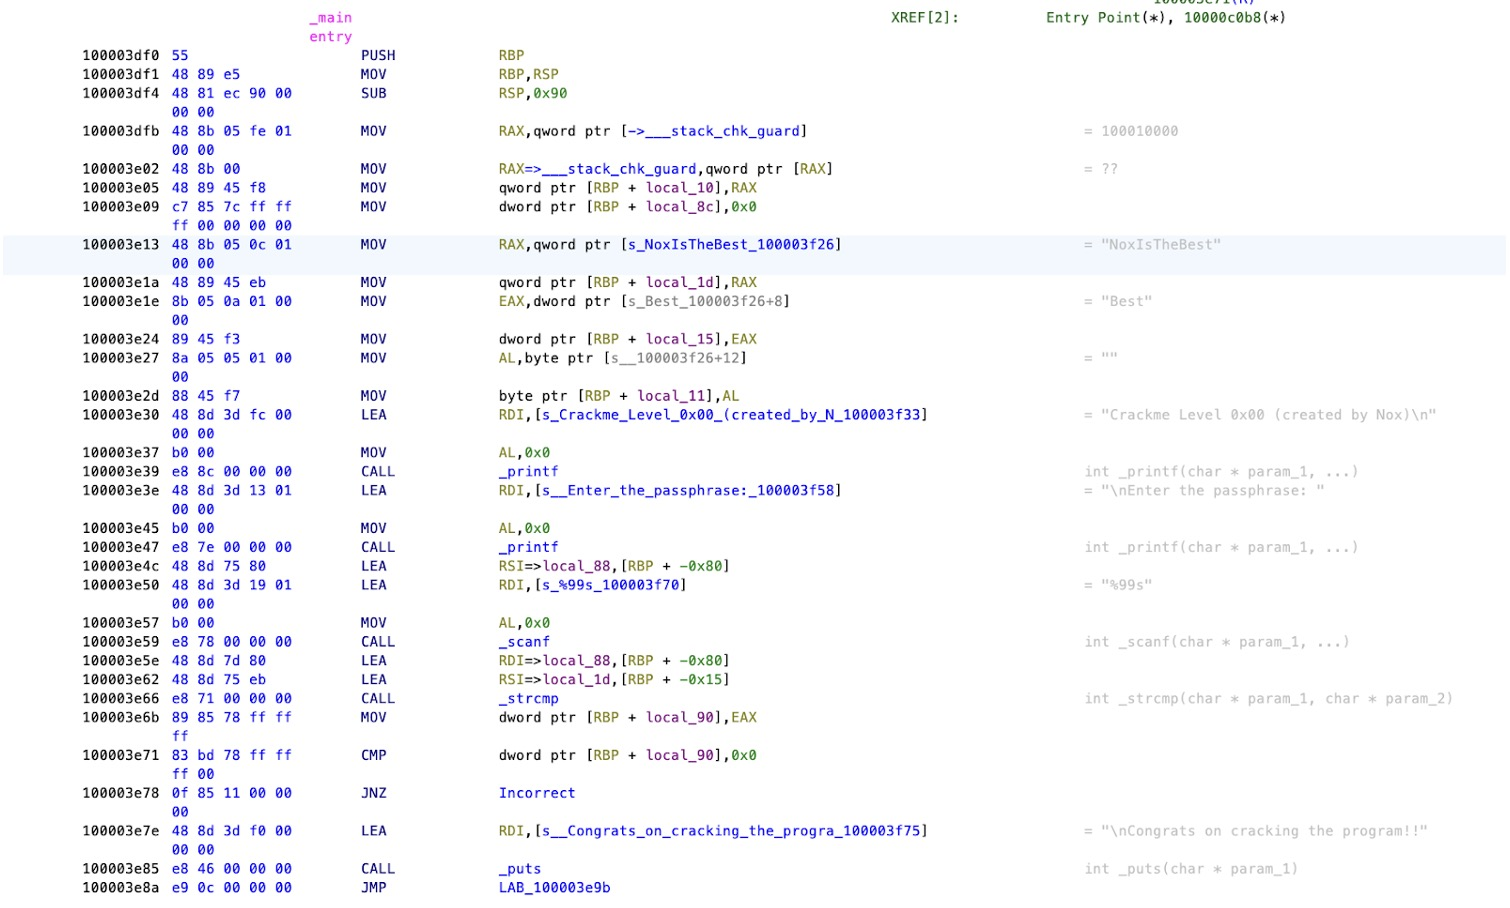
\includegraphics{crackmeghidra.png}
\end{figure}
  
The first thing to do is find the entrance into the program. 
Ghidra already labeled the ‘\_main’ at the top but the strings and function calls reaffirm this as the right section to be looking over. 
Next, thinking back to the string dump, it’s likely that the password will be near whatever function takes input. 
Prior knowledge of programming informs the reverser that after getting the user input, the input string will need to be compared to the right answer. 
Thankfully Ghidra was able to identify the function ‘scanf’.
  
\begin{figure}[h]
\caption{Crack Me Code Section 1}
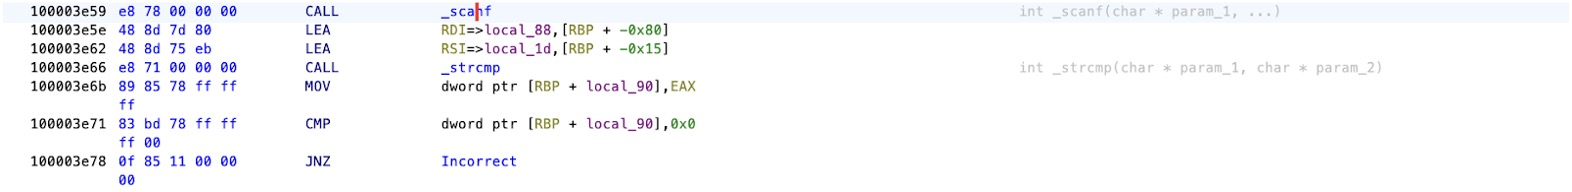
\includegraphics{crackmescanf.png}
\end{figure}
  
Inspecting the code section at figure 8, it shows that the variable local\_88 contains the user input. 
This is because it loads a \%99s into the RDI register to prepare for the input directly above where scanf is called. 
RSI has local\_1d loaded into it and that variable is immediately ‘strcmp’ compared to local\_88. Using these clues, one could infer that local\_1d contains the password. 
To verify, a reverser should always retrace and check.
  
\begin{figure}[h]
\caption{Crack Me Code Section 2}
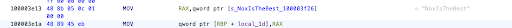
\includegraphics{crackmeRAX.png}
\end{figure}
  
The first instance of local\_1d contains the register RAX 9. 
RAX has the qword ptr ‘ s\_NoxIsTheBest\_100003f26’ moved into it right above. 
s\_NoxIsTheBest\_100003f25 only contains the string “NoxIsTheBest”. 
That string is probably the password, but all that’s left is to check. 
Figure 10 shows the result.
\clearpage
\begin{figure}[h!]
\caption{Crack Me Code Executable}
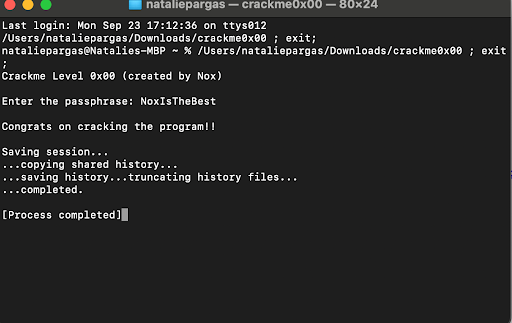
\includegraphics[]{crackmeexe.png}
\end{figure}
The attempt was a success and the crack me was successfully reverse engineered!
  

\section{Java RE}
\subsection{JVM}
\subsection{Reversing Bytecode}
\subsection{Java Name Obfuscation}
\subsubsection{Obfuscating names for .class file}

\section{Mobile RE}
\subsection{Hybrid Approach}
\subsection{Symbolic Execution}
\subsection{Generating UML Diagram}
\subsection{Android}
\subsubsection{Tools}
\paragraph{Dalvik VM Android}
\paragraph{APK Tools}
\subsection{Apple?}
\subsubsection{Obj C tools}




 


%!TEX root = ../main.tex
\chapter{Methods}\label{bibind}
\section{Test 1: Altering the app}
To ensure that I would be able to successfully complete this project, I first needed to confirm that I could alter the app’s behavior in some meaningful way. At the time, the only tools I had available were my MacBook with Android Studio installed. I was running the app on an emulated Android device and quickly found out that in order to use Frida—the dynamic instrumentation toolkit I planned to rely on—I needed to root the emulator. While I had decompiled parts of the app using Jadx, modifying the code that way wasn’t practical. Decompiled code generally can’t be recompiled cleanly, and reconstructing the original logic is both difficult and time-consuming.
Given that Frida was going to be the foundation of my approach for real modifications later on, it made the most sense to start testing with it from the beginning. While it’s true that .xapk files for this app weren’t obfuscated and could have been manually edited and re-signed, that path would have diverged from the strategy I’d ultimately use. Instead, I committed to building out a working Frida workflow right away.
The first step was gathering all necessary tools. This included Frida itself, the frida-server binary compiled for android-arm64 (version 16.7.14), and Objection, a utility built on top of Frida for runtime mobile app exploration. I also installed the Android command line tools directly from Google’s site, which are separate from Android Studio’s full IDE.
With those in place, I turned to setting up a rooted Android emulator. I used rootAVD, a script that modifies emulators to grant root access. Since I was working on an ARM64 Mac, I selected version 12 (Android S) from rootAVD’s compatibility chart. Using Android Studio, I downloaded the system image for API level 28 with an ARM64 architecture. After confirming the image was downloaded, I launched the emulator from the terminal using the emulator command. I first listed the available virtual devices, then ran the appropriate command to launch the desired AVD.
Inside the rootAVD directory, I ran the script by typing ./rootAVD.sh. I listed all the AVDs and selected the correct ramdisk.img from the path system-images/android-28/default/arm64-v8a. If everything was patched successfully, the emulator would shut down and then boot up again normally. A grey or black screen during boot was a sign that something had gone wrong. Once the emulator was running again, I verified root access using ADB. I ran adb shell, then typed su, followed by whoami. If the output returned "root," that meant the emulator was successfully rooted.
At that point, I was ready to run Objection. I launched it in a new terminal window by attaching it to the app’s process using the command objection -g com.loreal.ysl.perso.lips explore. If everything was working correctly, Objection would connect to the app, allowing for runtime exploration and testing.
Next, I needed to get frida-server running on the device. I navigated to the folder where the binary was located and made it executable with chmod +x. Then I pushed it to the emulator’s file system using ADB. Specifically, I placed it in /data/local/tmp using the command adb push frida-server-16.7.14-android-arm64 /data/local/tmp/frida-server. After entering the device shell and switching to root again with su, I launched the server in the background using ./frida-server &. A successful start would return a process ID.
With the Frida server running and everything hooked up, I tested a simple proof-of-concept string replacement. I began by choosing the string I wanted to replace: “No activities yet.” To work with it at the memory level, I converted the string to hexadecimal using echo -n "No activities yet" | xxd -p, which gave me the raw hex representation of the text. I then used Frida’s memory search capabilities to locate that hex sequence in the app’s memory.
Next, I decided on the replacement string—“Natalie activities”—and repeated the process to convert it to hex using the same xxd command. Then I retrieved the process ID (PID) of the running app using adb shell pidof com.loreal.ysl.perso.lips. With that PID, I ran the Frida script I had written to replace the original string with the new one. The command was frida -U -p <PID> -l replace_textview.js. Occasionally, Frida throws unhelpful syntax errors—like missing semicolons—that don’t actually affect runtime behavior. Even if such an error appeared, I would go back to the app, let it load, and check if the text had been replaced. And in this case, once the relevant screen rendered, the string had indeed been swapped out, confirming that the setup was working.



\section{Environment Setup (components)}
\subsection{Rooting the phone}
Rooting the OnePlus 8T was a necessary step for me in the broader context of reverse engineering a mobile application. I had several reasons for wanting to root the device, all of which stemmed from the technical demands of the project I’m working on.
The first and most pressing reason is that rooting is essential for hooking into the app's internal processes. Through my early experimentation, I discovered that modifying the app’s behavior would require a Man-In-The-Middle (MITM) attack, and tools commonly used for this—such as Frida—typically require root access to function properly.
Additionally, rooting a device grants access to lower-level Bluetooth packet data, which is crucial for my analysis. On a rooted phone, I can use Frida scripts to log system-level Bluetooth reads and writes that would otherwise be inaccessible. If progress slows using the current toolset, more advanced offensive techniques, such as those available through Kali NetHunter or Ubertooth, may become necessary. These tools also work more effectively on a rooted device.
Rooting a phone, however, wipes all data stored on it. For this reason, any data I intend to keep must be backed up and restored after rooting is complete. Overall, reverse engineering is an inherently unpredictable process, and having access to a wide range of tools—many of which require root access—means I can pivot more quickly if one approach hits a dead end.

Step 1: Downgrade to Android 11
The first hurdle in rooting the device was downgrading the operating system. Although I found a guide for rooting the phone on Android 14 (the version it shipped with), it required a specific boot image that I couldn’t locate. My phone’s variant, the OnePlus 8T KB2005 (global version), receives incremental boot image updates, which means a complete boot image for patching and reuploading isn't publicly available.
I attempted to use a boot image I found online, but it didn’t match my Android version, which resulted in the phone becoming soft-bricked. To resolve this and simplify the patching process, I used the MSM Download Tool to downgrade the device to Android 11. I followed this XDA Developers guide: XDA MSM Tool Guide.
After connecting the phone to my PC via a trusted USB port, I had to troubleshoot some driver issues. Interestingly, the front USB ports on my PC didn’t recognize the phone reliably, while the back ports—connected directly to the motherboard—worked better. When the device appeared as QHUSB_BULK, I knew the Qualcomm USB drivers were improperly installed. I downloaded the correct drivers from Microsoft’s catalog: Qualcomm USB Drivers.
Next, I confirmed my build version: kb2005_14.0.0.602(EX01), indicating I had the International model, which uses the KB05AA firmware. I downloaded the corresponding MSM tool and followed these steps:
Launch MsmDownloadTool V4.0.exe.


At the login screen, choose "Other" and click "Next."


Select the correct target region (O2 for Global).


Press "Start" to initiate the flashing process.


Power off the device and allow it to cool.


Enter EDL (Emergency Download) mode by holding both volume buttons and plugging the phone into the computer.


Wait for the flash to complete (~300 seconds).
Step 2: Root the Phone
With the phone successfully downgraded, I proceeded to root it using another guide from XDA. I began by re-enabling Developer Mode, which involved tapping the build number eight times in the settings. Once Developer Mode was active, I enabled USB Debugging and plugged the device back into my computer. To ensure everything was working properly, I ran adb devices and fastboot devices to confirm the device was being recognized. If drivers weren’t functioning correctly, I had to reinstall them.
Next, I needed to identify which slot the device was currently using. I did this with the command fastboot getvar all, which showed that the current slot was a. With that information, I moved forward with extracting the boot image from the active partition. I used a semi-broken TWRP recovery image that I booted into temporarily with fastboot boot recovery.img. This version of TWRP doesn’t include a GUI but provides ADB shell access, which was all I needed. Inside the shell, I used the dd command to copy the boot_a partition to the SD card. After exiting the shell, I pulled the boot_a.img file from the device using ADB and then rebooted the phone normally.
Once I had the boot_a.img file on my computer, I transferred it to the phone’s internal storage, placing it in an accessible location like the Downloads folder. I then installed the latest version of the Magisk Canary APK on the phone. Opening the app, I selected the install option and chose "Select and Patch a File," pointing Magisk to the boot_a.img I had extracted earlier. This generated a patched image file named magisk_patched_a.img, which I copied back to my computer.
To proceed with rooting, I rebooted the phone into fastboot mode using adb reboot bootloader. Instead of flashing the patched image, I temporarily booted into it using the command fastboot boot magisk_patched_a.img. This gave me temporary root access. With the device booted into this patched environment, I opened Magisk again and selected the install option, this time choosing "Direct Install (Recommended)" to apply root access permanently to the internal boot image.
After the installation completed, I rebooted the phone and used a root checker app to verify that root access was working. Everything checked out, and the device was successfully rooted.


\subsection{Virtual Machine}
\subsection{Tools}
\subsubsection{JADX}
\subsubsection{Ghidra}
\subsubsection{APK Tools}
\subsubsection{JBSE (symbolic Java VM)}
\subsubsection{UML Diagram Creator (Ask Dr.Guarnera)}
\subsubsection{Emulator ?}

\section{Scripting}
\section{App Interoperability}



%%!TEX root = ../main.tex
\chapter{Methods}
Reverse engineering is a complex process with no universal solution. It often involves extensive trial and error, making it important to adopt a strategy that encourages rapid iteration while minimizing risk. In this case, the most practical approach was to prioritize simplicity and accessibility. The Android version of the app was selected for analysis, as it uses Java and Kotlin—languages that are generally more amenable to reverse engineering. Additionally, a man-in-the-middle (MITM) technique was chosen to intercept and manipulate data exchanged between the app and the target device.

The initial step involved verifying the ability to interact with the app by modifying data in a detectable way. Once this was confirmed, the next objective was to capture the data being transmitted between the app and the makeup printing device, along with identifying the method of transmission. The final step was to replicate that communication in order to send custom data to the device in the expected format.

\section{Decoding app data}
When trying to understand the communications between the app and the makeup printer device, one method that’s certifiably free of interpretation error is capturing the packet data sent over the air between the devices. Understanding the raw packets is also helpful if the app itself is too difficult to reverse engineer, as it enables direct interaction with the device and bypasses the app altogether. This is a common reverse engineering method because developers seldom bother to obfuscate Bluetooth packet data. Ultimately, the relevant data has to appear somewhere in the Bluetooth packets, it’s just a matter of decoding where and how it does.

\subsection{Testing with the nRF Connect App}
There are a few different ways to capture this packet data. As mentioned previously, one method is using a Bluetooth packet sniffer along with the nRF Connect app and Wireshark. This was my first test. The following figures show the device information I discovered using the nRF Connect app. It was fascinating to see how much information was accessible through nRF Connect alone. For example, Figure \ref{fig:nrfconnect3} shows the NUS\_ID, NUS\_RX, and NUS\_TX identifiers, which I previously found in Jadx after a long period of searching. The nRF Connect app revealed this information immediately, without even needing to connect to the device.


\begin{figure}[H]
	\centering
	
	\begin{minipage}{0.32\textwidth}
		\centering
		\includegraphics[width=\linewidth]{../Downloads/nrfconnect1}
		\caption*{}
		\label{fig:nrfconnect1}
	\end{minipage}
	\hfill
	\begin{minipage}{0.32\textwidth}
		\centering
		\includegraphics[width=\linewidth]{../Downloads/nrfconnect2}
		\caption*{}
		\label{fig:nrfconnect2}
	\end{minipage}
	\hfill
	\begin{minipage}{0.32\textwidth}
		\centering
		\includegraphics[width=\linewidth]{../Downloads/nrfconnect3}
		\caption*{}
		\label{fig:nrfconnect3}
	\end{minipage}
	
	\caption{NRF Connect screenshots}
	\label{fig:nrfconnect_all}
\end{figure}

% TODO: \usepackage{graphicx} required
\begin{figure}[H]
	\centering
	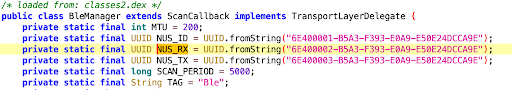
\includegraphics[scale=.8]{bleuuidjadx}
	\caption{}
	\label{fig:bleuuidjadx}
\end{figure}
Unfortunately, while this information was helpful, I wasn’t able to gather much more from nRF Connect because the device would connect and then disconnect shortly afterward. Even so, this discovery was valuable because it suggests that a handshake occurs between the app and device after connecting, which the nRF Connect app does not perform.

Without dumping the firmware, I cannot know exactly what occurs during this handshake. However, I can begin piecing it together by examining the onConnectionStateChanged() function in Jadx. Figure \ref*{fig:statemachineonconnection} presents a model of this function. It illustrates how the function checks Android’s BluetoothProfiles to determine whether the constant indicates a disconnected state (0) or a connected state (2). If connected, the function proceeds to request an MTU of 200 from the device. This is likely the point at which issues arise, as the app’s custom MTU is significantly larger than the general Bluetooth MTU used by the nRF Connect app.

% TODO: \usepackage{graphicx} required
\begin{figure}[H]
	\centering
	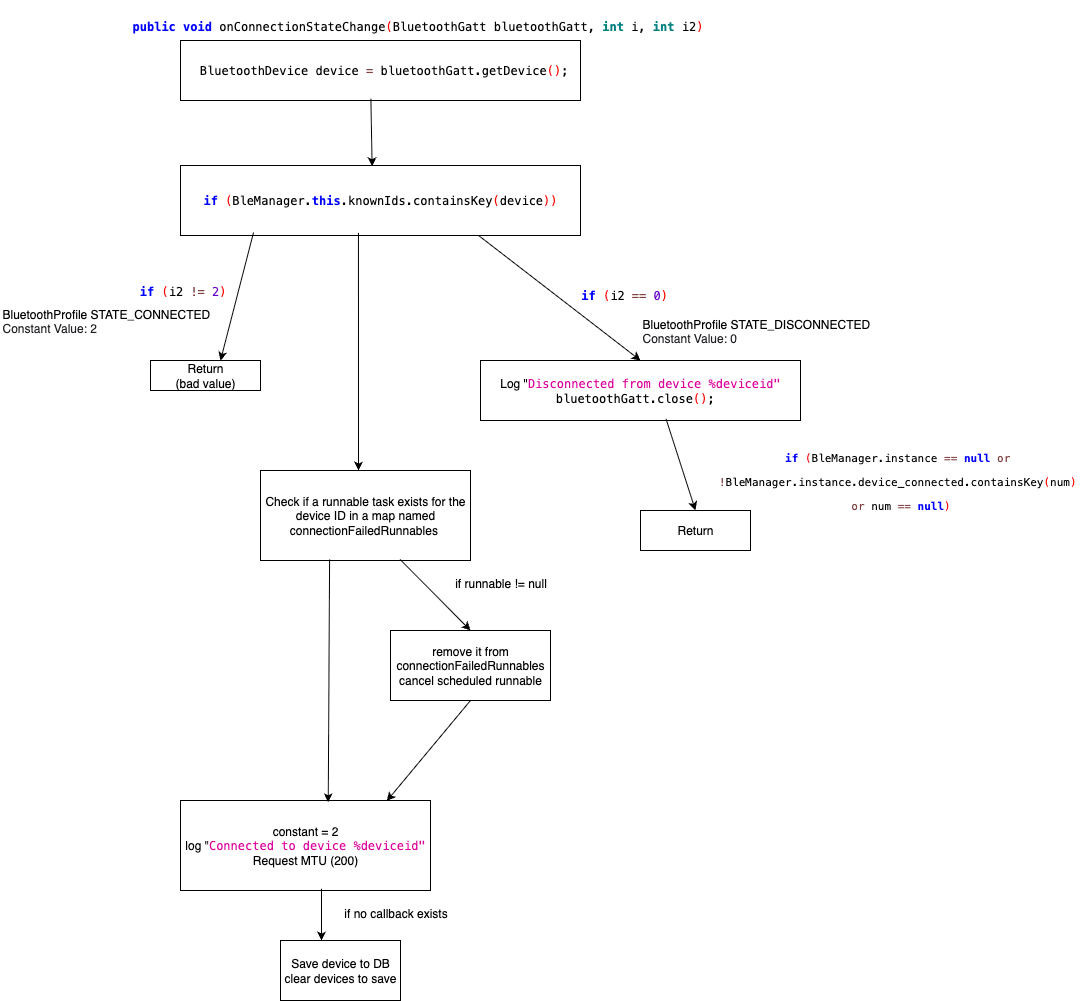
\includegraphics[scale=.5]{statemachineonconnection}
	\caption{}
	\label{fig:statemachineonconnection}
\end{figure}

Nevertheless, if the device had remained connected, it would have been possible to conduct tests and observe the raw byte payloads along with the characteristics transmitting them. For certain devices, it is even feasible to reverse engineer them using only the nRF Connect app, which is both impressive and somewhat concerning.

This example represents my first test that did not fully succeed. Moving forward, there will be many more attempts that end in a similar manner, where progress is made but the puzzle remains incomplete. In reverse engineering, flexibility and patience are essential. Because each piece of software and hardware differs, methods effective in one case may fail in another. Many projects are ultimately abandoned due to time constraints rather than technical impossibility.

\subsection{Update on the nRF App}
After writing the previous section, I was able to access the device through the nRF Connect app by switching to Android. I had the nRF Connect app running when I opened the YSL app and connected to the device, which triggered a popup on my phone indicating that an “unknown device was detected” and asking whether I wanted to connect for debugging. 

When I reopened the nRF Connect app, the device and all of its packet information became visible. However, when I returned to the YSL app, the device appeared as disconnected and required me to disconnect it in the nRF Connect app before I could reestablish connectivity.
I was able to run several tests and capture definitive live packet data. During these tests, the nRF Connect app attempted to translate the packet data into Unicode strings. This translation revealed that the shade information is transmitted by the device in one of the initial packets, regardless of whether a dispense occurs or a color is selected.
% TODO: \usepackage{graphicx} required
\begin{figure}[H]
	\centering
	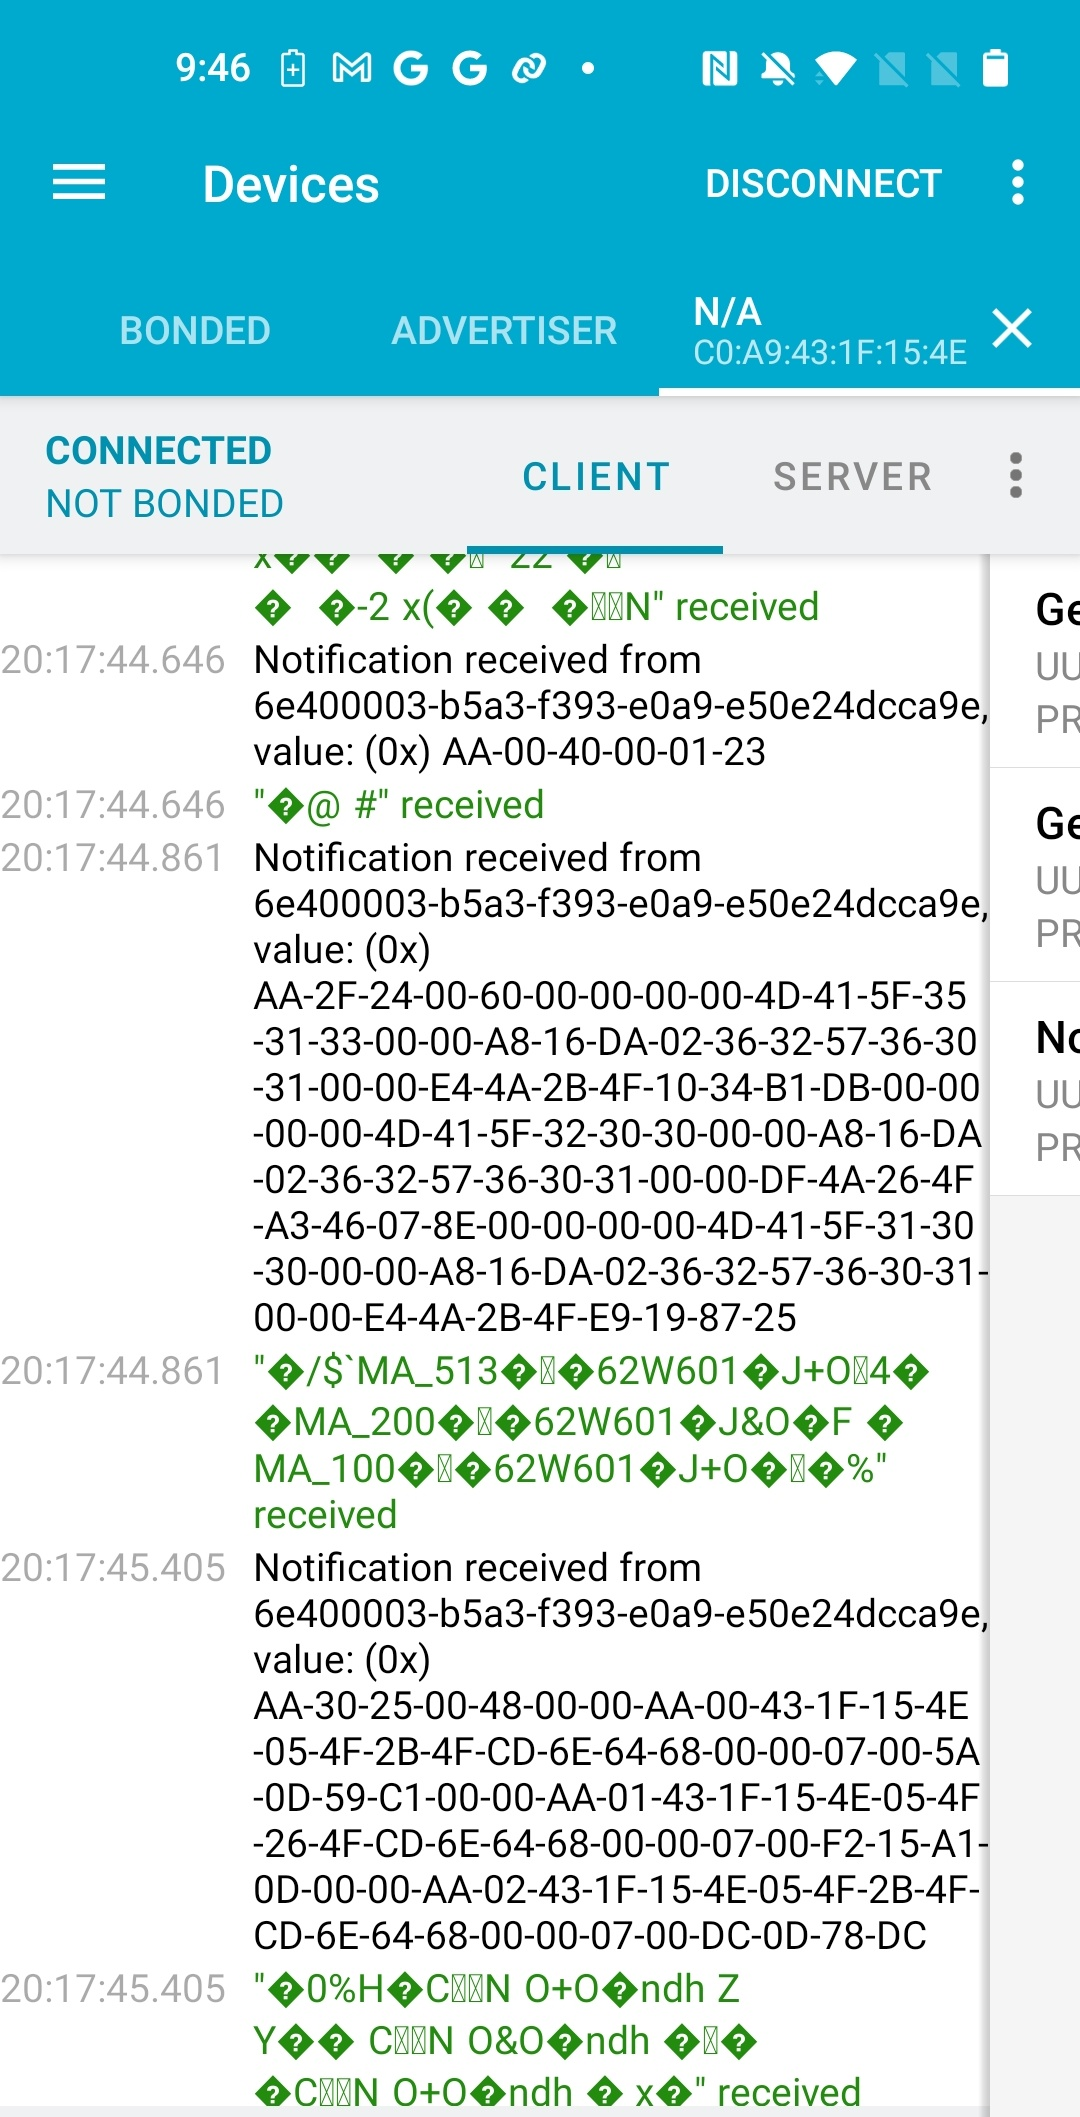
\includegraphics[scale=.15]{nrf_connect_android}
	\caption{}
	\label{fig:nrfconnectandroid}
\end{figure}

\section{Testing with the nRF Sniffer and Wireshark}

Because the nRF Connect app could not interface with the device, it became essential to use a Bluetooth sniffer. When selecting a sniffer, I had to weigh the overall cost of setting up the environment, which led me to choose the nRF52840 Dongle. My research indicated that this dongle was reliable and offered significant value for its modest \$10 cost. Additionally, it is manufactured by the same company that appeared to provide the software development kit used by the target device. Although more advanced and expensive sniffers can yield more detailed results, I recommend that anyone beginning this process start with a reasonably priced sniffer and consider investing in a higher-end tool only if the initial setup proves insufficient.

Setting up the nRF52840 Dongle required several steps. The dongle itself is simply a piece of hardware that serves no specific function until the appropriate software is flashed onto it. The first step involved installing the nRF Util tool, which depends on the presence of the SEGGER J-Link software. If this software is missing, outdated, or incorrectly configured in the system path, the flashing process will not work properly. The next requirement was to install the ble-sniffer command. Completing these installations prepared the environment for flashing the dongle.

The subsequent step involved locating the directory where nRF Util was installed. Within this directory, the corresponding firmware for the sniffer could be found, usually named in the format sniffer\_nrf52840dongle\_nrf52840\_*.zip. After connecting the dongle to my computer—I use a MacBook equipped only with USB-C ports, though a USB adapter functioned without issue—I proceeded to install the nRF Util device command using nrfutil install device. Running the command nrfutil device list allowed me to identify the correct device. Once detected, I programmed the dongle by executing nrfutil device program --serial-number <serial-number> --firmware <file>, substituting the serial number identified earlier and the appropriate firmware file. At this stage, the dongle was flashed and ready for use.

Following these steps, I was able to begin sniffing Bluetooth traffic immediately. When the dongle successfully captured packets, an LED light on the device would blink with each sniffed packet. The setup functioned perfectly on the first day. However, during retesting the following day, the LED stopped blinking, and the dongle was not recognized correctly. Diagnosing the problem required extensive troubleshooting. Sometimes, the dongle appeared in the nRF Connect app, while at other times it disappeared entirely and was not visible from the command line. Ultimately, I had to wipe the dongle and repeat the flashing process, which seemed to restore its functionality.

Nevertheless, I encountered a significant issue: the dongle worked a bit too well. I was testing in a densely populated apartment complex where numerous Bluetooth devices were active, as previously observed through the nRF Connect app. The dongle’s LED blinked incessantly, making it impossible to isolate packets relevant only to my target device and specific tests. Figure \ref*{fig:wiresharkpacketsniffing} illustrates a log in which the dongle captured over 32,400 packets.

% TODO: \usepackage{graphicx} required
\begin{figure}
	\centering
	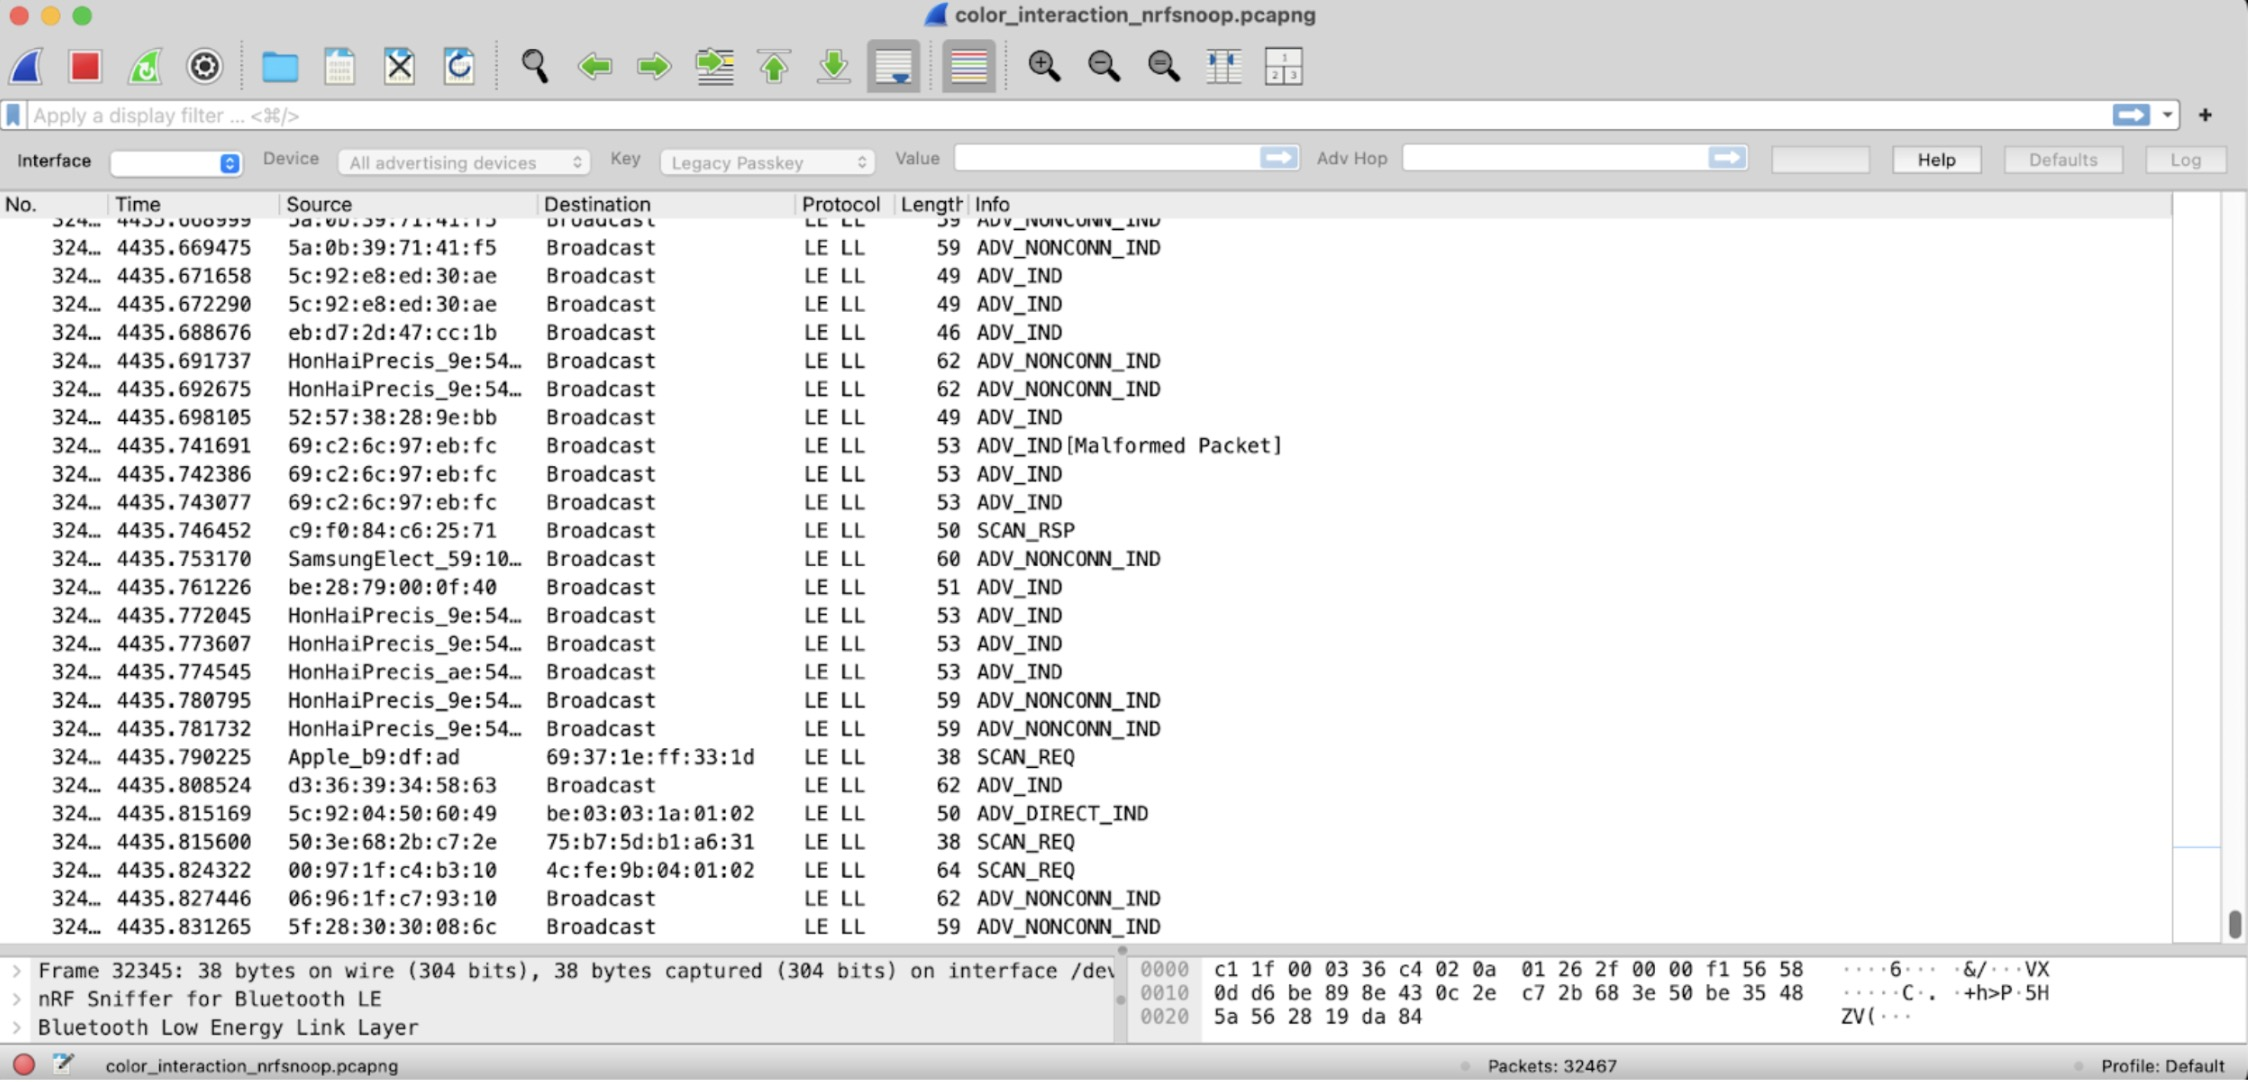
\includegraphics[width=0.7\linewidth]{wireshark_packet_sniffing}
	\caption{}
	\label{fig:wiresharkpacketsniffing}
\end{figure}

Although Wireshark provides powerful commands for filtering captured data, there was insufficient information to determine suitable filters for isolating the target packets. Attempts to filter based on segments of UUIDs yielded no matches, and manually parsing such a large volume of data was impractical. Fortunately, with an Android device, it is possible to extract HCI snoop logs, which record all of the phone’s Bluetooth interactions. To reduce the volume of data and improve the chances of identifying relevant packets, the next step was to pull these logs directly from the phone.

\section{Analyzing the HCI Snoop Logs}
The first step in obtaining Bluetooth HCI snoop logs is to enable Bluetooth debugging on the device. This requires ensuring that USB debugging is already activated, which should be the case given the extensive ADB debugging performed on the phone thus far. Once confirmed, navigate to the developer settings and enable the option labeled “Enable Bluetooth HCI snoop log.”

With logging enabled, it is then necessary to generate traffic to capture in the log. For my initial test, I chose to record a connection event between the application and the makeup printer device.

Retrieving the log from the device proved somewhat more complicated than anticipated, as the file was not stored in the expected location. To locate it, I ran the following command:
find /data -iname '*btsnoop*'

This is a prudent step to avoid attempting to pull the log from an incorrect path. Ultimately, the btsnoop log was located in the directory:

/data/misc/bluedroid

Bluedroid is Android’s Bluetooth stack, and files stored in its directories are inaccessible to non-root users due to the system’s permissions model. To retrieve the log, I first copied it to the device’s SD card using the command:

cp /data/misc/bluedroid/2025\_05\_28\_14\_24\_03\_btsnoop.txt  /sdcard/btsnoop\_hci.log

I then verified the file’s presence on the SD card by executing:

ls -l /sdcard/btsnoop\_hci.log

Once confirmed, I used the adb pull command to transfer the log to my Mac for further analysis.

With the log successfully copied to the computer, it became ready for examination in Wireshark. To contextualize the data, it is useful to recall the role of Bluetooth’s Host Controller Interface (HCI), which defines the standard communication protocol between the higher-level host and the lower-level controller. Generally, these logs are text files that capture HCI commands, events, and data packets. As a brief reminder, HCI commands are instructions sent from the host to the Bluetooth controller (for example, a disconnect command), while 

HCI events are the corresponding responses sent from the controller back to the host (for example, a disconnection complete event). Each entry in the log represents a specific communication action or response.

% TODO: \usepackage{graphicx} required
\begin{figure}
	\centering
	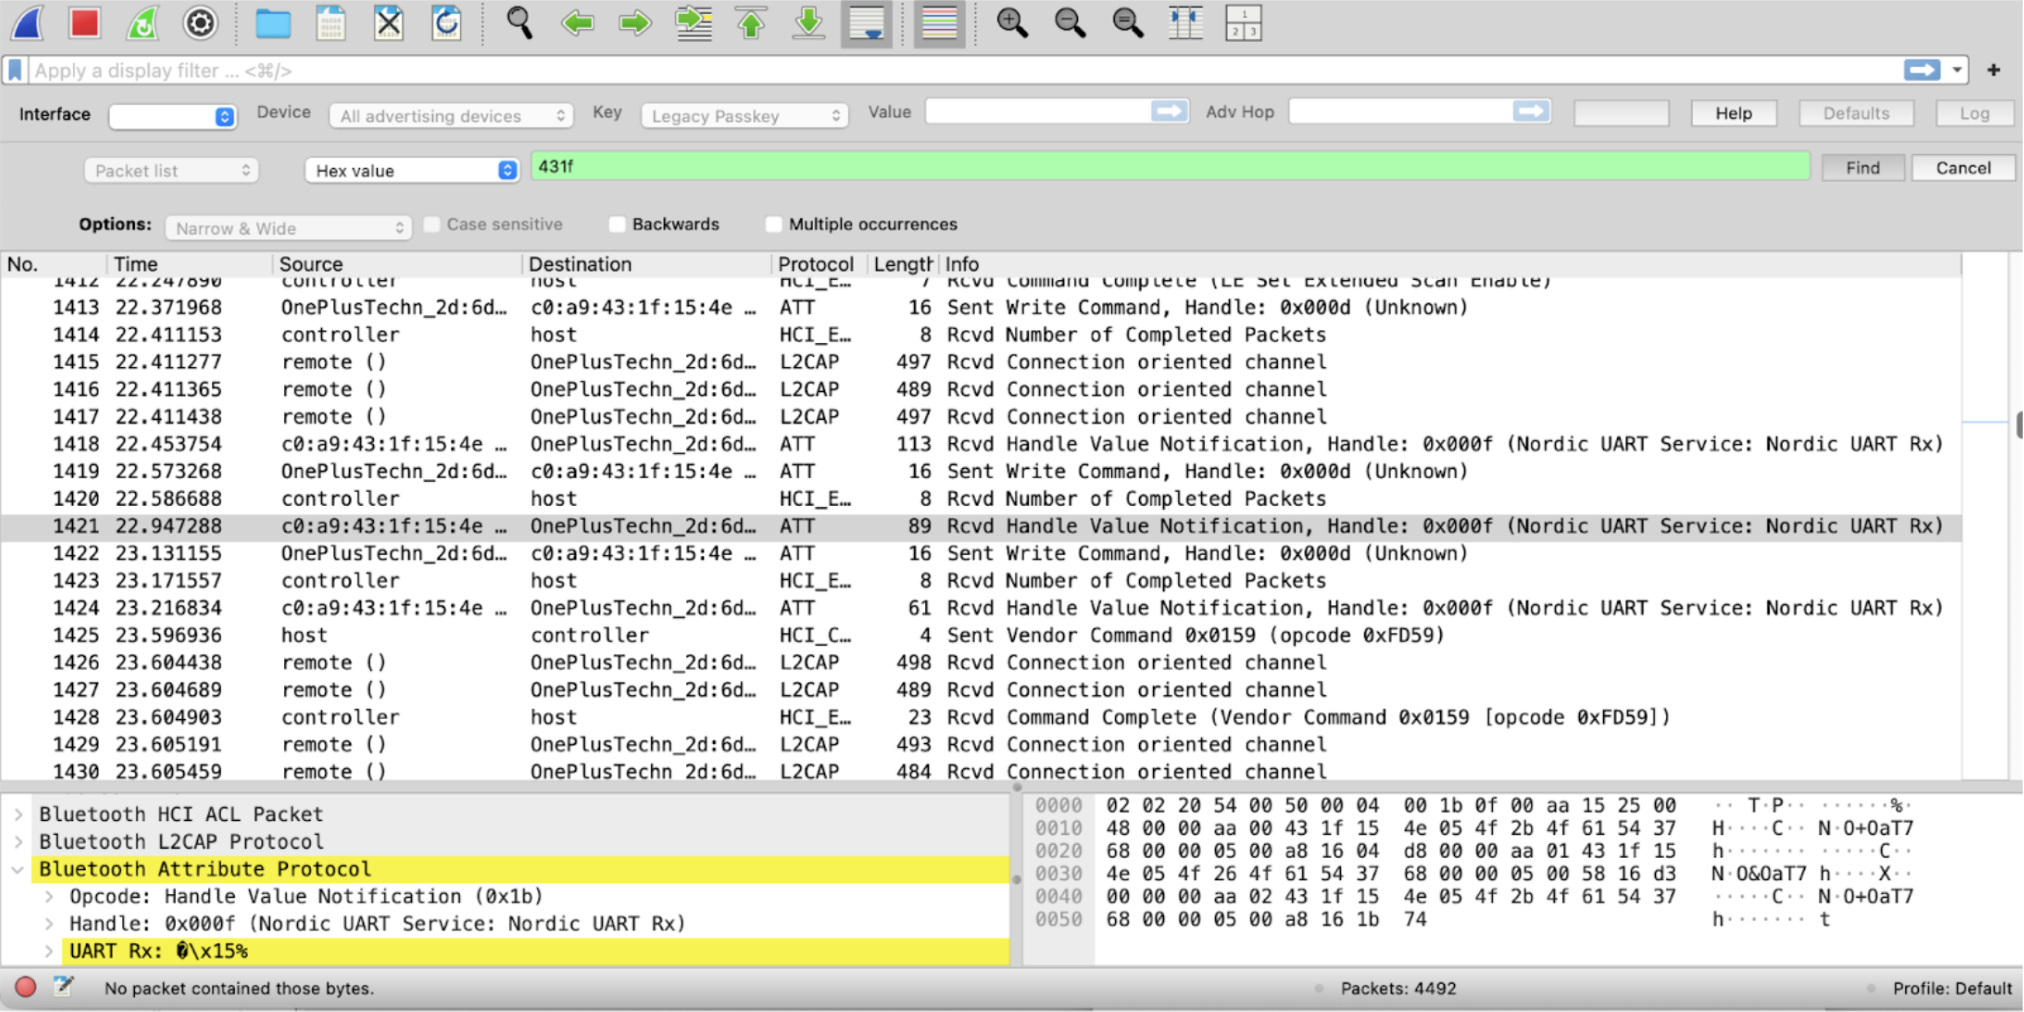
\includegraphics[width=0.7\linewidth]{hci_snoop_log}
	\caption{}
	\label{fig:hcisnooplog}
\end{figure}

Despite filtering the capture to a specific event, the log still contained a substantial number of packets (4,482 in total). To simplify analysis, it is advantageous to use filters within Wireshark. One useful filter for this scenario is the btatt filter, which allows the user to isolate only the Attribute Protocol (ATT) traffic. This protocol governs the discovery, reading, and writing of attributes between a client and a server device.

By narrowing the captured data using this filter, it becomes significantly easier to identify relevant packets that represent interactions between the phone and the device. For instance, in Wireshark I identified communication from the phone, OnePlusTechn\_2d:6d:b6, directed to the device c0:a9:43:1f:15:4e, in which the phone issued a write command.

% TODO: \usepackage{graphicx} required
\begin{figure}
	\centering
	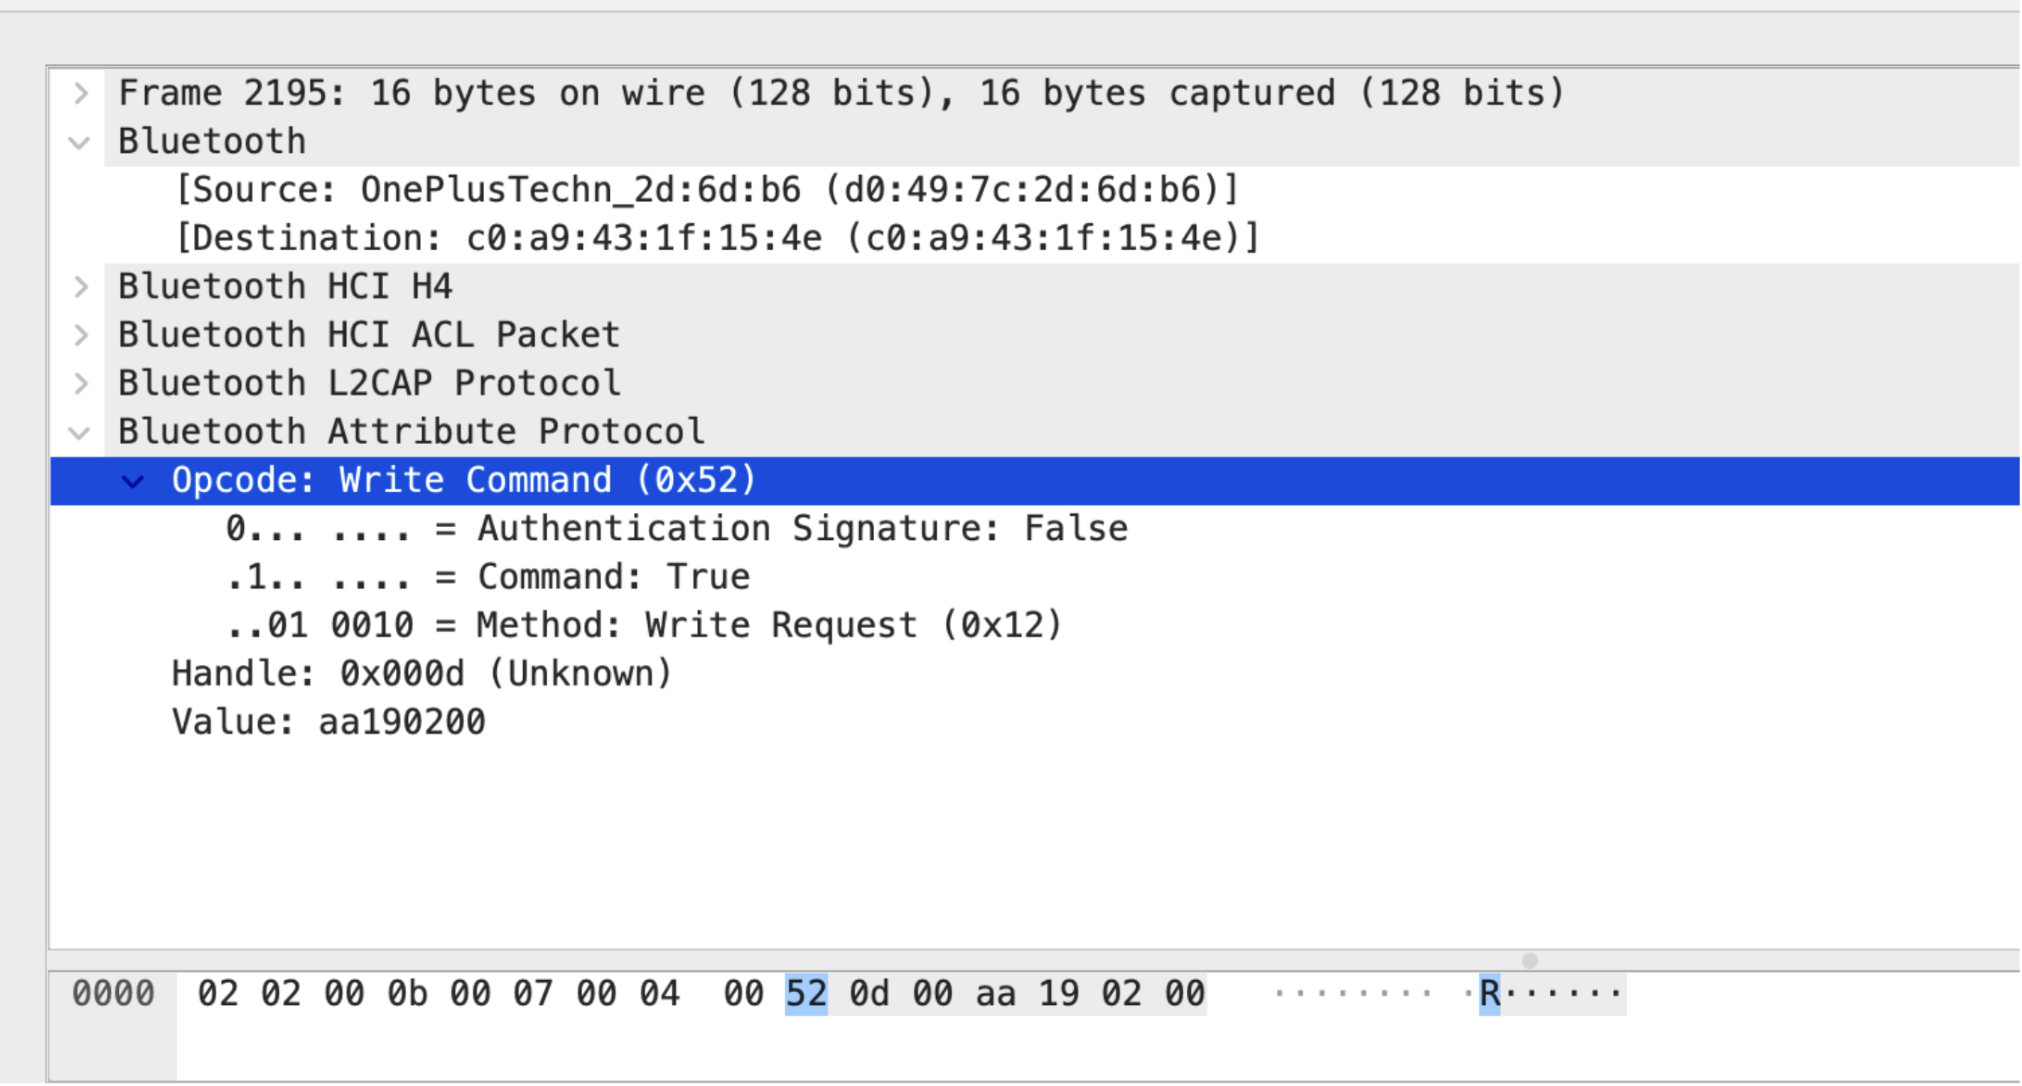
\includegraphics[width=0.7\linewidth]{hci_tree_wireshark}
	\caption{}
	\label{fig:hcitreewireshark}
\end{figure}

By examining the attribute tree in Wireshark, it is possible to locate both the handle and the value of this write operation. In this case, the write occurred to the characteristic with Handle: 0x000d, and the value written was aa190200. To gain a comprehensive understanding of each service and characteristic involved, this analysis process can be repeated for each interaction of interest within the application.

The primary advantage of this method over others is that it reveals low-level Bluetooth interactions occurring on the phone, as well as the bidirectional communication between the device and the phone. Throughout this project, I have found that the ability to dynamically employ various investigative methods as specific challenges arise is critical to the decoding process.

While the information captured in these logs is invaluable, the complexity of the device means that decoding packet data alone would be an excessively time-consuming approach for understanding or modifying the communication. To gain insight into how these packets are constructed and sent, it is necessary to examine the internal functions of the application itself. For this purpose, the next step is to utilize Frida to instrument and analyze the relevant application code.

\section{Scripting}
Frida accomadates the use of scripts to perform specific functions in conjunction with their application. It is a very useful tool in the reverse engineering process to be able to target and extract specific information. The first script created was one to enumerate the contents of the BLE send function. This function is how any and all BLE communications get broadcast through the application so it holds a wealth of information in terms of figuring out how the device is expecting to receive data. While it is hypothetically possible to hook into the Android library's Bluetooth send function, it is much more difficult to do with less payoff than hooking into the native send function. The send() method was discovered by reading through the decompiled code in jadx. Its existence was verified by listing the methods in the BLEManager class using Frida.
\begin{lstlisting}
	Java.perform(function () {
		var BleManager = Java.use("com.vinsol.loreal.PersoLips.utils.BleManager");
	\end{lstlisting}
	Frida has some of its own terminology. \texttt{Java.perform()} is one of the most common Frida methods because it alerts Frida where to hook into the application. Here, Frida is being instructed to hook into the \texttt{BleManager} class.
	
	\begin{lstlisting}
		var originalSend = BleManager.send.overload('[B', 'int');
	\end{lstlisting}
	This line saves the original \texttt{send(byte[], int)} function so it can be called as necessary. It will need to be called as usual at the end of enumeration so that there isn’t an interruption in the methods.
	
	\begin{lstlisting}
		function enumerateObject(obj) {
			try {
				var objClass = obj.getClass();
				console.log("Object class: " + objClass.getName());
				
				var fields = objClass.getDeclaredFields();
				for (var i = 0; i < fields.length; i++) {
					var field = fields[i];
					field.setAccessible(true);
					try {
						var name = field.getName();
						var value = field.get(obj);
						console.log("  Name: " + name + " = " + value);
					} catch (err) {
						console.log(" Could not access field: " + err);
					}
				}
			} catch (err) {
				console.log("Error during enumeration: " + err);
			}
		}
	\end{lstlisting}
	This is the definition for the function to enumerate the contents of each object in the \texttt{send()} function. The \texttt{try\{\}}/\texttt{catch\{\}} allows the function to execute safely without crashing. The \texttt{getClass} Java method gets the class of the object at runtime. It then loops through each field and sets them as accessible. For each field in the loop, it logs the name and object value.
	
	\begin{lstlisting}
		BleManager.send.overload('[B', 'int').implementation = function (bArr, i) {
			console.log("send() called with device ID: " + i);
		\end{lstlisting}
		Here is where the \texttt{send} function actually gets overridden. It starts by logging that the \texttt{send} function was called.
		
		\begin{lstlisting}
			var bytes = Java.array('byte', bArr);
			var hex = Array.from(bytes).map(function (b) {
				return ('0' + (b & 0xFF).toString(16)).slice(-2);
			}).join(' ');
			console.log("Payload (hex): " + hex);
		\end{lstlisting}
		This code segment is where the byte array output of \texttt{send} gets converted into hex to make it easier to read. It starts by turning the Java byte array \texttt{bArr} into a format that can be read by Frida. The bytes are then ANDed with \texttt{0xFF} to convert signed bytes to unsigned. It then converts the result into base 16 (hex). Finally, \texttt{slice(-2)} ensures each value is represented by two characters (zero-padded if needed).
		
		\begin{lstlisting}
			console.log("Enumerating fields of BleManager instance...");
			enumerateObject(this);
		\end{lstlisting}
		This logs and inspects the current \texttt{BleManager} instance — the object calling \texttt{send()}. It gives insight into the app’s internal state at the moment of the call.
		
		\begin{lstlisting}
			return originalSend.call(this, bArr, i);
		\end{lstlisting}
		Finally, the original \texttt{send()} function is called to allow normal app behavior to continue uninterrupted.

\section{Analyzing BLE Payloads via Frida Hooking and Packet Inspection}
When using Frida for packet analysis, the first and most crucial step is ensuring that I can capture the packet data along with any functions I intend to hook. Fortunately, this is achievable directly within Frida by identifying where Android’s writeCharacteristic function is implemented. This function is responsible for transmitting data over Bluetooth Low Energy (BLE). By using JADX, I was able to locate this function without much difficulty in the BleManager class, as discussed in the scripting section. Within this class, the relevant method is appropriately named send().

With the app’s send() method hooked, I was able to perform various tests where I made small alterations to the dispense output to observe how these changes affected the raw payload. I experimented with modifications to color, volume, and dispense time, hoping to identify clear RGB values within the packet alongside the corresponding volume information for each print command. Based on research into other color-based BLE devices, such as LED lights, these values often appear clearly in some portion of the payload.
Unfortunately, this device proved to be more complex. Given the novelty of the technology and the significant investment behind its production, this complexity is not surprising. While the Bluetooth communications were not encrypted, they were intricate enough that simply knowing what the device was supposed to do was not sufficient; a deeper understanding of the app’s source code was necessary.

One drawback of hooking the send() function instead of using a finely tuned Bluetooth sniffer was that I was only able to capture the communications that the hook managed to log. This excluded packets received from the device. Additionally, the timing of these logged transmissions might not be entirely accurate since they are not captured immediately but rather passed through the hook. Although I had access to a Bluetooth packet sniffer, the output was overly verbose, filled with external Bluetooth noise, and ultimately too time-consuming to filter within the constraints of my project. Time constraints often lead to the abandonment of reverse engineering efforts, so given the number of time-intensive tasks involved, I opted to prioritize monitoring the send() function even at the cost of some fidelity.

To get a more complete view of the Bluetooth communication, I later hooked the app’s onCharacteristicChanged() function, which logs changes to a Bluetooth Service's Characteristic. This allowed me to track device-side byte payloads and gain a better understanding of the full communication process between the phone (central) and the device (peripheral).

The first step in decoding the payload was to investigate what was happening between the sends. Frida provides a helpful function for this called getStackTraceString(). However, Frida’s documentation can be sparse and often difficult to navigate without prior experience. Fortunately, others have encountered similar issues and created cheat sheets and niche guides for many common Android reverse engineering tasks. Below is an example from an early test. The call stack was generated by triggering an exception, which Frida then intercepted to return the stack values:

% TODO: \usepackage{graphicx} required
\begin{figure}
	\centering
	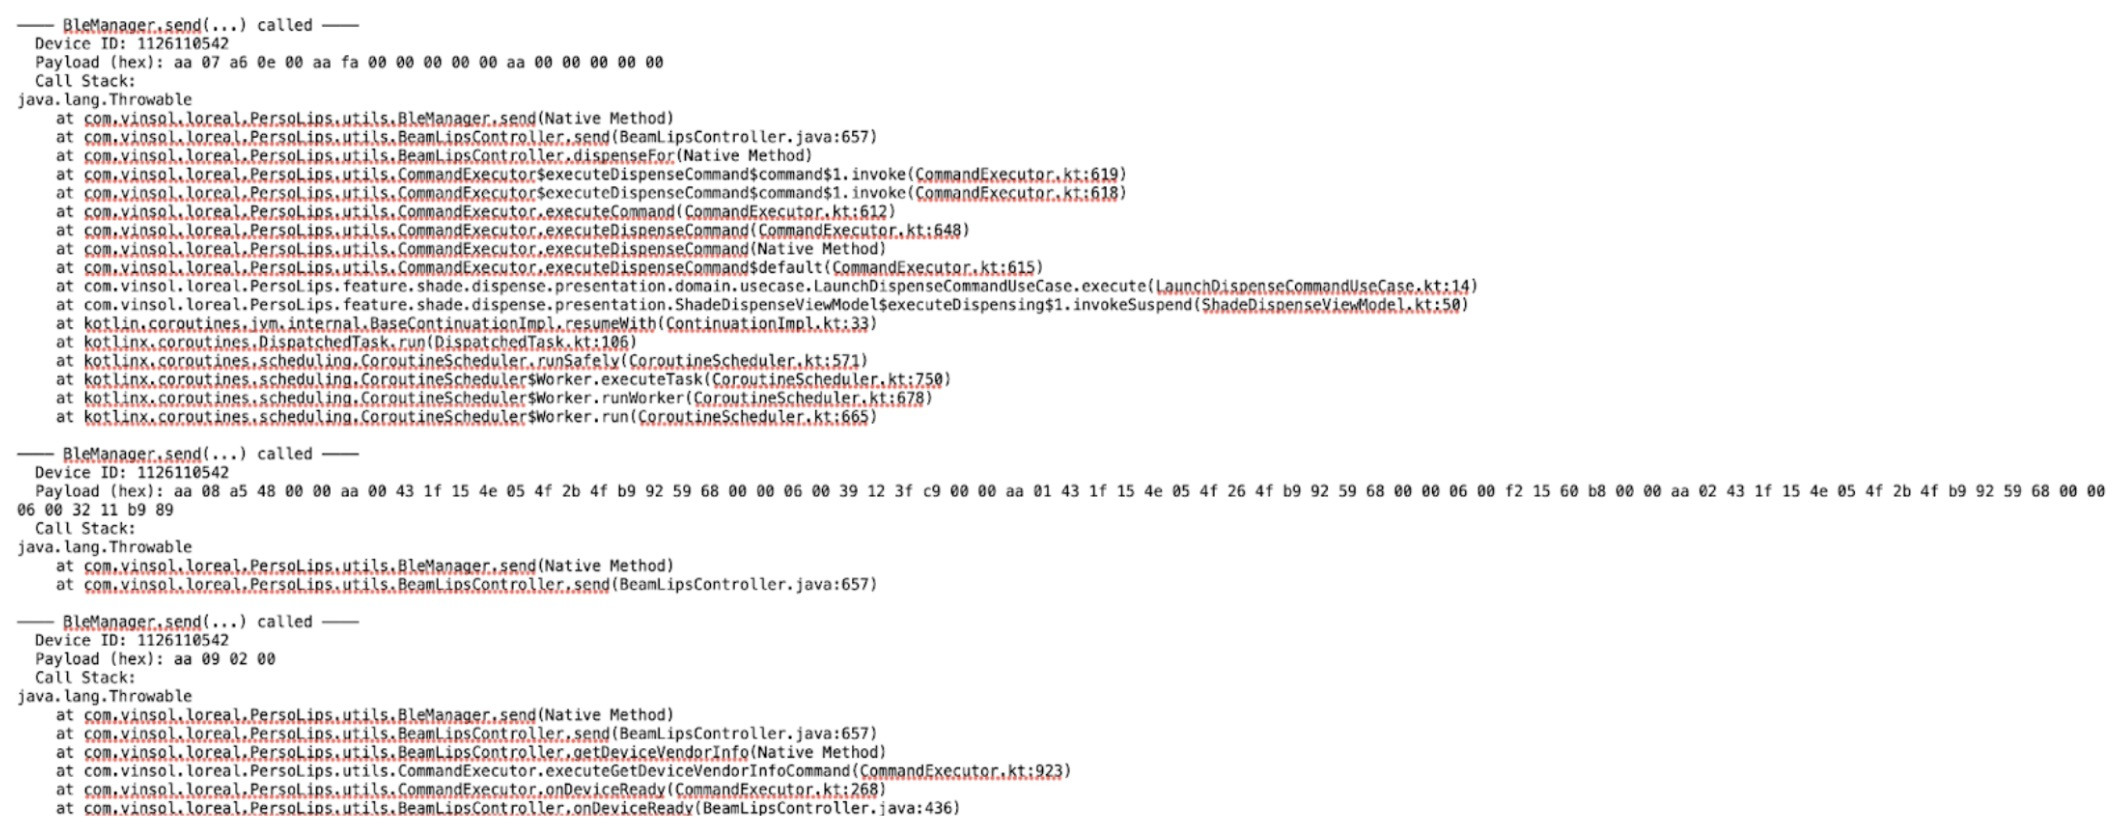
\includegraphics[width=0.7\linewidth]{hooked_payload}
	\caption{}
	\label{fig:hookedpayload}
\end{figure}

This stack trace offered strong clues about which packages to examine for more dispensing information. However, there was still a significant amount of investigation required. For example, the first method visible aside from send() was dispenseFor(). This is a native method, which means it is implemented in a language other than Java and compiled for a specific computer architecture, usually in C or C++. Native methods can access system-specific APIs not directly available in Java. According to IBM, “Native methods are Java™ methods that start in a language other than Java. Native methods can access system-specific functions and APIs that are not available directly in Java” (IBM, 2024). These methods are stored in .so files within the APK and cannot be decompiled with Dalvik bytecode decompilers like JADX. Instead, they must be reverse engineered from assembly-level code, which is possible but time-consuming. Because of this, I chose to focus on gathering more context through dynamic analysis rather than attempting to decompile the native code.  

To begin understanding the dispenseFor() function, I examined its declaration in JADX and logged its parameters. The only reference to it outside the executeDispense() function appeared in the BeamLipsController:

public native int dispenseFor(int i, String str, int i2, int i3, int i4, float f, int i5);

This signature provided insight into the types of variables used. The reference within executeDispense() offered a clearer picture of the parameters:

beamLipsController.dispenseFor(beamLipsDeviceId, colorUniverse, Color.red(color), Color.green(color), Color.blue(color), floatValue, intValue);

This helped identify the values that would need to be verified during testing. Below is the Frida hook I implemented to intercept calls to dispenseFor() and log the relevant information:

\begin{verbatim}
	// Hook dispenseFor(...)
	BeamLipsController.dispenseFor.overload(
	'int', 'java.lang.String', 'int', 'int', 'int', 'float', 'int'
	).implementation = function (deviceId, colorUniverse, r, g, b, vol, dose) {
		console.log("\n--- dispenseFor(...) called ---");
		console.log("  Device ID: " + deviceId.toString(16));
		console.log("  Color Universe: " + colorUniverse);
		console.log("  Red: " + r + " | Green: " + g + " | Blue: " + b);
		console.log("  Volume (float): " + vol + " → " + toHex(floatToBytes(vol)));
		console.log("  Dose (int): " + dose + " → " + toHex(intToBytes(dose)));
		console.log("  Call Stack (starting with exception):\n" +
		Log.getStackTraceString(Exception.$new()));
		logObjectFields(this);
		
		return this.dispenseFor(deviceId, colorUniverse, r, g, b, vol, dose);
	};
\end{verbatim}

And below is the resulting output from the test (excluding the call stack for brevity). 

\begin{verbatim}
	--- dispenseFor(...) called ---
	Device ID: 431f154e
	Color Universe: cool_nude
	Red: 228 | Green: 101 | Blue: 135
	Volume (float): 0.07999999821186066 -> 3d a3 d7 0a
	Dose (int): 1 -> 00 00 00 01
\end{verbatim}


\begin{tabular}{|l|l|l|l|}
	\hline
	\textbf{Field} & \textbf{Cartridge 0} & \textbf{Cartridge 1} & \textbf{Cartridge 2} \\ \hline
	Type & 00 & 00 & 00 \\ \hline
	PCrc16 & DBB13410 & 8E0746A3 & 258719E9 \\ \hline
	Volume & 4.165000 & 5.618000 & 4.084000 \\ \hline
	Crc16 & DD21 & CF18 & B1CC \\ \hline
	DeviceId & 431F154E & 431F154E & 431F154E \\ \hline
	TubeId & 0 & 1 & 2 \\ \hline
	Last use & 2025-06-26 01:29:16 & 2025-06-26 01:29:16 & 2025-06-26 01:29:16 \\ \hline
	Open date & 2025-05-20 08:00:00 & 2025-05-20 08:00:00 & 2025-05-20 08:00:00 \\ \hline
	End date & 2025-06-27 08:00:00 & 2025-06-22 08:00:00 & 2025-06-27 08:00:00 \\ \hline
	Exp. date & 2025-06-27 08:00:00 & 2025-06-22 08:00:00 & 2025-06-27 08:00:00 \\ \hline
	Formula id & MA\_513 & MA\_200 & MA\_100 \\ \hline
	Usable Vol. & 5.800000 & 5.800000 & 5.800000 \\ \hline
	Duration use & 730 & 730 & 730 \\ \hline
	Prod date & 2022-06-28 08:00:00 & 2022-06-23 08:00:00 & 2022-06-28 08:00:00 \\ \hline
	Batch id & 62W601 & 62W601 & 62W601 \\ \hline
	Color & 00DF75A0 & 006A2623 & 00C8725C \\ \hline
	Present? & 1 & 1 & 1 \\ \hline
	Up to date? & 1 & 1 & 1 \\ \hline
	Compatible? & 1 & 1 & 1 \\ \hline
	Opened? & 1 & 1 & 1 \\ \hline
	Expired? & 0 & 1 & 0 \\ \hline
	Empty? & 0 & 0 & 0 \\ \hline
	Valid? & 1 & 1 & 1 \\ \hline
	Virtual? & 0 & 0 & 0 \\ \hline
	CanDispense? & 1 & 1 & 1 \\ \hline
\end{tabular}

It is clear that much of the information required for the dispensing process is stored within the BeamLipsController object. While examining the JADX decompilation, I found that many of these fields also appear in the BeamLipsDevice model:

% TODO: \usepackage{graphicx} required
\begin{figure}[H]
	\centering
	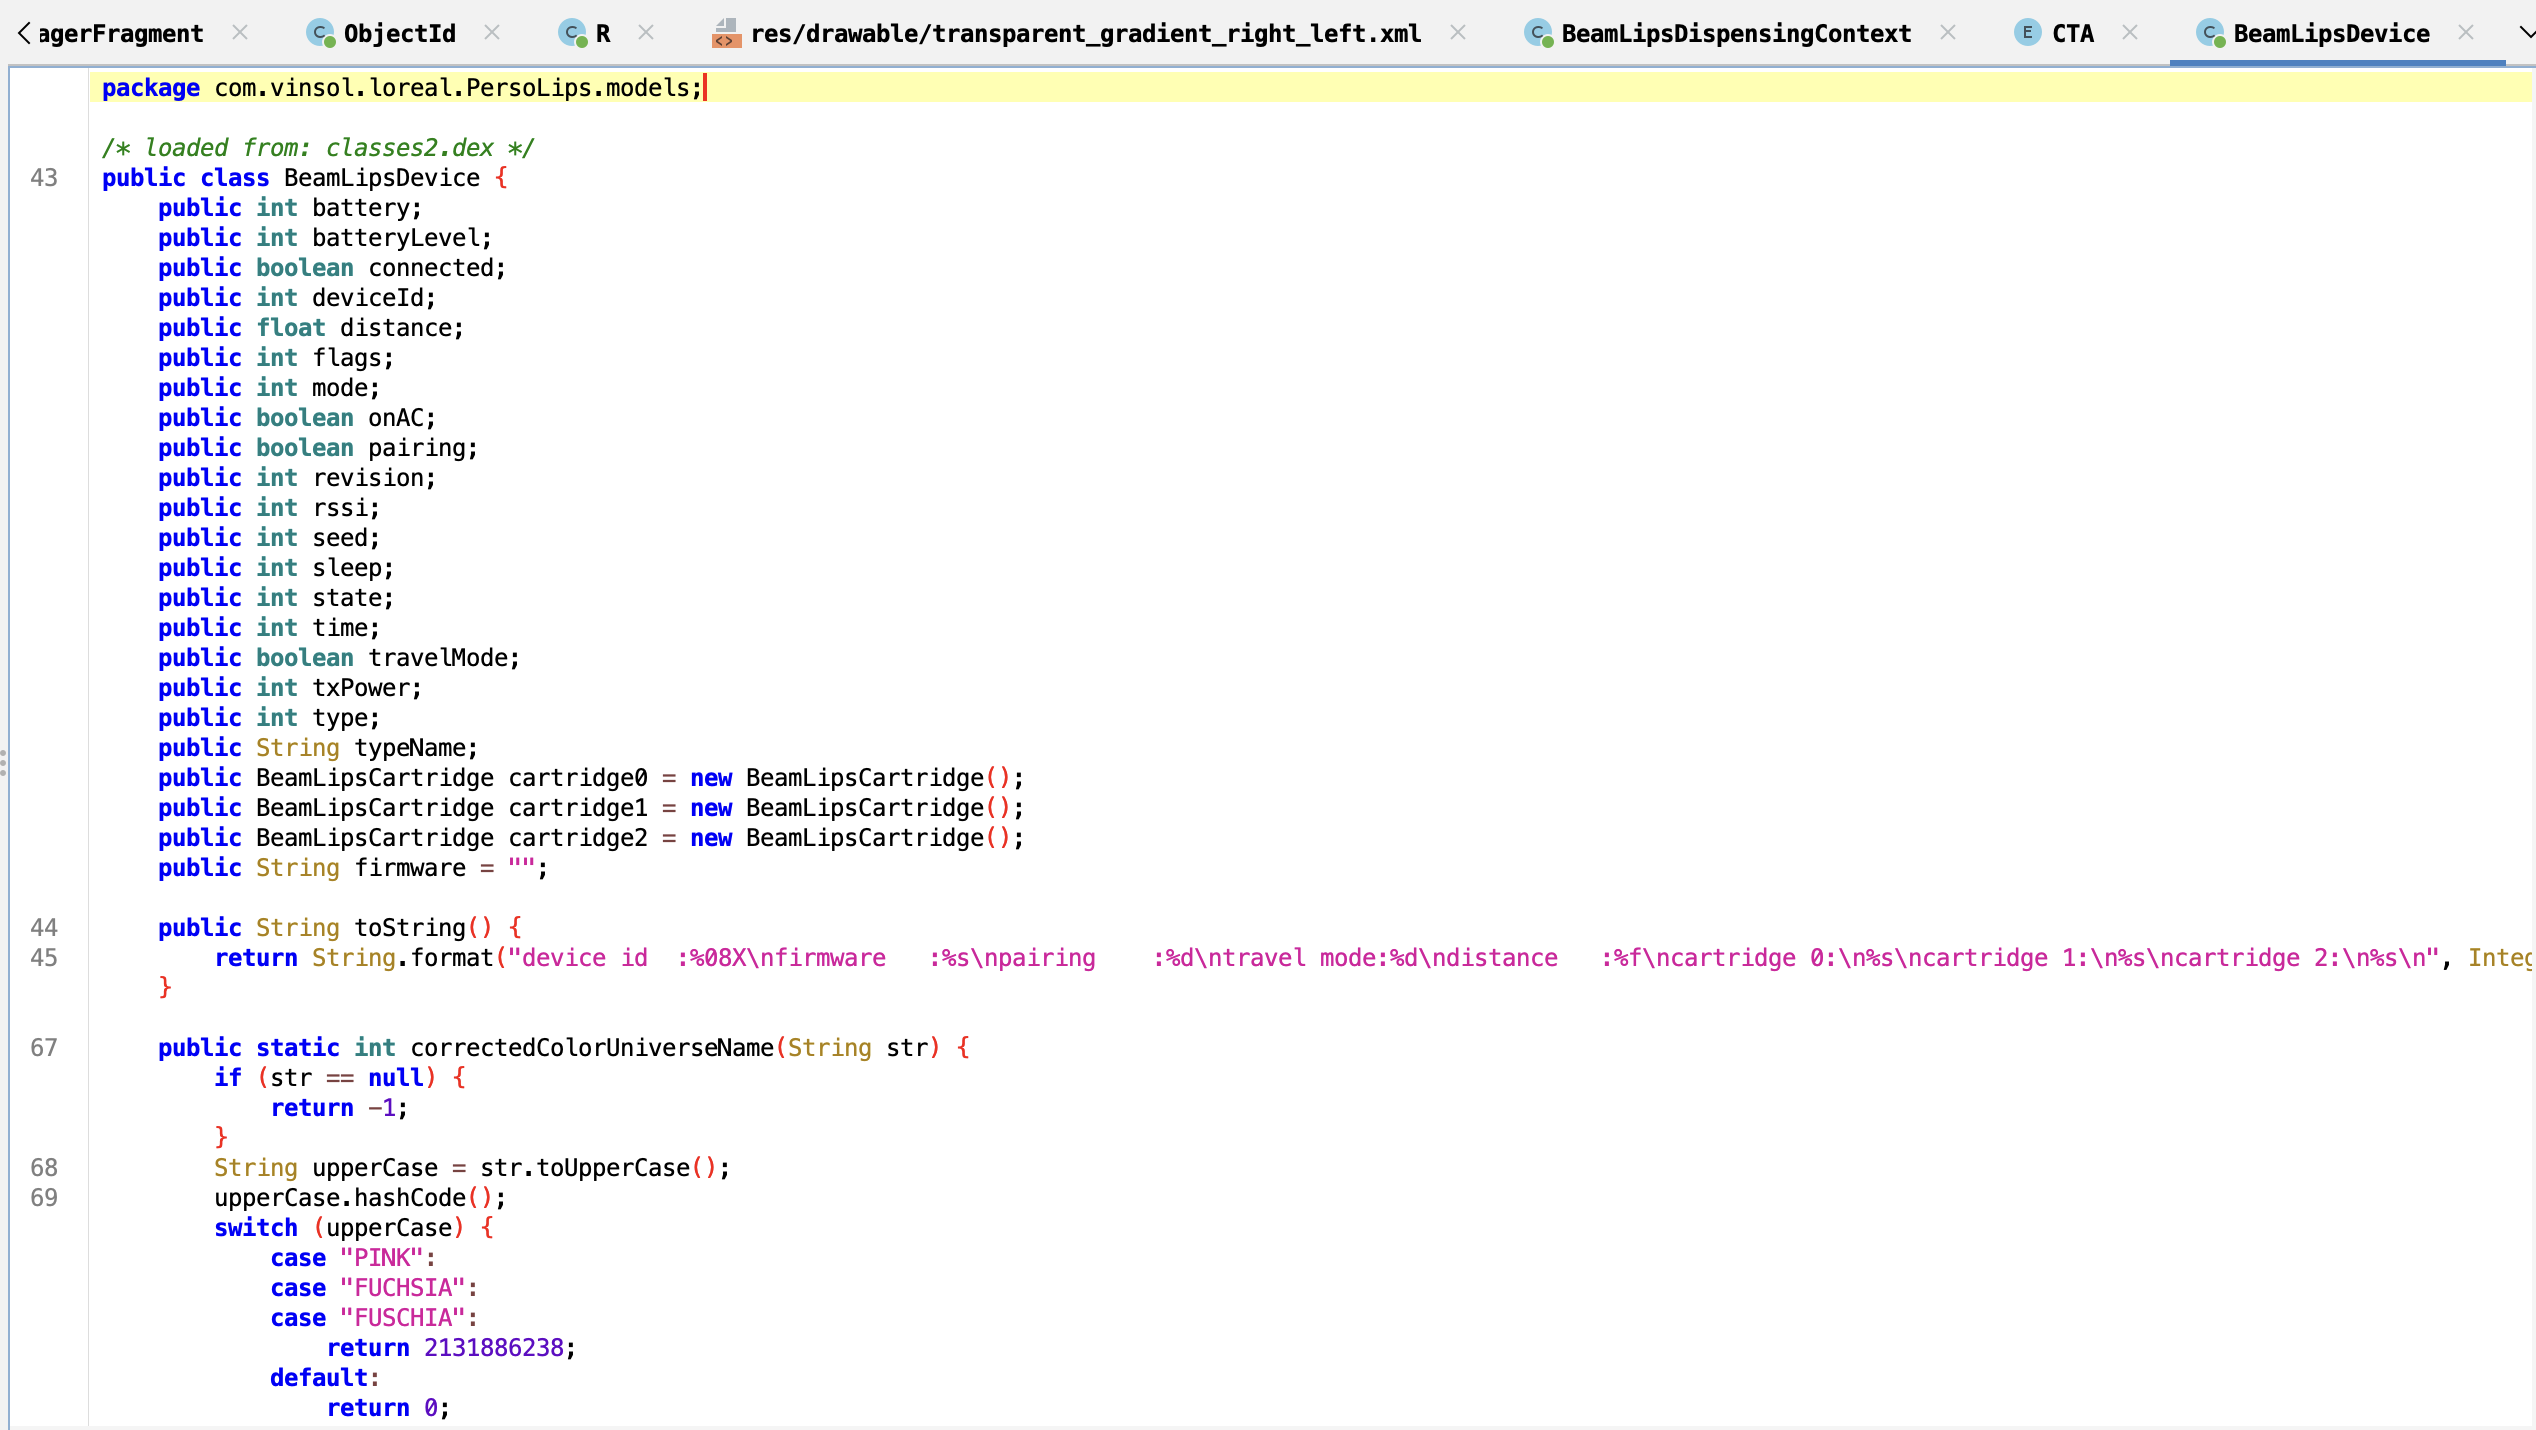
\includegraphics[width=0.7\linewidth]{beamlipsmodel}
	\caption{}
	\label{fig:beamlipsmodel}
\end{figure}

These variables provide valuable clues about what to look for in the raw payload. A crucial detail is that the device information appears to be divided into three cartridges, each maintaining its own set of data. Among the variables that seem particularly relevant to the dispense function are the usable volume, color, and dispense duration. I made note of these values to check whether they could be identified within the payload.

With these values hooked, the next step was to run tests and analyze the outcomes. After altering the variables, I was able to trace how specific values appeared in the payload. For example, the dispense payload associated with the dispenseFor hook revealed several important patterns:

% TODO: \usepackage{graphicx} required
\begin{figure}[H]
	\centering
	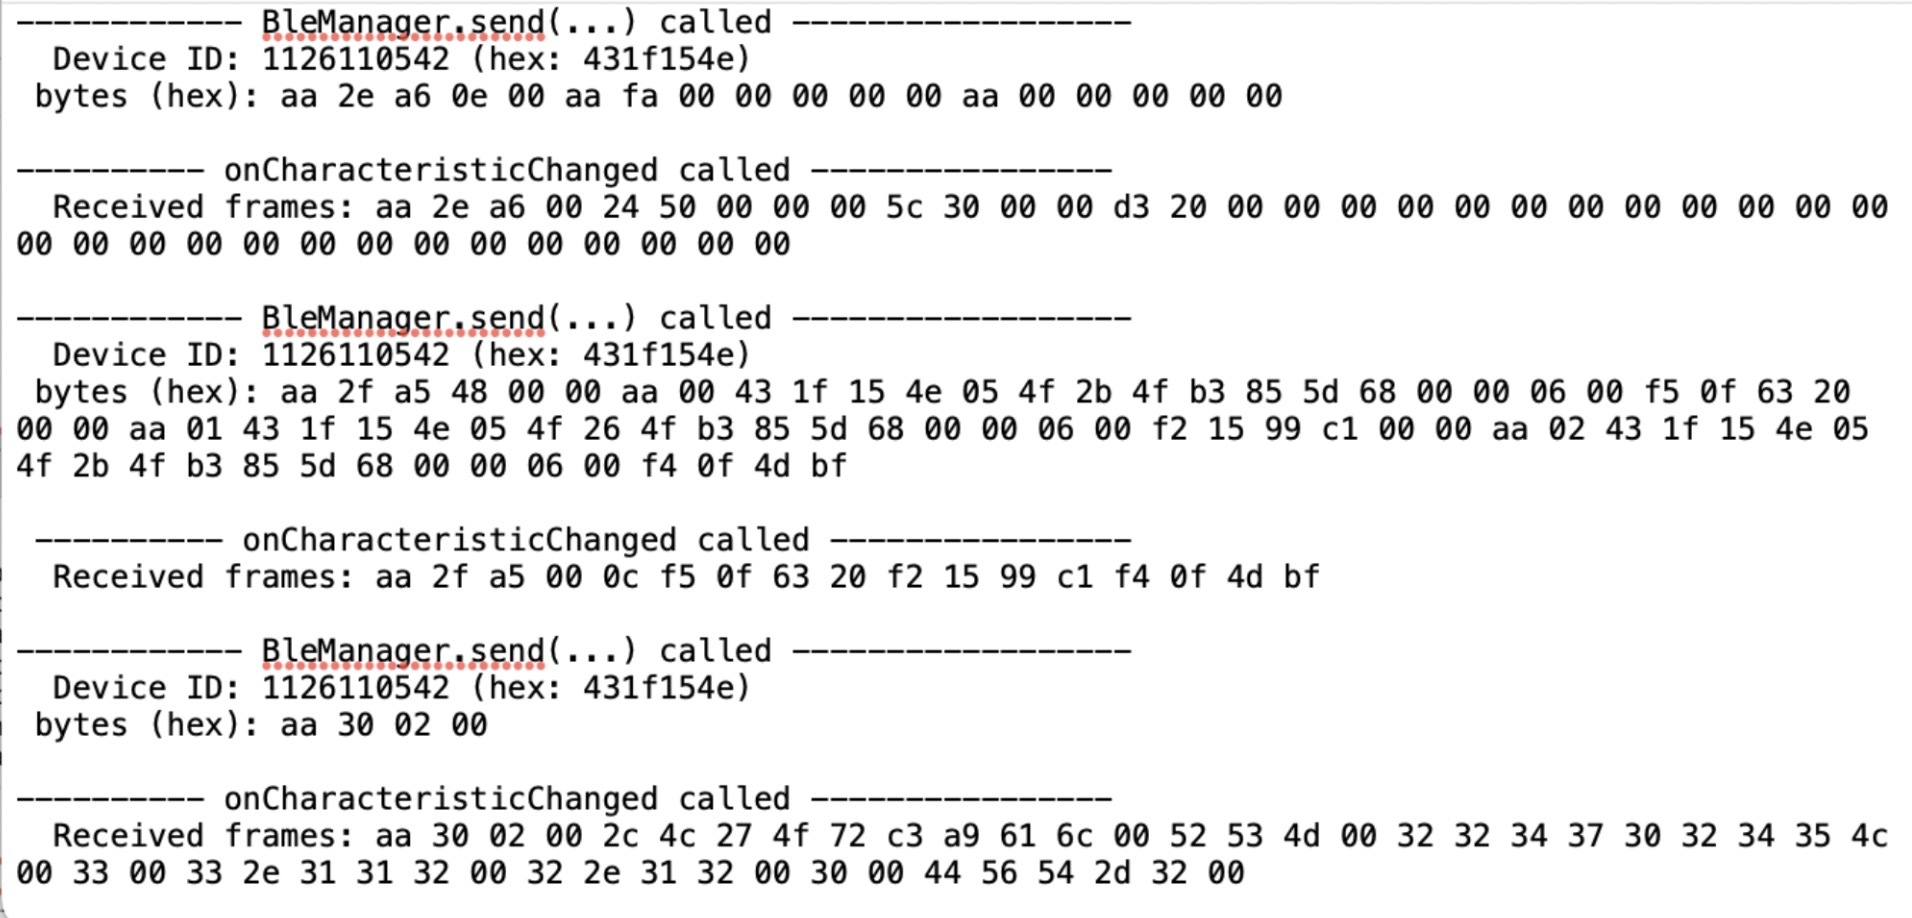
\includegraphics[width=0.7\linewidth]{payload1}
	\caption{}
	\label{fig:payload1}
\end{figure}

One of the first observations was that each send() transmission began with the byte aa, followed by a byte that incremented with each new message (e.g., 2e, 2f, 30). This indicates that the first two bytes of each payload likely serve as a counter to keep track of the sequence of transmitted packets. Additionally, after the app sends these two bytes (such as aa 2e), the device responds by writing back the same two bytes, further supporting the idea that this sequence acts as a counter and confirmation mechanism to ensure messages are being received in the correct order.

Another significant detail was that the device ID appeared three times in the second send() payload. Figure \ref{fig:deviceid} shows a screenshot of the device’s advanced settings screen from the app, which aligns with earlier findings from the hook indicating that the device splits its data into three channels, one for each cartridge. However, I continued investigating to determine whether any additional relevant information was present in the larger send() packet:

% TODO: \usepackage{graphicx} required
\begin{figure}[H]
	\centering
	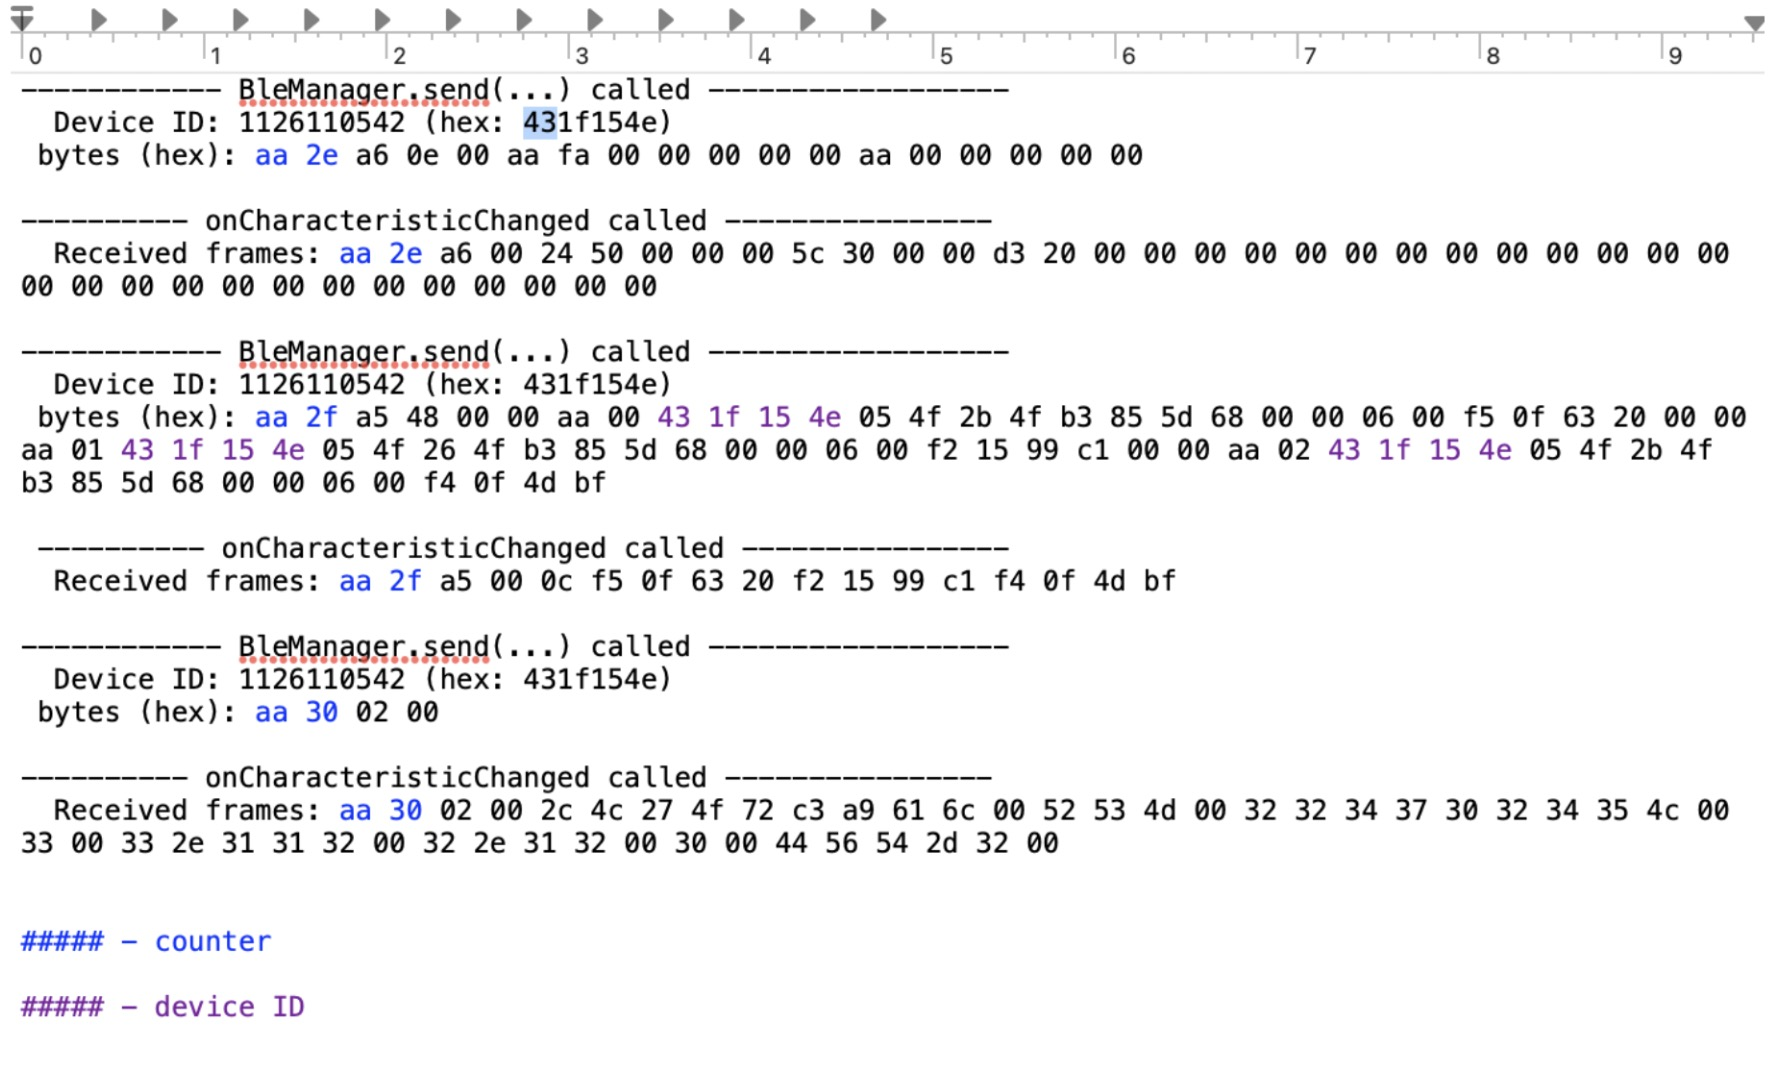
\includegraphics[width=0.7\linewidth]{payload2}
	\caption{}
	\label{fig:payload2}
\end{figure}

% TODO: \usepackage{graphicx} required
\begin{figure}[H]
	\centering
	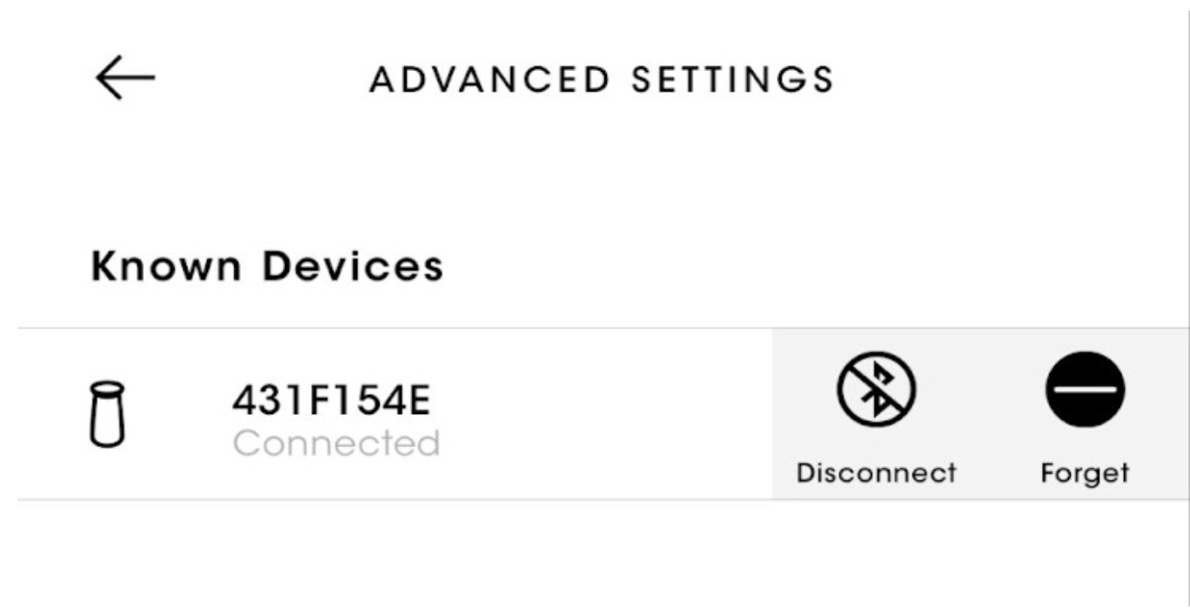
\includegraphics[width=0.7\linewidth]{device_id}
	\caption{}
	\label{fig:deviceid}
\end{figure}

Working from the hypothesis that the large send payload is organized by cartridge, I continued parsing through the data. As anticipated, I identified the patterns aa 00, aa 01, and aa 02 preceding each occurrence of the device ID, suggesting that the subsequent bytes are associated with data for each cartridge.

It is important to note that, while the information is presented here in a relatively straightforward manner, confirming each hypothesis required numerous tests and careful analysis:

% TODO: \usepackage{graphicx} required
\begin{figure}[H]
	\centering
	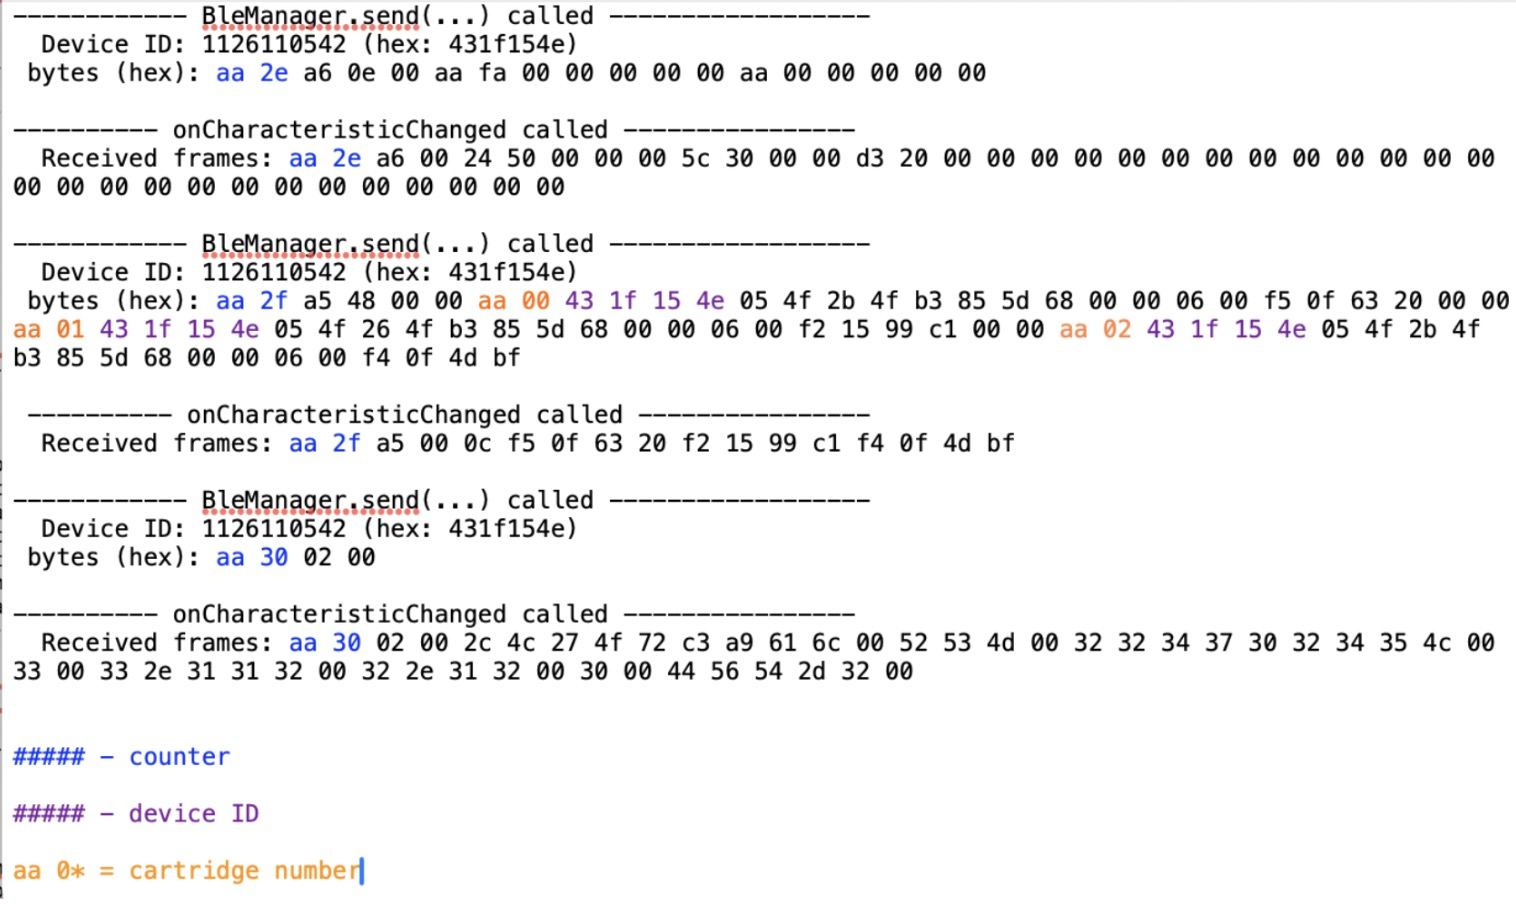
\includegraphics[width=0.7\linewidth]{payload3}
	\caption{}
	\label{fig:payload3}
\end{figure}

This is where the analysis began to grow more complex. To start, it’s important to understand the expected order in which the data appears. As a reminder, the send() and receive payloads under examination here are part of Bluetooth’s GATT profiles. According to the Bluetooth Core Specification 6, the GATT framework “defines procedures and formats of services and their characteristics. The procedures defined include discovering, reading, writing, notifying and indicating characteristics, as well as configuring the broadcast of characteristics” ~\cite{bluetooth2023}. The specification also states that “Multi-octet fields within the GATT profile shall be sent least significant octet first (little-endian) with the exception of the Characteristic Value field. The Characteristic Value and any fields within it shall be little-endian unless otherwise defined in the specification which defines the characteristic” ~\cite{bluetooth2023}. This indicates that much of the data should be expected in little-endian format.

Revisiting the payload, the next task was to determine where the dynamic data was stored. After running multiple tests, I identified a pattern in the dispense payloads: the four bytes immediately following 06 00 consistently changed, as did the four bytes preceding 00 00 06. This pattern suggests that these bytes contain data significant to the device and, therefore, crucial to decode if the goal is to replicate the dispense process with a custom payload. When decoding, these bytes can be grouped together, while fixed values can generally be treated as headers or spacers.

% TODO: \usepackage{graphicx} required
\begin{figure}[H]
	\centering
	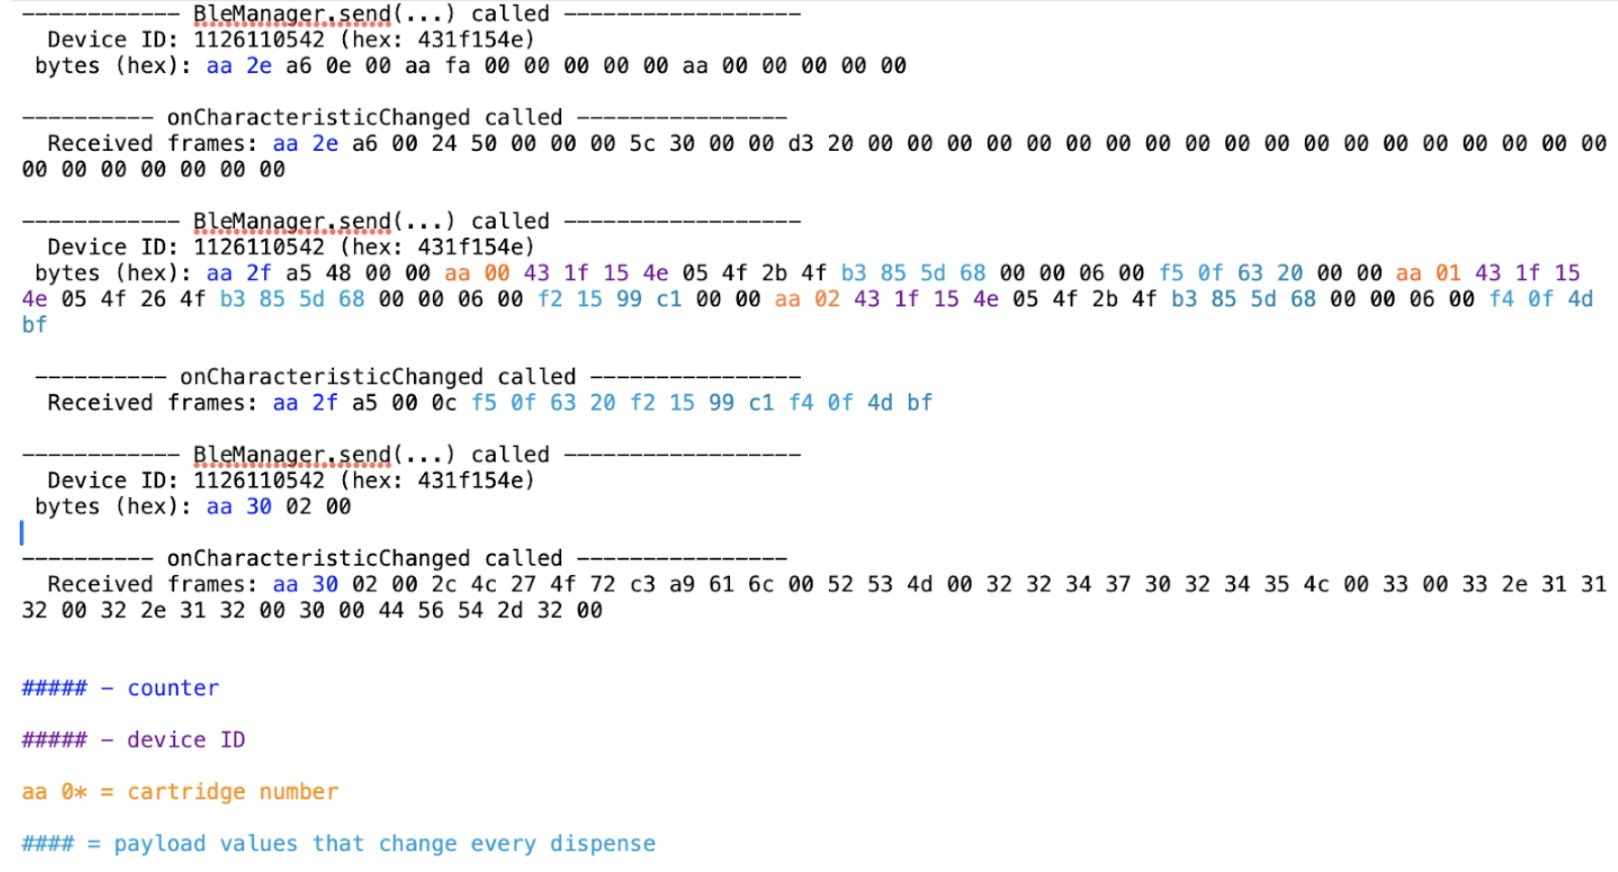
\includegraphics[width=0.7\linewidth]{payload4}
	\caption{}
	\label{fig:payload4}
\end{figure}

Using the cartridge data as a reference for what might appear in the larger payload, and knowing that volume is one of the most critical aspects of a dispense, I investigated whether the volume could be located within the payload. Because the volume changes between sends for the cartridges involved in dispensing, it was logical that the corresponding data would be part of the bytes that vary after each dispense. During testing, I noticed that when dispensing from only one cartridge, just two bytes would change within one of the four-byte sequences, while the remaining bytes stayed constant across dispenses. With a strong hypothesis about which bytes were significant, the next step was to test various ways these bytes could represent the volume information.

Identifying the correct data took several attempts. One significant obstacle was that, initially, I focused on locating the dispense volume itself, rather than recognizing that the volume 
appeared as the current total volume within each cartridge. Once I connected that I should be looking for information in the cartridge data, representing the total volume per cartridge, and recalled that Android systems generally encode data in little-endian, the discovery became much clearer. Figure \ref*{fig:payload5} illustrates the calculation of the volume derived from the payload.

% TODO: \usepackage{graphicx} required
\begin{figure}[H]
	\centering
	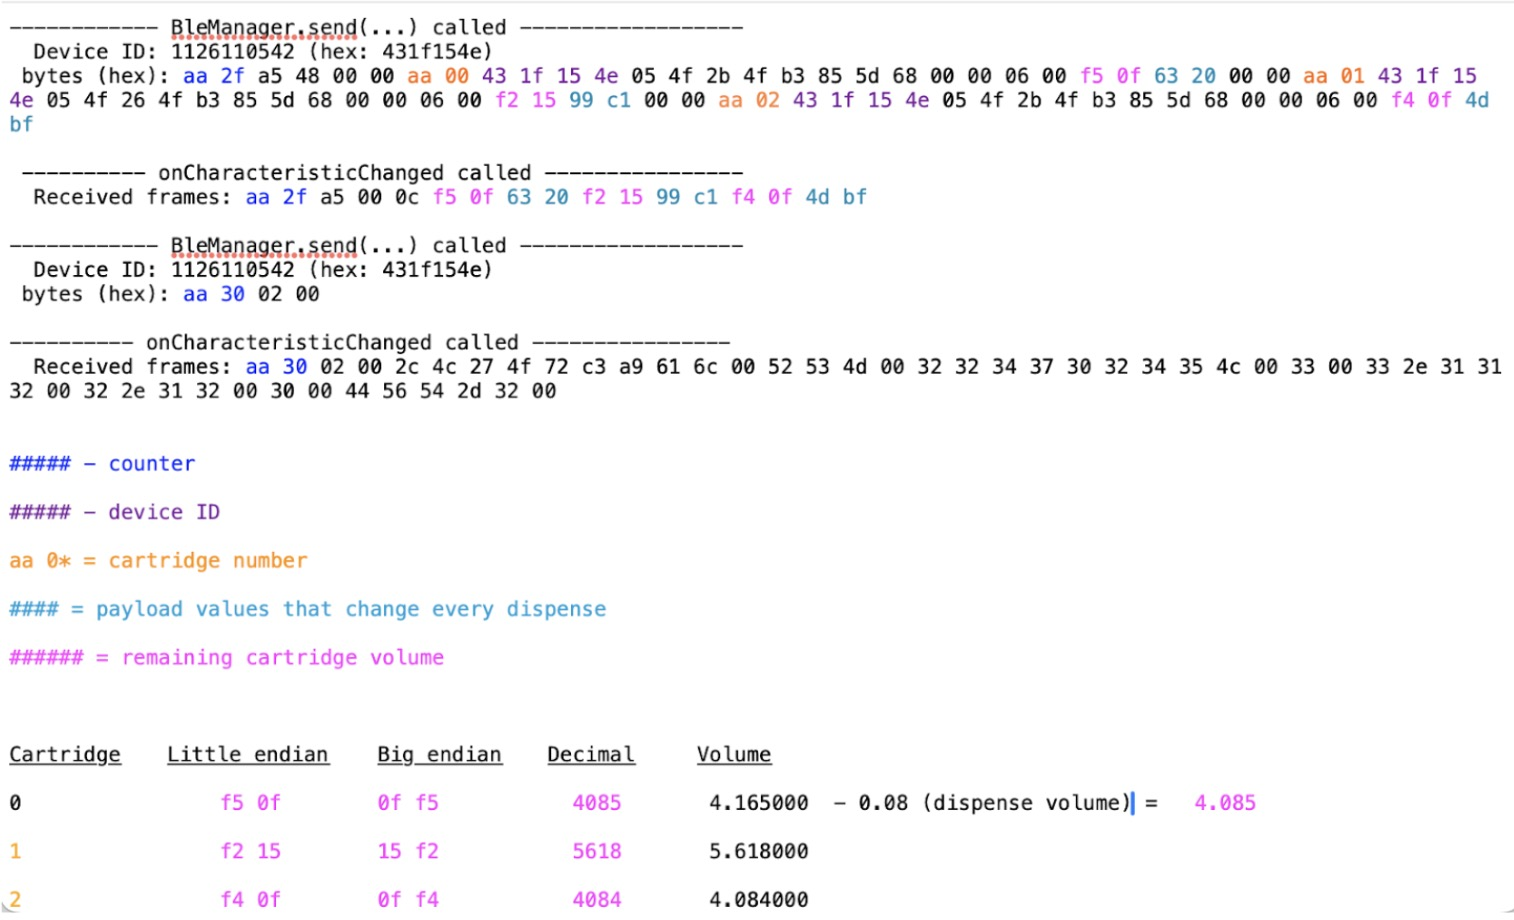
\includegraphics[width=0.7\linewidth]{payload5}
	\caption{}
	\label{fig:payload5}
\end{figure}

After decoding the volume, there remained only one four-byte sequence and one two-byte sequence whose purposes were still unknown. To identify these, I revisited the cartridge information for additional clues. One recurring element in the cartridge data was information related to dates. Based on that insight, I experimented with reversing various combinations of bytes into big-endian format and using Python to convert these values into UTC datetime stamps. Ultimately, the full four-byte sequence before 00 00 06 was found to translate to the current print time.

% TODO: \usepackage{graphicx} required
\begin{figure}[H]
	\centering
	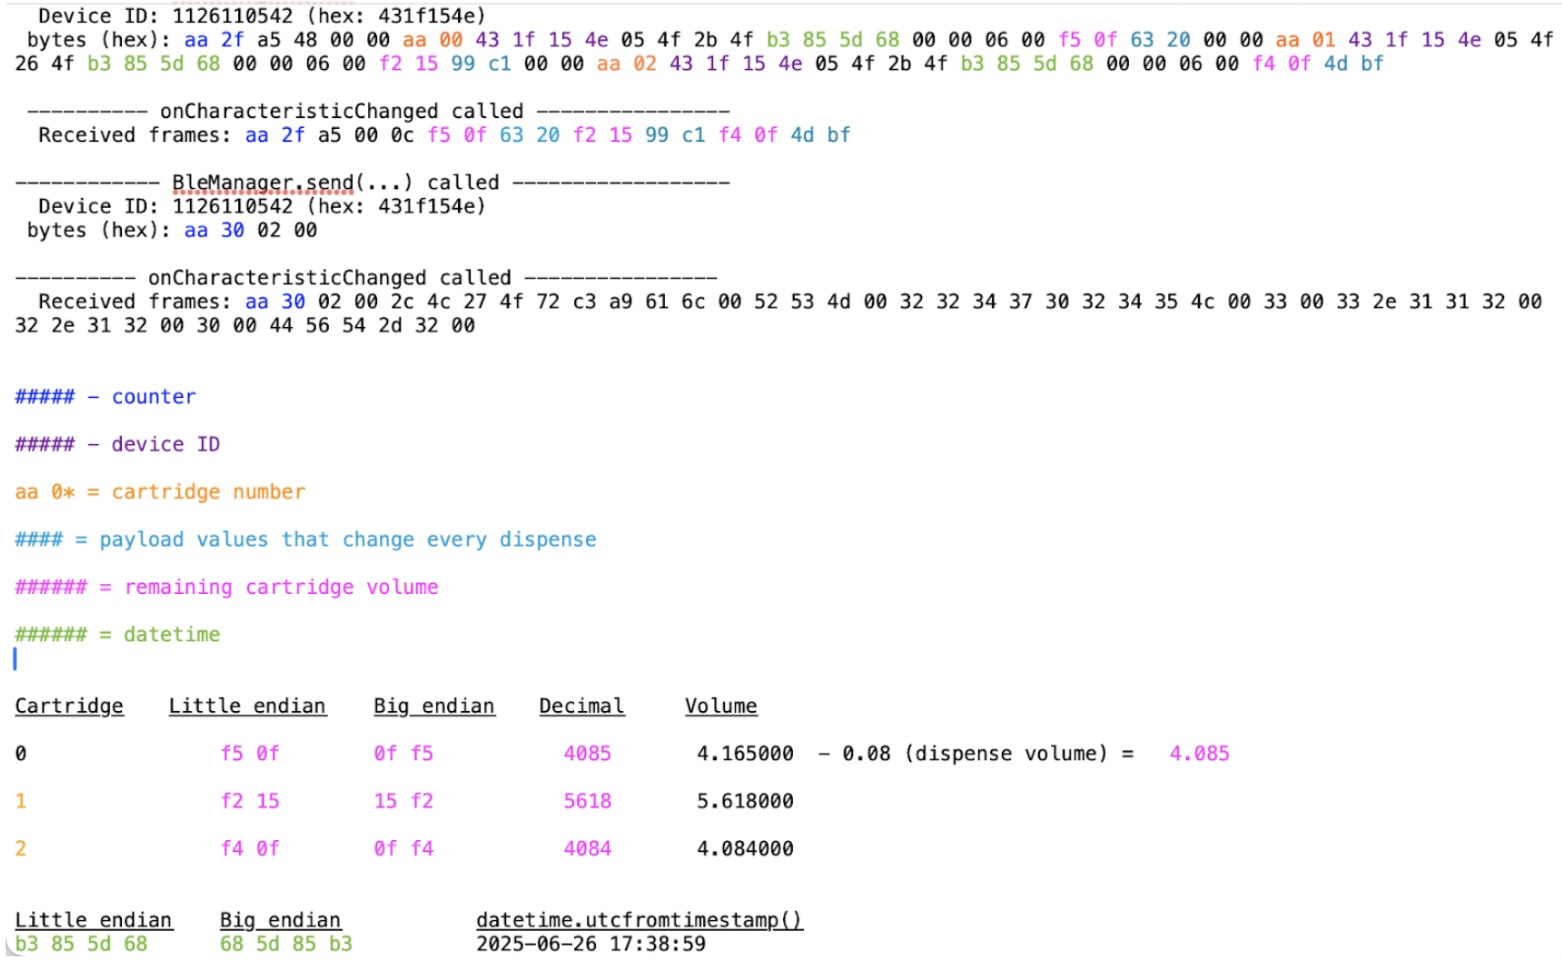
\includegraphics[width=0.7\linewidth]{payload6}
	\caption{}
	\label{fig:payload6}
\end{figure}

This is the extent of what I was able to decode during the timeframe of this project. The amount of information discovered would likely be sufficient for me to attempt spoofing the byte data to the device, using random values for the final two-byte sequences that remain undecoded (the bytes shown in teal). However, given the time constraints of the project, I chose instead to attempt a simpler approach first. My plan was to leverage the information gathered from hooking the functions to carry out a man-in-the-middle strategy.

Despite this shift in strategy, all the insights from analyzing the payloads remain valuable, as they help clarify the types of information the device expects to receive. This data has been documented for possible future use in crafting spoofed payloads. Figure \ref{fig:bigpayload} shows one of my comprehensive tests analyzing the byte payload from a pink dispense.

% TODO: \usepackage{graphicx} required
\begin{figure}[H]
	\centering
	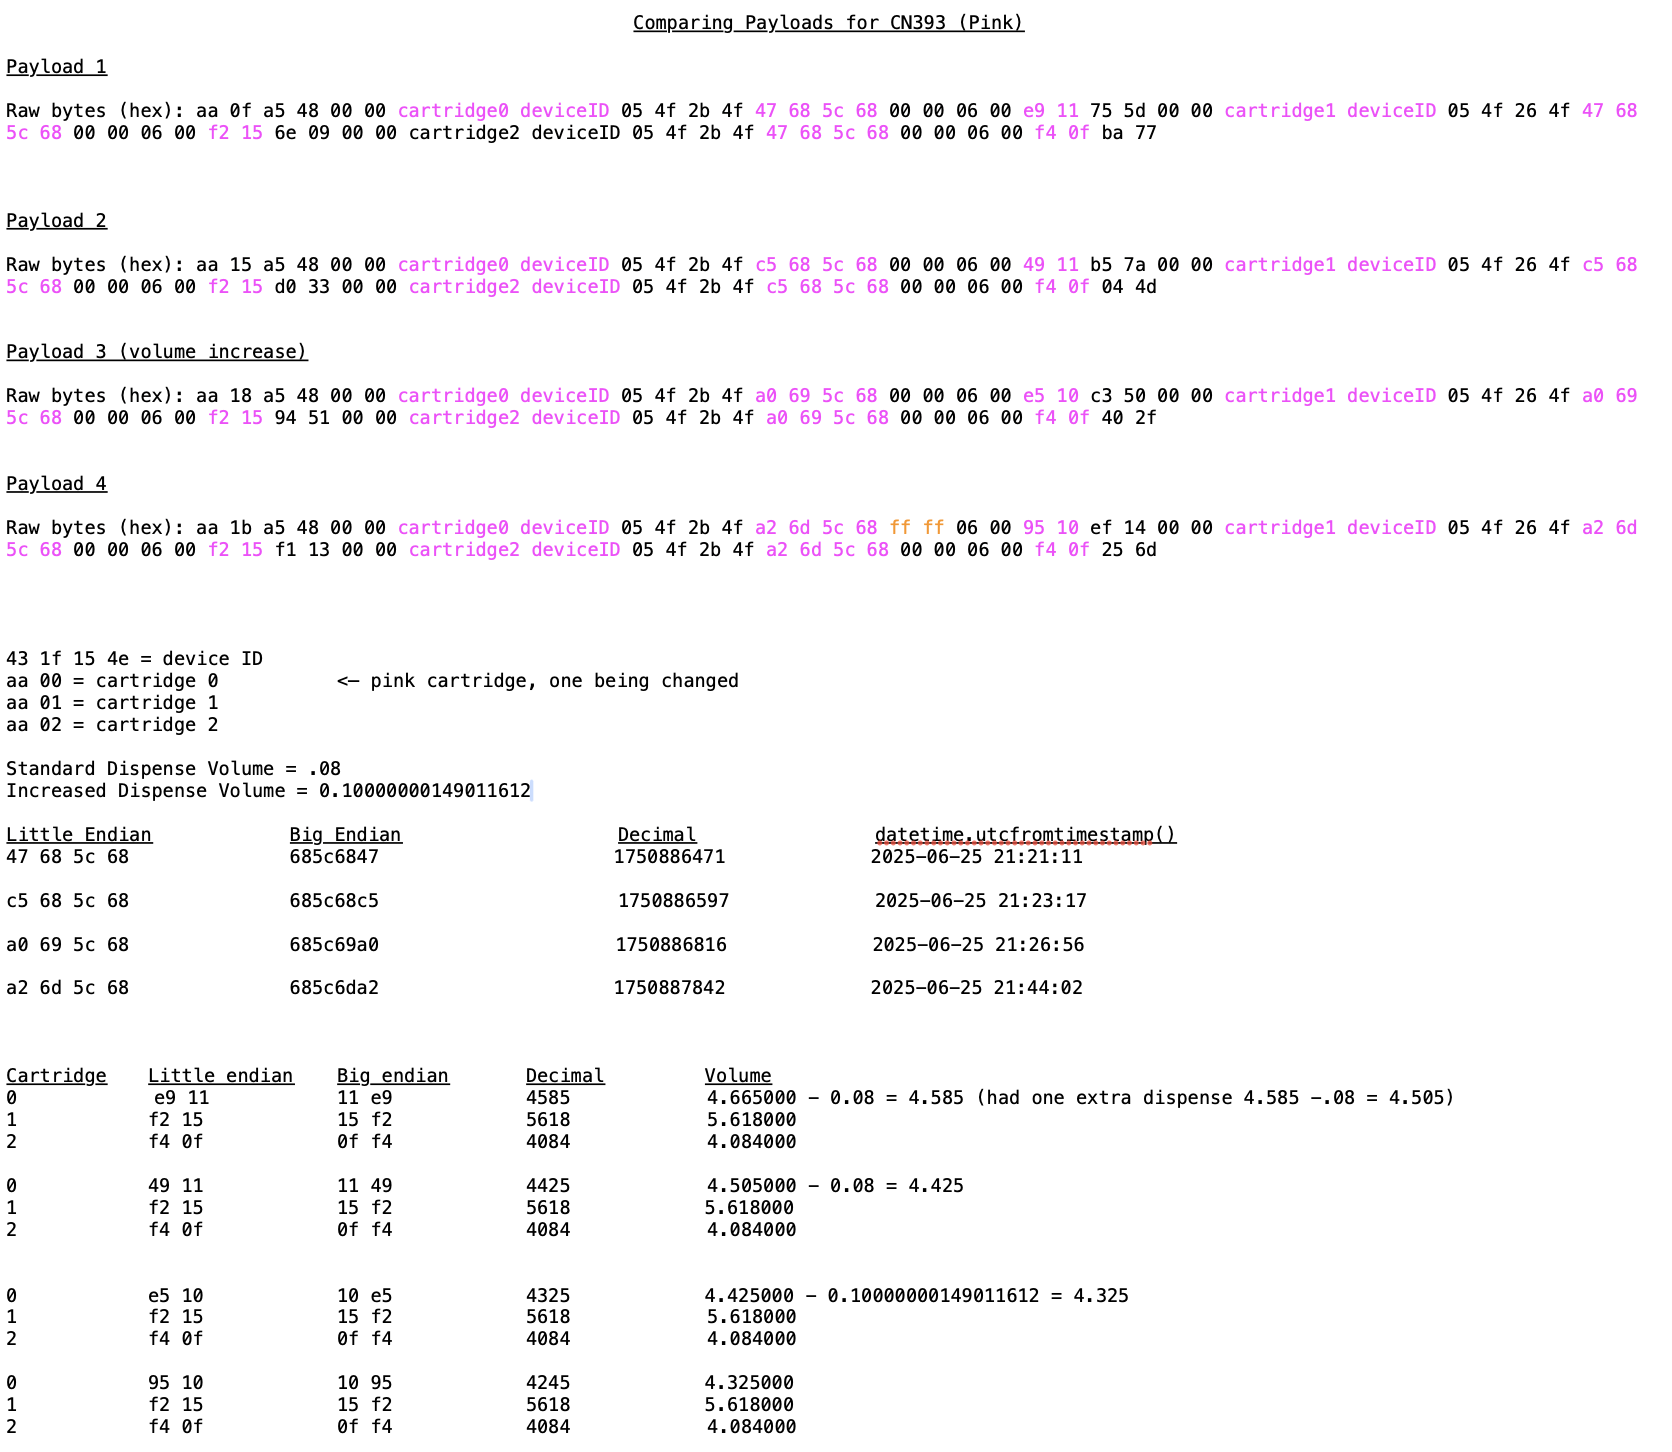
\includegraphics[scale=.3]{bigpayload}
	\caption{}
	\label{fig:bigpayload}
\end{figure}


\section{Executing the Dispense}
With the comprehensive data gathered from earlier experiments, I set out to modify the color parameters and initiate a dispense. I once again used Frida’s straightforward Java method hooks, but in this iteration I directly manipulated the input variables of the dispenseFor() function. For clarity, the method signature is:

beamLipsController.dispenseFor(beamLipsDeviceId, colorUniverse, Color.red(color), Color.green(color), Color.blue(color), floatValue, intValue);

This function receives the cartridge universe identifier, the red, green, and blue components of the selected shade, the volume to dispense, and the dose count. My objective is to demonstrate the capacity to override these values at runtime. To achieve this, I redirected a dispense request originally set to light pink so that it produced a light brown output instead. Figure \ref{fig:environmentsetup} depicts the test arrangement, highlighting device connections and the sequence of operations.

% TODO: \usepackage{graphicx} required
\begin{figure}[H]
	\centering
	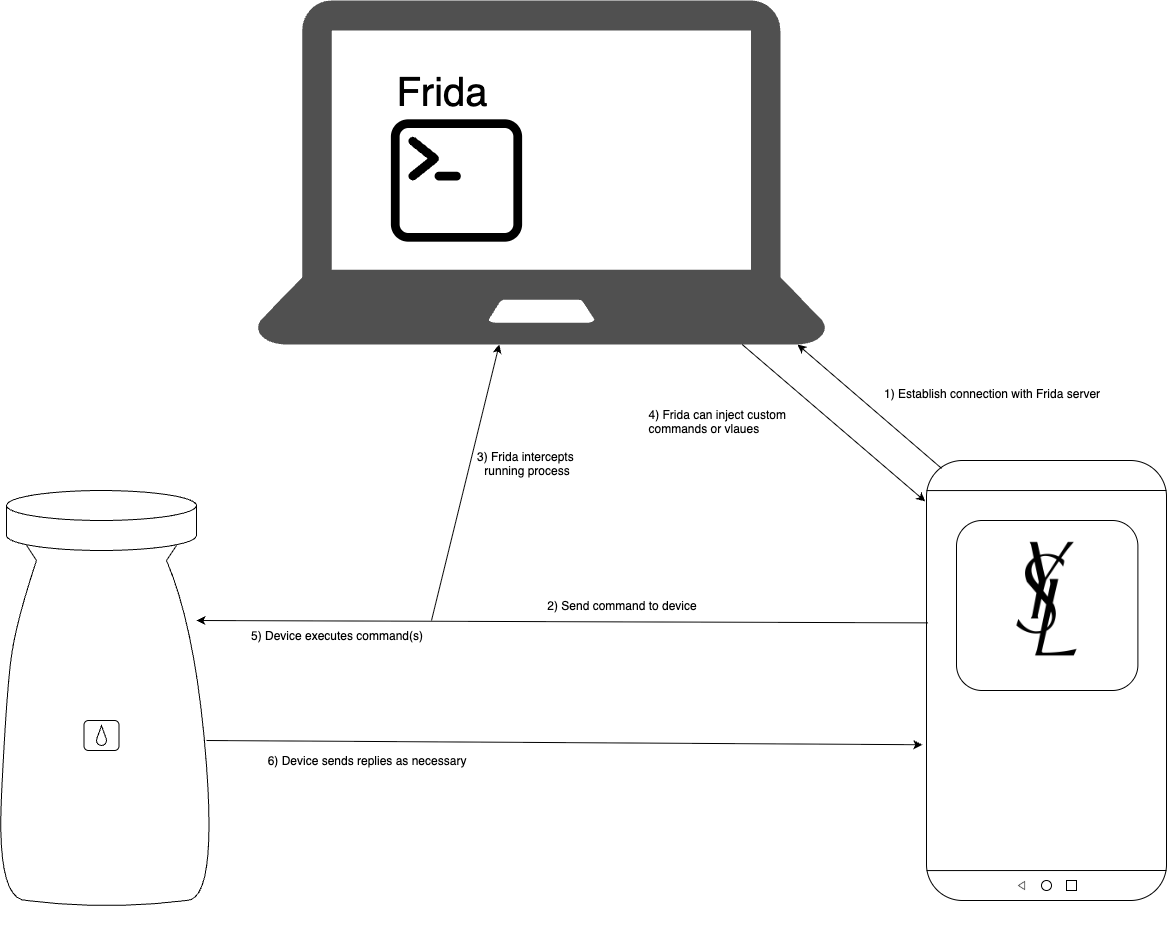
\includegraphics[width=0.7\linewidth]{environmentsetup}
	\caption{}
	\label{fig:environmentsetup}
\end{figure}

The Frida script follows the same pattern as previous hooks. First, I capture and log each incoming parameter to verify the original settings. I then replace the RGB values with those corresponding to the CN24 light brown shade, which are 200, 114, and 92 based on an earlier hook session. Finally, I invoke the original method with the modified values. The full script is presented below:

\begin{verbatim}
	Java.perform(function () {
		var BeamLipsController = Java.use("com.vinsol.loreal.PersoLips.utils.BeamLipsController");
		var overload = BeamLipsController.dispenseFor.overload(
		'int',
		'java.lang.String',
		'int',
		'int',
		'int',
		'float',
		'int'
		);
		
		overload.implementation = function(deviceId, colorUniverse, red, green, blue, volume, dose) {
			console.log("\n=== dispenseFor(...) called ===");
			console.log("Device ID: " + deviceId);
			console.log("Color Universe: " + colorUniverse);
			console.log("Original Red: " + red);
			console.log("Original green: " + green);
			console.log("Original Blue: " + blue);
			console.log("Original volume: " + volume);
			console.log("Original dose: " + dose);
			
			console.log("---------------------- Altering Color Values to print CN24 -------------------------");
			
			red = 200;
			green = 114;
			blue = 92;
			
			console.log("Modified Red: " + red);
			console.log("Modified Green: " + green);
			console.log("Modified Blue: " + blue);
			
			return overload.call(
			this,
			deviceId,
			colorUniverse,
			red,
			green,
			blue,
			volume,
			dose
			);
		};
		
		console.log("*** Hooked correct overload of dispenseFor in BeamLipsController ***");
	});
\end{verbatim}

The result was incredibly exciting. As shown in Figure \ref{fig:dispenseprint}, the device produced a light brown swatch even though the app remained set to light pink. However, the original light pink also appeared alongside the brown, despite only a single invocation of the modified dispenseFor() call. Furthermore, the final shade reported was CN63—a brown-pink hybrid that does not exist on the official color wheel (see Figure \ref{fig:cn63}).
% TODO: \usepackage{graphicx} required
\begin{figure}[H]
	\centering
	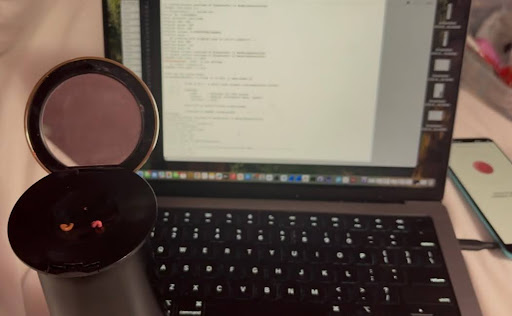
\includegraphics[scale=.7]{dispenseprint}
	\caption{}
	\label{fig:dispenseprint}
\end{figure}
% TODO: \usepackage{graphicx} required
\begin{figure}[H]
	\centering
	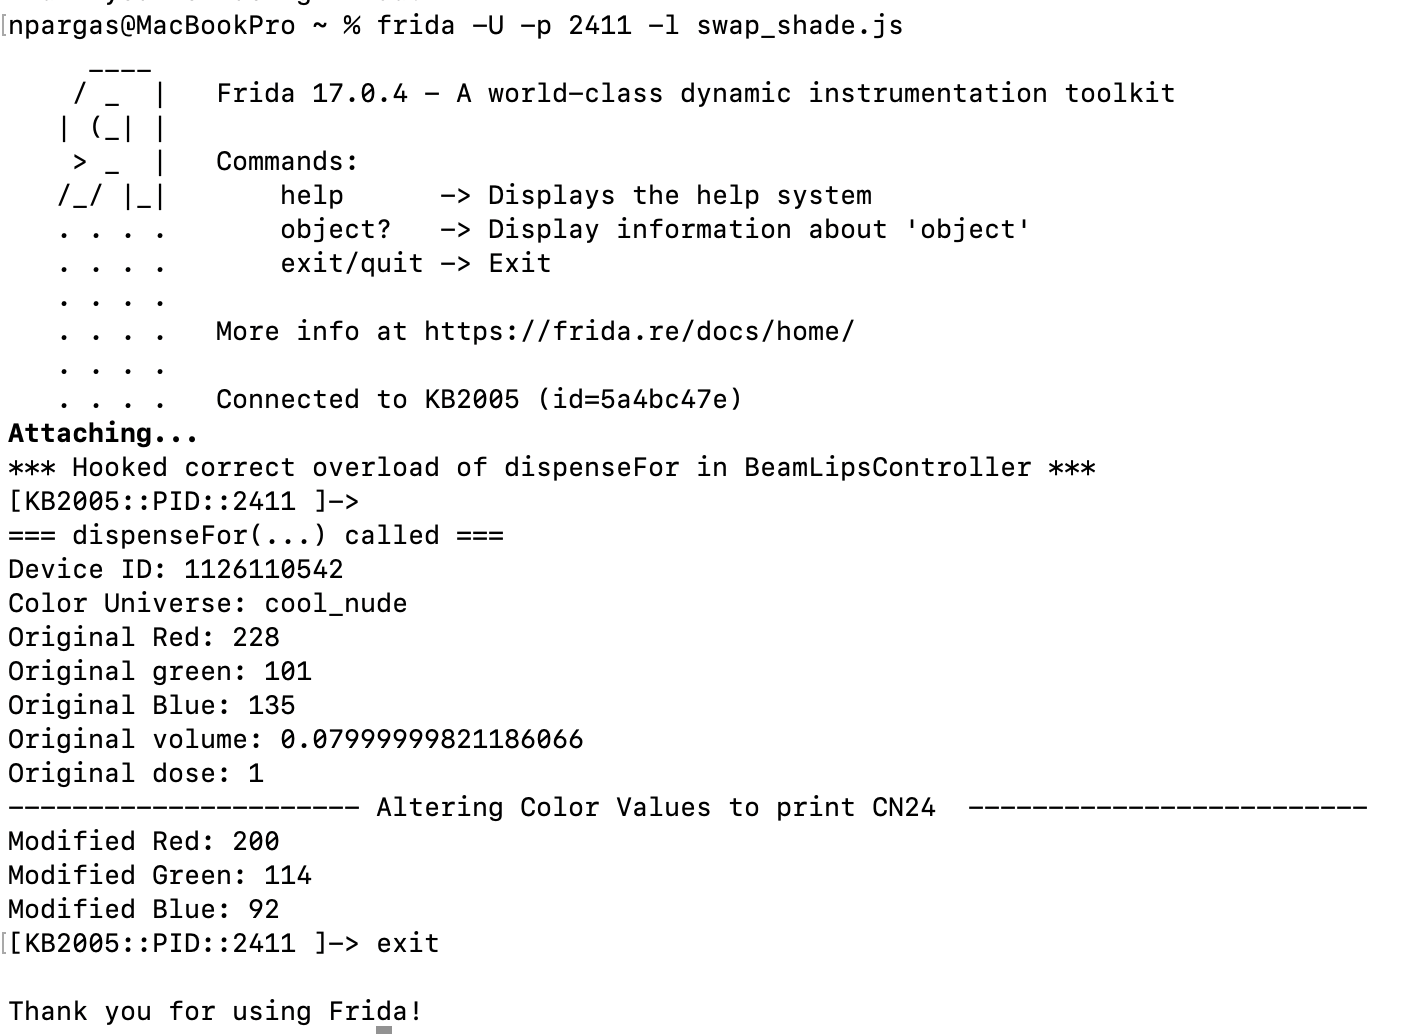
\includegraphics[scale=.15]{swapshadefrida}
	\caption{}
	\label{fig:swapshadefrida}
\end{figure}

% TODO: \usepackage{graphicx} required
\begin{figure}[H]
	\centering
	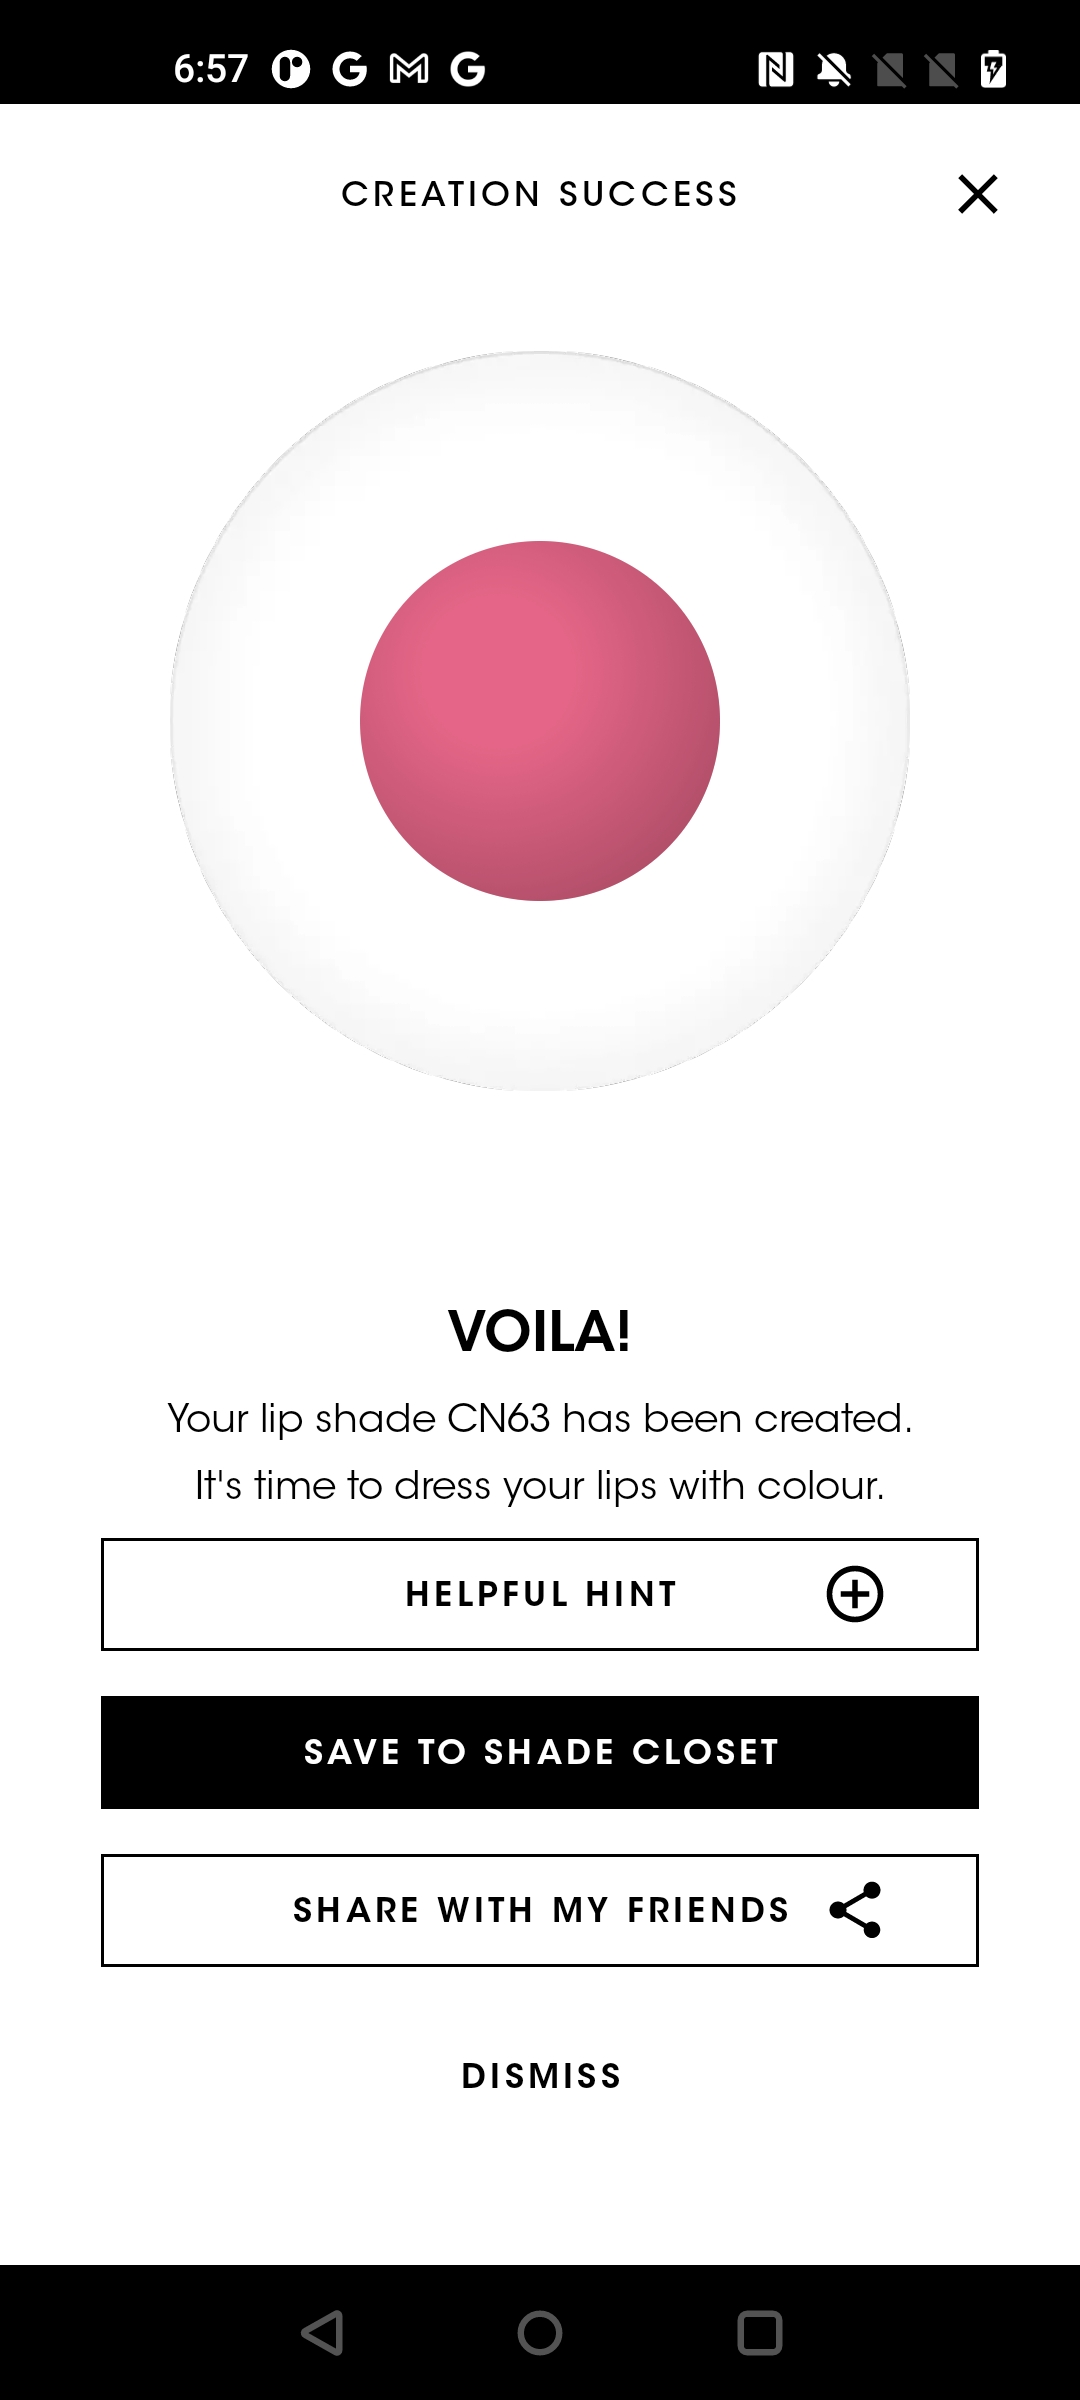
\includegraphics[scale=.15]{cn63}
	\caption{}
	\label{fig:cn63}
\end{figure}

These findings indicate that additional processing occurs after the RGB parameters are accepted. Possible explanations include internal blending algorithms, use of cached color values, or fallback logic within the application or firmware. To uncover the precise source of these effects, I could trace subsequent method calls and capture post-dispense data packets in future experiments


%%!TEX root = ../main.tex
\chapter{Conclusion}
\section{Conclusion}
This project has undertaken a comprehensive investigation of reverse engineering practices as applied to complex Bluetooth‑enabled systems. By examining both theoretical foundations and practical implementations, we have illuminated the interplay between static code analysis, dynamic instrumentation, and wireless packet inspection. Our objective was twofold: to understand the internal architecture of a commercial Android application that communicates with a Bluetooth peripheral and to demonstrate the feasibility of intercepting and manipulating its behavior in real time.
First, static analysis using JADX provided a crucial starting point for mapping the application’s data flow and identifying key functions. Through systematic decompilation and code review, we traced how user inputs and device commands are translated into Bluetooth payloads. This phase revealed the structure of the proprietary protocol and established a blueprint for subsequent dynamic testing. However, static techniques alone cannot capture runtime behaviors such as input validation, encryption routines, or environment‑specific logic.
To address these limitations, we employed Frida for dynamic instrumentation. By injecting hooks into the application’s Java methods, we were able to observe live function calls, inspect variable values, and modify parameters before transmission. Frida’s versatility enabled close inspection of runtime behavior and the execution of targeted manipulations, confirming that the application’s control logic could be influenced without source‑level modifications. This dynamic approach complemented the insights gained from static decompilation and provided definitive evidence of our capacity to alter an application’s operation.
Complementing code‑centric methods, Bluetooth packet sniffing yielded an unambiguous record of over‑the‑air exchanges between the mobile application and the peripheral device. Using a hardware sniffer and analysis software, we captured raw packets that corroborated the structure inferred from code review and Frida instrumentation. These traces ensured that our reverse‑engineering conclusions were grounded in empirical measurements rather than extrapolation. The integration of packet‑level data with code‑level insights formed a robust, end‑to‑end understanding of the entire communication pipeline.
Throughout this work, an iterative methodology proved essential. Each new discovery prompted reevaluation of prior assumptions and guided subsequent experiments. Establishing a reliable environment—including rooted devices and virtual machines—facilitated rapid prototyping and reproducibility. Equally important was meticulous documentation of all procedures, findings, and hypotheses, which preserved critical knowledge and supported collaborative scrutiny.
In sum, this project demonstrates that commercial‑grade Bluetooth applications can be effectively reverse engineered through a judicious combination of static analysis, dynamic instrumentation, and packet monitoring. The techniques and workflows developed here provide a foundation for further research into more advanced protocols and emerging hardware platforms. By refining automation tools and expanding coverage to additional communication layers, future work can continue to push the boundaries of applied reverse engineering within the security research community.

\section{Future Work}
The current study has demonstrated that manipulating the dispense process of the device is not only possible but can serve as a robust foundation for achieving comprehensive command over its functions. Building upon these initial findings, the next phase of research could refine communication protocols, reverse‑engineer proprietary algorithms, develop a standalone application, and analyze firmware to uncover hidden operational logic.
First, building on the initial packet capture efforts conducted during this study, the research could return to in‑depth Bluetooth packet analysis to further elucidate the device’s communication protocol. This effort might involve capturing and parsing additional raw GATT traffic to confirm previously observed services, characteristics, and command sequences. Using tools such as Wireshark or specialized BLE sniffers, the study could refine documentation of packet structures, attribute handles, and payload formats. 
Second, additional efforts could concentrate on isolating and interpreting the device’s color-related commands within the captured Bluetooth packets. This would involve identifying specific GATT characteristics or payload patterns that correspond to shade adjustments, enabling direct control over pigment ratios without requiring extensive algorithmic reconstruction.
Third, with both communication protocols and color models established, the research could focus on developing a standalone mobile application independent of the vendor’s software. This application could include detailed documentation of the Bluetooth services and characteristics, such as UUIDs, properties, and data formats, required to interface with the device. The user interface could then offer intuitive workflows for shade selection, custom color creation, and real‑time monitoring.
Finally, to reveal any embedded processing routines not exposed through the GATT interface, the study could perform firmware extraction and static analysis. Through hardware teardown and debugging techniques, the research could retrieve the device’s firmware image. Reverse‑engineering tools could then be employed to identify internal state machines, calibration sequences, and safety checks. Mapping these routines to observed device behaviors could close gaps in the external command model and inform enhancements to custom control.
In conclusion, the proposed future work lays out a clear path for turning early experiments into a fully independent, user-controlled system for accurate color dispensing. By improving communication with the device, learning how its internal processes work, creating a custom app, and examining its internal software, this research could move entirely away from relying on the original manufacturer’s app and open up new possibilities for personalized cosmetic production.


%\input{chapters/chapter6}
%\input{chapters/chapter7}
%\input{conclusion}

%%%%%%%%%%%%%%%%%%%%%%%%%%%%%%%%%%%%%%%%%%%%%%%%%%%%%%%
%
%  This section starts the back matter. The back matter includes appendices, indicies, and the
%  bibliography
%
%%%%%%%%%%%%%%%%%%%%%%%%%%%%%%%%%%%%%%%%%%%%%%%%%%%%%%%

\backmatter

%%%%%%%%%%%%%%%%%%%%%%%%%%%%%%%%%%%%%%%%%%%%%%%%%%%%%%%
%
%  We used BibLaTeX and Biber to generate a Bibliography.
%
%%%%%%%%%%%%%%%%%%%%%%%%%%%%%%%%%%%%%%%%%%%%%%%%%%%%%%%

\nocite{*} % This command forces all the bibliography references to be printed -- not just 
              % those that were explicitly cited in the text.  If you comment this out, the bibliography
              % will only include cited references.
\printbibliography[title=References,heading=bibintoc]% load our Bibliography file

%%%%%%%%%%%%%%%%%%%%%%%%%%%%%%%%%%%%%%%%%%%%%%%%%%%%%%%
%
%                                                                Index
%
%  Uncomment the lines below to include an index. To get an index you must put 
%  \index{index text} after any words that you want to appear in the index.
%  Subentries are entered as \index{index text!subentry text}. You must also run the
%  makeindex program to generate the index files that LaTeX uses. The PCs are set to run
%  makeindex automatically.
%
%%%%%%%%%%%%%%%%%%%%%%%%%%%%%%%%%%%%%%%%%%%%%%%%%%%%%%%

\ifthenelse{\boolean{index}}{
\cleardoublepage
\phantomsection
\addcontentsline{toc}{chapter}{Index}
\printindex}{}

%%%%%%%%%%%%%%%%%%%%%%%%%%%%%%%%%%%%%%%%%%%%%%%%%%%%%%%
%
%                                                                Colophon
%
%  A Colophon is a section of a printed document that acknowledges the designers and printers of the work.
% The colophon also includes information about the fonts and paper used in the printing. It is not required 
% for your IS and can be commented out.
%
%%%%%%%%%%%%%%%%%%%%%%%%%%%%%%%%%%%%%%%%%%%%%%%%%%%%%%%

\ifthenelse{\boolean{colophon}}{
\begin{colophon}
This Independent Study was designed by Dr. Jon Breitenbucher.\newline
It was edited and set into type in Wooster, Ohio,\newline
using the \ifthenelse{\boolean{xetex}}{\XeTeX\ typesetting system designed by Jonathan Kew}{\LaTeX\ typesetting system designed by Leslie Lamport}\newline
and based on the original \TeX\ system of Donald Knuth.\newline

The text face is Palatino, designed by Hermann Zapf in 1948,\newline
and initially released in 1949 by the Stempel foundry and later\newline
by other companies, most notably the Mergenthaler Linotype\newline
Company. Palatino is optimised for legitibility with open counters,\newline
balanced proportions, moderate stroke contrast and flared serifs.
\end{colophon}}{}
\clearpage\thispagestyle{empty}\null\clearpage
\end{document}